\pagestyle{port}
\chapter{Argumentar e convencer}
\markboth{Módulo 1}{}

\colorsec{Habilidades do SAEB}

\begin{itemize}

  \item Identificar o uso de recursos persuasivos em textos verbais e
não verbais.

  \item Identificar teses, opiniões, posicionamentos explícitos e argumentos em textos.

\end{itemize}

\colorsec{Habilidades da BNCC} 

\begin{itemize}

  \item EF67LP05, EF67LP07.

\end{itemize}

\conteudo{A todo momento estamos diante de textos, imagens e conteúdos que
pretendem passar diversas mensagens. Alguns tipos de textos visam
convencer sobre a necessidade de um produto ou serviço, informar sobre
algum assunto ou situação e divulgar conhecimentos. Para que um texto
seja convincente, alguns aspectos devem ser observados: a linguagem
adequada ao público a que se destina a informação, o uso de recursos não
verbais e a forma como são veiculados tais textos. Tanto a recepção
quanto a produção de textos devem atentar-se a estes detalhes. Portanto,
é necessário que algumas características e recursos sejam reconhecidos
para que haja questionamento e, com isso, embasar a formação de nossas
opiniões, valores e ações. Em um mundo onde a informação chega de forma
cada vez mais imediata, por meio de redes sociais e aplicativos de
comunicação, deve-se estar atento a tais recursos e à forma com que
somos influenciados por eles. Por isso, é importante a compreensão de
que toda comunicação parte de uma intenção. Nas notícias, em campanhas
informativas ou publicitárias, nota-se a adoção de discursos e demais
recursos persuasivos. Discursos persuasivos são, portanto, elementos que
têm como objetivo convencer ou influenciar uma audiência a aceitar uma
ideia, um produto, uma posição política, um comportamento, propor uma
mudança de hábito ou conscientizar sobre determinado tema. O objetivo do
discurso persuasivo é fazer com que o ouvinte ou leitor adote uma
posição ou tome uma ação específica. Com atenção, pode-se aprender a
notar de que forma são elaborados os discursos persuasivos em campanhas
publicitárias, debates políticos, discursos de vendas, entre outros
contextos tais como notícias e reportagens.

%Paulo: este autor fez, ao final do conteúdo, extensas orientações ao professor. Coloquei-as todas em \coment{}

\coment{Professor (a) relembre os principais gêneros textuais que utilizam
recursos verbais e não verbais, questione sobre os gêneros que conhecem.
Estimule os estudantes a pensarem sobre as funções dos argumentos
persuasivos, mostre como podem servir para a formação de opinião no caso
de textos jornalísticos, ou para convencimento nos casos de textos
publicitários. Relembre também a necessidade de critério e rigor técnico
no caso de textos de divulgação científica.

Utilize o exemplo para explicar as funções dos recursos verbais e não
verbais e estimule os estudantes na identificação das associações que
podem ser feitas entre as imagens e as palavras. Chame a atenção para a
citação dos órgãos oficiais e ressalte que este tipo de referência pode
tornar um texto mais ou menos confiável por conta da possibilidade de
confrontar e questionar os dados apontados. Relembre os estudantes sobre
o uso de recursos persuasivos em demais gêneros textuais, apontando
também para suas especificidades quanto ao público alvo, função
comunicativa e meios de veiculação.}

\colorsec{Atividades}

\begin{enumerate}
\def\labelenumi{\arabic{enumi})}
\tightlist
\item
  De acordo com seus conhecimentos, escreva dois tipos de recursos
  persuasivos presentes em campanhas publicitárias:
\end{enumerate}

Linguagem clara e direta, utilização de recursos verbais e não verbais,
escolha de fontes, cores e imagens que chamem a atenção do público alvo,
entre outras.

\begin{enumerate}
\def\labelenumi{\arabic{enumi}.}
\tightlist
\item
  Sobre os textos de divulgação científica assinale (V) para as
  afirmações verdadeiras e (F) para as afirmações falsas:
\end{enumerate}

( ) Apresentam linguagem de difícil compreensão

( ) Utilizam apenas recursos não verbais

( ) Pretendem convencer

( ) Apresentam linguagem objetiva

(F) Apresentam linguagem de difícil compreensão

( F) Utilizam apenas recursos não verbais

(V ) Pretendem divulgar conhecimentos

( V) Apresentam linguagem objetiva

Os textos de divulgação científica apresentam linguagem clara e objetiva
para divulgar conhecimentos científicos de forma acessível para o
público em geral, podem utilizar recursos não verbais tais como gráficos
e tabelas para aportar os resultados descritos.

Leia a sentença a seguir e responda as questões: A dieta vegetariana é
muito mais saudável. Cortar no consumo de animais reduz o risco de ter o
colesterol alto, previne vários cancros, aumenta a energia e ajuda a
controlar o peso.

\begin{enumerate}
\def\labelenumi{\arabic{enumi}.}
\tightlist
\item
  Qual a afirmação principal:
\end{enumerate}

A afirmação principal é a de que a dieta vegetariana é mais saudável.

\begin{enumerate}
\def\labelenumi{\arabic{enumi}.}
\tightlist
\item
  Quais argumentos baseiam a afirmação principal?
\end{enumerate}

Os argumentos que baseiam a afirmação principal são: a dieta vegetariana
reduz o risco de colesterol alto, diminui as chances de desenvolver
vários tipos de câncer e ajuda no controle de peso.

Leia a notícia abaixo e responda o que se pede:

\begin{longtable}[]{@{}
  >{\raggedright\arraybackslash}p{(\columnwidth - 0\tabcolsep) * \real{0.9861}}@{}}
\toprule
\endhead
\textbf{Estudo em sete estados aponta que uma mulher é vítima de
violência a cada quatro horas}

\emph{Rede de Observatórios da Segurança registrou 2.423 casos de
violência contra a mulher na Bahia, Ceará, Maranhão, Pernambuco, Piauí,
Rio de Janeiro e São Paulo em 2022. Foram 495 feminicídios.}

Um estudo com dados de sete estados brasileiros aponta que, em 2022, uma
mulher foi vítima de violência a cada quatro horas: foram 2.423 casos
--- e 495 deles terminaram em morte.

O estado de Pernambuco também passou a liderar os números de
transfeminicídios --- posição ocupada pelo Ceará nos últimos dois
anos.Segundo a pesquisadora da Rede em Pernambuco, Dália Celeste, essa
condição se dá pela negligência do governo. ``Houve um silenciamento e a
omissão do governo em relação à criação de políticas públicas mesmo após
a onda de ataques transfóbicos em 2021. Corpos trans e travestis passam
por um processo de desumanização e são vistos como corpos que não
deveriam existir, o que alimenta os crimes de ódio'' \\
\bottomrule
\end{longtable}

Disponível em :
\textless{}\href{https://g1.globo.com/rj/rio-de-janeiro/noticia/2023/03/06/estudo-em-sete-estados-aponta-que-uma-mulher-e-vitima-de-violencia-a-cada-quatro-horas.ghtml}{\uline{https://g1.globo.com/rj/rio-de-janeiro/noticia/2023/03/06/estudo-em-sete-estados-aponta-que-uma-mulher-e-vitima-de-violencia-a-cada-quatro-horas.ghtml}}\textgreater{}
Acesso: 31, mar 2023

\begin{enumerate}
\def\labelenumi{\arabic{enumi}.}
\tightlist
\item
  O título da notícia pretende chamar a atenção para um assunto de
  utilidade pública, qual assunto é esse?
\end{enumerate}

O título da notícia traz números alarmantes sobre a quantidade de casos
de violência contra a mulher em sete estados brasileiros.

\begin{enumerate}
\def\labelenumi{\arabic{enumi}.}
\tightlist
\item
  Segundo as informações do corpo da notícia, relacione as colunas:
\end{enumerate}

\begin{longtable}[]{@{}
  >{\raggedright\arraybackslash}p{(\columnwidth - 2\tabcolsep) * \real{0.3056}}
  >{\raggedright\arraybackslash}p{(\columnwidth - 2\tabcolsep) * \real{0.6667}}@{}}
\toprule
\endhead
\begin{minipage}[t]{\linewidth}\raggedright
\begin{quote}
(I)Ceará

(II) Pernambuco
\end{quote}
\end{minipage} & \begin{minipage}[t]{\linewidth}\raggedright
\begin{quote}
( ) O segundo colocado em número casos de feminicídio

( ) Estado onde ocorre pelo menos um caso a cada dois dias

( ) O primeiro colocado em número de casos de transfeminícidio

( ) O primeiro colocado em número de casos de transfeminicídio nos anos
anteriores
\end{quote}
\end{minipage} \\
\bottomrule
\end{longtable}

\begin{longtable}[]{@{}
  >{\raggedright\arraybackslash}p{(\columnwidth - 2\tabcolsep) * \real{0.3056}}
  >{\raggedright\arraybackslash}p{(\columnwidth - 2\tabcolsep) * \real{0.6667}}@{}}
\toprule
\endhead
\begin{minipage}[t]{\linewidth}\raggedright
\begin{quote}
(I)Ceará

(II) Pernambuco
\end{quote}
\end{minipage} & \begin{minipage}[t]{\linewidth}\raggedright
\begin{quote}
(II) O segundo colocado em número casos de feminicídio

(II) Estado onde ocorre pelo menos um caso a cada dois dias

(II) O primeiro colocado em número de casos de transfeminícidio

( I) O primeiro colocado em número de casos de transfeminicídio nos anos
anteriores
\end{quote}
\end{minipage} \\
\bottomrule
\end{longtable}

\begin{enumerate}
\def\labelenumi{\arabic{enumi}.}
\tightlist
\item
  A notícia traz uma nova informação sobre violência contra mulher. Que
  informação é essa?
\end{enumerate}

A notícia traz ainda dados sobre transfeminicídio, que diz respeito a
homicídio de mulheres trans.

\begin{enumerate}
\def\labelenumi{\arabic{enumi}.}
\tightlist
\item
  Segundo o texto da notícia, qual a principal motivação dos crimes de
  transfeminicídio no estado de Pernambuco?
\end{enumerate}

Segundo a matéria, a omissão do governo em promover políticas públicas
contra os crimes de ódio são os fatores que influenciam no aumento dos
casos no estado de Pernambuco

\begin{enumerate}
\def\labelenumi{\arabic{enumi}.}
\tightlist
\item
  A matéria deixa claro que crimes de transfobia podem ser considerados
  um crime específico, trazendo nova informação à sua fala. Que tipo de
  crime é esse? Copie do texto o trecho em que a autora faz essa
  afirmação:
\end{enumerate}

Crimes de ódio. O trecho em que a pesquisadora argumenta sobre a
afirmação é: ``Corpos trans e travestis passam por um processo de
desumanização e são vistos como corpos que não deveriam existir, o que
alimenta os crimes de ódio''

10) Na notícia apresentada, pode-se observar a citação direta da fala de
uma pesquisadora, representante de uma organização oficial que trabalha
com o tema do qual trata a matéria. O que este tipo de recurso confere
ao texto, no que diz respeito à confiabilidade das informações trazidas?

Ao trazer as fontes e citar nomes de pessoas envolvidas em grupos e
organizações oficiais, a matéria se torna mais confiável e os dados
podem ser questionados, pesquisados e confrontados pelo leitor.

\colorsec{Treino}

\num{1}

Ghidinelli destacou que os países também devem trabalhar juntos e em
todos os setores, pois a malária não é apenas uma questão de saúde, mas
que também está ligada à economia, ao trabalho e ao meio ambiente."A
migração econômica de áreas endêmicas é um grande motor da malária em
nossa região e os mosquitos não conhecem fronteiras", disse ele. "A
eliminação só pode ser alcançada se as Américas consolidarem os esforços
para alcançar a meta de zero malária".

Disponível em
\textless{}\href{https://www.paho.org/pt/noticias/4-11-2022-intervencoes-locais-sao-cruciais-para-atingir-objetivo-eliminacao-da-malaria}{\uline{https://www.paho.org/pt/noticias/4-11-2022-intervencoes-locais-sao-cruciais-para-atingir-objetivo-eliminacao-da-malaria}}\textgreater{}
Acesso em: 30 mar 2023{]}

De acordo com o texto a malária não é apenas uma questão de saúde pois:

\begin{enumerate}
\def\labelenumi{\alph{enumi})}
\tightlist
\item
  a migração das pessoas por motivos econômicos em áreas endêmicas
  ajudam espalhar a doença
\end{enumerate}

\begin{enumerate}
\def\labelenumi{\alph{enumi})}
\item
  os países da América não tem nenhuma meta para eliminar a doença
\item
  os mosquitos não migram de uma localidade para a outra
\item
  os mosquitos não conhecem fronteiras
\end{enumerate}

Saeb: Identificar teses, opiniões, posicionamentos explícitos e
argumentos em textos.

Bncc:\textbf{(EF67LP05)} Identificar e avaliar
teses/opiniões/posicionamentos explícitos e argumentos em textos
argumentativos (carta de leitor, comentário, artigo de opinião, resenha
crítica etc.), manifestando concordância ou discordância.

\begin{enumerate}
\def\labelenumi{\arabic{enumi}.}
\item
  Correta. O texto afirma que, motivadas por questões econômicas, as
  pessoas migram de áreas onde a doença acontece para outras, espalhando
  a doença.
\item
  Incorreta. O texto faz alusão à meta dos governos de erradicar a
  doença.
\item
  Incorreta. O texto afirma que o mosquito pode migrar de uma área para
  outra.
\item
  Incorreta. No texto pode-se ler a afirmação de que o mosquito não
  conhece fronteiras e por isso é capaz de migrar de uma região para
  outra
\end{enumerate}

Nível: Fácil

\num{2}

Aos poucos as escolas foram recebendo a totalidade dos estudantes, mas,
ao invés de priorizar o acolhimento e a construção coletiva de novas
formas de organizar tempos, espaços, grupos e relações, muitas redes,
com a de São Paulo, priorizaram a volta à velha escola e as avaliações
externas para "diagnosticar as perdas da aprendizagem". O resultado de
tudo isso foi o aumento intenso dos episódios de violência escolar e de
adoecimentos entre estudantes e professores.

Disponível em:
\textless{}\href{https://www.uol.com.br/ecoa/colunas/opiniao/2023/03/28/ataque-em-escola-policial-no-colegio-nao-e-solucao-para-evitar-tragedia.htm}{\uline{https://www.uol.com.br/ecoa/colunas/opiniao/2023/03/28/ataque-em-escola-policial-no-colegio-nao-e-solucao-para-evitar-tragedia.htm}}\textgreater{}
Acesso em 30 mar 2023.

No trecho acima, o uso de aspas indica:

\begin{enumerate}
\def\labelenumi{\alph{enumi})}
\item
  Credibilidade, pois se refere à opinião de autoridades no assunto
\item
  Ironia, pois faz alusão ao termo usado pelo governo estadual
\item
  Destaque, pois é o argumento mais importante
\item
  Ambiguidade, pois os termos aparecem em vários sentidos diferentes no
  texto
\end{enumerate}

Saeb: Identificar o uso de recursos persuasivos em textos verbais e não
verbais.

Bncc: \textbf{(EF67LP07)} Identificar o uso de recursos persuasivos em
textos argumentativos diversos (como a elaboração do título, escolhas
lexicais, construções metafóricas, a explicitação ou a ocultação de
fontes de informação) e perceber seus efeitos de sentido.

\begin{enumerate}
\def\labelenumi{\arabic{enumi}.}
\tightlist
\item
  Incorreta. A afirmação apresentada não faz referência a nenhuma
  autoridade.
\end{enumerate}

b)Correta. De acordo com a opinião expressa no texto, o argumento entre
aspas refere-se à atitude do governo em relação aos problemas escolares
e segundo a autora são insuficientes para atacar o problema.

\begin{enumerate}
\def\labelenumi{\arabic{enumi}.}
\item
  Incorreta. As aspas não indicam destaque e se trata apenas de parte do
  argumento e faz referência a atitudes do governo estadual.
\item
  Incorreta, o termo entre aspas não aparece em outros momentos do
  texto, nem faz referência a outros trechos, por isso, não representa
  ambiguidade.
\end{enumerate}

Nível: Médio

\num{3}

Analise o trechos abaixo e assinale a alternativa correta:

``Uma alimentação saudável deve ser baseada em práticas alimentares que
assumam a significação social e cultural dos alimentos como fundamento
básico conceitual. Neste sentido é fundamental resgatar estas práticas
bem como estimular a produção e o consumo de alimentos saudáveis
regionais (como legumes, verduras e frutas), sempre levando em
consideração os aspectos comportamentais e afetivos relacionados às
práticas alimentares.''

Disponível em:
\textless{}\href{https://bvsms.saude.gov.br/alimentacao-saudavel/}{\uline{https://bvsms.saude.gov.br/alimentacao-saudavel/}}\textgreater{}
Acesso em : 2 de abr 2023.

De acordo com as afirmações presentes no texto é correto afirmar que:

\begin{enumerate}
\def\labelenumi{\alph{enumi})}
\item
  Uma alimentação saudável deve estar aliada a hábitos e práticas
  culturais
\item
  Há regiões em que os aspectos culturais impedem a alimentação saudável
\item
  A produção de alimentos é suficiente, porém os alimentos são mal
  distribuídos
\item
  Apenas as práticas alimentares dos consumidores devem ser reavaliadas.
\end{enumerate}

SAEB: Identificar teses, opiniões, posicionamentos explícitos e
argumentos em textos.

\textbf{(EF67LP07)} Identificar o uso de recursos persuasivos em textos
argumentativos diversos (como a elaboração do título, escolhas lexicais,
construções metafóricas, a explicitação ou a ocultação de fontes de
informação) e perceber seus efeitos de sentido.

\begin{enumerate}
\def\labelenumi{\arabic{enumi}.}
\item
  Correta. Segundo o texto, os aspectos culturais e afetivos devem ser
  levados em conta para que a produção e consumo de alimentos saudáveis
  seja estimulada.
\item
  Incorreta. Se forem levados em conta os aspectos culturais e regionais
  para a produção de legumes, verduras e frutas, as práticas alimentares
  podem ser melhoradas. c) Incorreta. O texto não faz referência a essa
  afirmação,apenas cita a produção regional como uma saída.
\item
  Incorreta. As práticas alimentares devem ser resgatadas a fim de
  promover a produção e distribuição de alimentos que compõem a cultura
  local.
\end{enumerate}

Nível: Difícil

\chapter{Os domínios da comunicação}
\markboth{Módulo 2}{}

\colorsec{Habilidades do SAEB}

\begin{itemize}

  \item Identificar elementos constitutivos de textos pertencentes ao
domínio jornalístico/midiático.

  \item Identificar formas de organização de textos normativos, legais e/ou
reivindicatórios. Identificar elementos constitutivos de gêneros de
divulgação científica.

  \item Analisar a relação temática entre diferentes gêneros jornalísticos.

\end{itemize}

\colorsec{Habilidades da BNCC}

\begin{itemize}
  
  \item EF69LP02, EF69LP20, EF69LP27, EF67LP16, EF67LP17.

\end{itemize}

\conteudo{Nos textos que permeiam nossas vidas, seja no âmbito do cotidiano,
profissional ou social, encontramos diversos gêneros textuais. Estes
gêneros podem pertencer a diferentes domínios ou finalidades. Alguns
textos têm como objetivo informar, formar opinião, persuadir,
regulamentar, propor mudanças, realizar reclamações, reivindicações,
solicitações e pertencem ao domínio jornalístico ou midiático. Podem ser
vistos em campanhas de conscientização, em reportagens ou em propagandas
de produtos e serviços. Outras vezes, servem para registrar normas e
leis, para garantir direitos a partir de mecanismos legais e ainda podem
servir para divulgação de pesquisas e resultados de experimentos, por
exemplo. Portanto, para cada função comunicativa, deve-se atentar para
determinadas características que devem conter os textos, de acordo com
seu domínio.

Os textos disponíveis em editoriais, colunas, tais como crônicas e
resenhas, ou ainda reportagens e notícias fazem parte do domínio
jornalístico e possuem algumas características. Ainda neste domínio,
podemos encontrar gêneros textuais que pretendem informar ou convencer
sobre as vantagens do consumo de determinado bem ou serviço, ou
incentivar uma mudança de atitude. Uma coisa é fato, existem diversos
recursos para que se possa atingir o objetivo almejado.

No domínio legal ou jurídico, os textos devem conter linguagem técnica e
vocabulário específico que conferem ao texto mais clareza. Por isso, os
textos normativos ou do âmbito legal são, em geral, bastante
padronizados. São textos que pretendem garantir ações jurídicas,
argumentar e defender pontos de vista e atitudes com base em disposições
legais. Já os textos que visam defender causas sociais, propor mudanças
políticas e econômicas tais como petições, manifestos, cartas abertas
pertencem ao domínio dos textos de reivindicação e geralmente apresentam
elementos persuasivos e de convencimento sobre determinado ponto de
vista. Por essa característica, neste domínio encontramos também os
discursos públicos e políticos.

Por fim, também com suas especificidades, os textos científicos possuem
linguagem clara e objetiva, devem preservar algumas características e
atender algumas exigências textuais e tem como principal função trazer
os conhecimentos científicos de forma clara e acessível mesmo para o
público em geral. Portanto, tanto para a escrita, quanto para a
apreensão de diversos textos, deve-se cuidar para que alguns elementos
estejam presentes de forma a garantir a situação comunicativa, a função
e finalidade de cada texto. Estar atento às formas de persuasão e
convencimento promove uma recepção mais atenta e mais questionadora.}

\coment{Professor, relembre com os estudantes as características dos gêneros
citados:

Domínio jornalístico midiático: Linguagem clara e direta, atenta ao
público que pretende atingir. Dentro deste domínio existem também
algumas peculiaridades como o uso de títulos, subtítulos, fotografias e
vídeos. Para que um fato ou ocorrido seja bem noticiado, o leitor ou
ouvinte deve conhecer os dados sobre o local, a data e um resumo direto
do que está sendo comunicado. Podem ainda conter ou não a expressão de
opinião de quem escreve ou do veículo que disponibiliza o conteúdo.

Neste domínio podem ser percebidas características de persuasão com o
emprego de verbos no imperativo, uso de recursos não verbais tais como
imagens que auxiliem na sensibilização do público e comunicação direta
sobre o assunto de que trata.

Domínio legal ou jurídico: Estes textos podem ser documentos,
estatutos,códigos de legislação e servem para leis e demais documentos
regulatórios. São divididos em parágrafos, seções e capítulos

Textos de divulgação científica: com a finalidade de promover a
divulgação de pesquisas e resultados de trabalhos científicos baseados
em estudos e práticas de observação.}

\colorsec{Atividades}

Analise a imagem a seguir e responda as questões:

\begin{longtable}[]{@{}l@{}}
\toprule
\endhead

\includegraphics[width=5.76042in,height=8.15278in]{./imgSAEB_7_POR/media/image1.png} \\
\bottomrule
\end{longtable}

Disponivel em :
\textless https://capivari.sp.gov.br/portal/secretaria-de-saude-anuncia-campanha-de-doacao-de-sangue-no-dia-20-de-agosto/\textgreater{}

Acesso em: 05 abr 2023

\num{1} A imagem acima representa uma campanha de conscientização. Sabendo \textgreater{} que se trata de um texto informativo que tem como objetivo \textgreater{} sensibilizar o público, aponte quais os recursos não verbais \textgreater{} contribuem para a persuasão.

O uso da imagem da bolsa de sangue sendo segurada como um celular
complementa a escolha da palavra compartilhar como recursos de persuasão
e sensibilização.

\num{2} Encontre no texto o verbo que indica uma recomendação de mudança de \textgreater{} atitude. Escreva-o abaixo

Doar, compartilhar. O uso do verbo no infinitivo é uma característica do
gênero. Para incentivar uma atitude, estes tipos de texto utilizam de
linguagem apelativa e multimodal.

\num{3} Assinale com (V) verdadeiro ou (F) falso as afirmações a seguir \textgreater{} sobre os textos de gênero jornalístico e midiático:

\begin{quote}

( ) Apresentam linguagem direta

( ) É comum o uso de verbos no imperativo

( ) Servem para divulgar conhecimentos

( ) Tem como objetivo convencer ou informar

(V) Apresentam linguagem direta

(V) É comum o uso de verbos no imperativo

(F) Servem para divulgar conhecimentos

(V) Tem como objetivo convencer ou informar
\end{quote}

Leia o seguinte trecho do Estatuto da Criança e do Adolescente --- ECA.

\begin{longtable}[]{@{}
  >{\raggedright\arraybackslash}p{(\columnwidth - 0\tabcolsep) * \real{0.9861}}@{}}
\toprule
\endhead
O PRESIDENTE DA REPÚBLICA: Faço saber que o Congresso Nacional decreta e
eu sanciono a seguinte Lei:

{[}...{]}

Título II Dos Direitos Fundamentais

{[}...{]}

Capítulo II Do Direito à Liberdade, ao Respeito e à Dignidade {[}...{]}

Art. 16. O direito à liberdade compreende os seguintes aspectos:

I --- ir, vir e estar nos logradouros públicos e espaços comunitários,
ressalvadas as restrições legais;

II --- opinião e expressão;

III --- crença e culto religioso;

IV --- brincar, praticar esportes e divertir-se;

V --- participar da vida familiar e comunitária, sem discriminação;

VI --- participar da vida política, na forma da lei;

VII --- buscar refúgio, auxílio e orientação. \\
\bottomrule
\end{longtable}

Disponível em:
\textless{}\href{http://www.gov.br/mdh/pt-br/navegue-por-temas/crianca-e-adolescente/publicacoes/o-estatuto-da-crianca-e-do-adolescente}{\uline{www.gov.br/mdh/pt-br/navegue-por-temas/crianca-e-adolescente/publicacoes/o-estatuto-da-crianca-e-do-adolescente}}
Acesso em: 03 de abr de 2023

\num{4}
  Analise a forma composicional e identifique as características que
  \textgreater{} indicam se tratar de um texto da esfera jurídica:
\end{enumerate}

Divisão em artigos e capítulos, uso de numerais romanos, uso de
linguagem formal, verbos no infinitivo.

\num{5}
  O uso do verbo no infinitivo em textos jurídicos e legais tem uma
  \textgreater{} função. Que função é essa?
\end{enumerate}

O verbo no infinitivo, no caso de textos de regulamentação indicam
orientação, têm uma função de persuadir, convencer ou convidar a uma
ação ou atitude.

\num{6}
  Analise a imagem e responda:
\end{enumerate}

\begin{longtable}[]{@{}
  >{\raggedright\arraybackslash}p{(\columnwidth - 0\tabcolsep) * \real{0.9861}}@{}}
\toprule
\endhead
\textbf{Alerta importante para você que é jovem e vai ler esta
cartilha}
\includegraphics[width=1.625in,height=3.36458in]{./imgSAEB_7_POR/media/image2.png}

O Estatuto da Criança e do Adolescente -- ECA -- proíbe a venda de
qualquer tipo de bebida alcoólica para menores de 18 anos.

Portanto, fique esperto!

Se alguém lhe oferecer, mesmo que gratuitamente, qualquer bebida
alcoólica, NÃO ACEITE!

Essa pessoa estará cometendo um crime.

É bom lembrar que o uso do álcool pode levar ao alcoolismo, uma doença
grave que atinge 12,3\% da população brasileira com idade entre 12 e 65
anos.

Entre os jovens de 12 a 17 anos, a taxa de alcoolismo é de 7\%.

Considere que este nível representa 554 000 jovens com sérios problemas
sociais e de saúde. \\
\bottomrule
\end{longtable}

disponível em
\textless{}\href{http://portaldoprofessor.mec.gov.br/storage/materiais/0000011863.pdf}{\uline{http://portaldoprofessor.mec.gov.br/storage/materiais/0000011863.pdf}}\textgreater{}
Acesso em: 2 de abri de 2023.

\begin{escolha}
  \item A quem se destina este texto? Copie do texto um trecho que justifique
  sua resposta:

O texto se destina a jovens. ``Alerta importante para você que é jovem e
vai ler esta cartilha''


  \item Releia a frase: ``Considere que este nível representa 554 000 jovens
  com sérios problemas sociais e de saúde.''. Ao utilizar o número que
  representa 7\% da população jovem o autor traz uma nova informação.
  Qual o sentido de trazer esse número para o texto?

\end{escolha}

Ao oferecer o número de jovens que sofrem com problemas de alcoolismo a
informação se torna mais palpável e por isso, pode sensibilizar ainda
mais os jovens.

\num{7} No que diz respeito à linguagem, cite duas características comuns \textgreater{} aos gêneros jornalístico e de divulgação científica:

Tanto no texto jornalístico quanto no gênero de divulgação científica a
linguagem empregada deve ser clara e objetiva e pode haver o uso de
recursos não verbais tais como imagens, gráficos, tabelas.

Leia o texto abaixo e responda as questões

\begin{longtable}[]{@{}
  >{\raggedright\arraybackslash}p{(\columnwidth - 0\tabcolsep) * \real{0.9861}}@{}}
\toprule
\endhead
\emph{Brasília, 23 de março de 2020}

Excelentíssimos(as) senhores(as), Presidente da República, Ministros de
Estado, Governadores(as), Prefeitos(as), Secretários(as) de Saúde e
gestores(as) do SUS,

O CNS, enquanto órgão responsável pelo controle social no SUS, orienta
que todos(as) os(as) referidos(as) nesta carta adotem medidas
emergenciais, em todas as unidades da federação, para os próximos dois
meses (abril e maio), visando conter a crise de Saúde que vivemos hoje e
que pode se agravar nos próximos dias. O objetivo é zelar pela
integridade física e mental dos cidadãos e cidadãs brasileiros, buscando
também ações específicas e sensíveis à realidade de pessoas em regime
carcerário ou cumprindo medidas socioeducativas, dentre outras
populações vulneráveis. (...)

\emph{Conselho Nacional de Saúde} \\
\bottomrule
\end{longtable}

Disponível em
\textless https://conselho.saude.gov.br/ultimas-noticias-cns/1074-carta-aberta-do-cns-as-autoridades-brasileiras-no-enfrentamento-ao-novo-coronavirus\textgreater.
Acesso em : 5 de abr de 2023.

\num{8}
  A quem se destina a carta?

Ao Presidente da República, Ministros de Estado, Governadores (as),
Prefeitos(as), Secretários(as) de Saúde e gestores(as) do SUS.

\num{9}
  Selecione do texto um trecho que representa o motivo de \textgreater{}
  reivindicação da carta:
\end{enumerate}

``O CNS, enquanto órgão responsável pelo controle social no SUS, orienta
que todos(as) os(as) referidos(as) nesta carta adotem medidas
emergenciais, em todas as unidades da federação, para os próximos dois
meses (abril e maio), visando conter a crise de Saúde que vivemos hoje e
que pode se agravar nos próximos dias. Nesse sentido, é fundamental que
sejam potencializadas ou desenvolvidas as seguintes ações:(...)''

\num{10}
  Relacione os textos e suas características:
\end{enumerate}

( 1) Petição

(2) Estatuto

(3) Folheto

(4) Notícia

( ) É um texto argumentativo de reivindicação

( ) Tem como objetivo divulgar informações

( ) utiliza recursos não verbais como forma de persuasão

( ) tem por objetivo regulamentar e normatizar

( 1) É um texto argumentativo de reivindicação

( 4) Tem como objetivo divulgar informações

(3 ) utiliza recursos não verbais como forma de persuasão

(2 ) tem por objetivo regulamentar e normatizar

\colorsec{Treino}

\num{1}

``A osteopenia, que é a perda de massa óssea, deixa o osso enfraquecido,
e a perda da massa muscular, como consequência, traz a falta do controle
do movimento e equilíbrio, a perda cognitiva, que diminui a nossa
atenção e percepção e a baixa aptidão física.'' (...)Ainda segundo o
colunista, o processo de perdas do envelhecimento é inevitável. Mas
alguns hábitos podem ajudar e ele cita entre estes a prática da
atividade física. ``Os benefícios da prática da atividade física se
contrapõem ao processo de envelhecimento. O exercício promove o aumento
da massa muscular e da coordenação motora, do equilíbrio e das funções
cognitivas. Este hábito já diminui a possibilidade de quedas, associado
ao ambiente livre de possíveis obstáculos que podem atrapalhar o dia a
dia do idoso.''

(\href{https://jornal.usp.br/radio-usp/exercicios-fisicos-podem-contribuir-para-a-reducao-da-queda-de-idosos/}{\uline{https://jornal.usp.br/radio-usp/exercicios-fisicos-podem-contribuir-para-a-reducao-da-queda-de-idosos/}}.
Acesso em: 3 de abr de 2023)

Este texto é um texto de divulgação científica pois:

\begin{enumerate}
\def\labelenumi{\alph{enumi})}
\item
  traz informações técnicas sobre envelhecimento.
\item
  oferece explicações simples sobre os benefícios do exercício físico em
  idosos
\item
  pretende informar sobre as dificuldades enfrentadas pelos idosos
\item
  traz narrativas detalhadas sobre osteopenia em idosos
\end{enumerate}

Saeb: Identificar elementos constitutivos de gêneros de divulgação
científica.

\textbf{(EF69LP02)} Analisar e comparar peças publicitárias variadas
(cartazes, folhetos, outdoor, anúncios e propagandas em diferentes
mídias, spots, jingle, vídeos etc.), de forma a perceber a articulação
entre elas em campanhas, as especificidades das várias semioses e
mídias, a adequação dessas peças ao público-alvo, aos objetivos do
anunciante e/ou da campanha e à construção composicional e estilo dos
gêneros em questão, como forma de ampliar suas possibilidades de
compreensão (e produção) de textos pertencentes a esses gêneros.

\begin{enumerate}
\def\labelenumi{\arabic{enumi}.}
\item
  Incorreta. o texto não traz informações técnicas.
\item
  Correta. O texto aborda forma simples questões ligadas à saúde de
  idosos
\item
  Incorreta. O texto não pretende informar sobre esse assunto, apenas
  cita que algumas perdas são inevitáveis e inerentes ao processo de
  envelhecimento.
\item
  Incorreta. O texto não traz narrativas detalhadas sobre os processos
  inerentes ao envelhecimento, apenas cita como um fato.
\end{enumerate}

Nível: fácil

\num{2}

Analise os dois exemplos:

Exemplo 1:

\begin{longtable}[]{@{}
  >{\raggedright\arraybackslash}p{(\columnwidth - 0\tabcolsep) * \real{0.9861}}@{}}
\toprule
\endhead
\textbf{ES registra aumento de casos de dengue na 1ª semana de janeiro }
\{\#es-registra-aumento-de-casos-de-dengue-na-1ª-semana-de-janeiro\}
==================================================================

\textbf{Em todo o mês de janeiro de 2022, o Espírito Santo t eve 951
casos, só nesta primeira semana já foram 1.453. Infectologis ta acredita
que estado pode estar vivendo uma epidemia de casos da d oença.}
\{\#em-todo-o-mês-de-janeiro-de-2022-o-espírito-santo-teve-95
1-casos-só-nesta-primeira-semana-já-foram-1.453.-infectologista-acre
dita-que-estado-pode-estar-vivendo-uma-epidemia-de-casos-da-doença.\}
--------------------------------------------------------------
--------------------------------------------------------------------
--------------------------------------------------------------------

Só na primeira semana do ano foram registrados 1.453 casos da dengue no
Espírito Santo. Número bem maior do que os registros do mês de janeiro
de 2022, quando no mês todo foram registrados 951 casos da doença.

Segundo o infectologista Crispim Cerutti, o estado pode estar vivendo
uma epidemia da doença.

"A gente tem epidemias que ocorrem a aproximadamente a cada três anos. A
última que a gente teve foi em 2019/2020. Embora o intervalo seja um
pouco curto, a gente pode dizer que sim, estamos em uma nova epidemia da
doença. A frequência de casos acompanha o ciclo de vida dos mosquitos",
explicou o infectologista.

(...)"Se a calha não estiver bem conservada e entupida, pode ser que dê
foco de mosquito. Junto com pratinhos de planta e ralos, são os campeões
de focos de mosquito dentro das casas", alertou o supervisor de combate
a endemias da prefeitura de Vitória, Ronaldo Bernabé. \\
\bottomrule
\end{longtable}

Disponível em
\textless{}\href{https://g1.globo.com/es/espirito-santo/noticia/2023/01/18/es-registra-aumento-de-casos-de-dengue-na-1a-semana-de-janeiro.ghtml}{\uline{https://g1.globo.com/es/espirito-santo/noticia/2023/01/18/es-registra-aumento-de-casos-de-dengue-na-1a-semana-de-janeiro.ghtml}}\textgreater{}
Acesso em 3 de abril de 2023.

Exemplo 2:

\begin{longtable}[]{@{}
  >{\raggedright\arraybackslash}p{(\columnwidth - 0\tabcolsep) * \real{0.9861}}@{}}
\toprule
\endhead
\begin{minipage}[t]{\linewidth}\raggedright
Como eu posso ajudar?

Para evitar a reprodução do Aedes aegypti, o Ministério da Saúde reúne
uma série de orientações à população. Confira abaixo:

Utilize telas de proteção com buracos de, no máximo, 1,5 milímetros nas
janelas de casa;

\begin{itemize}
\item
  Deixe as portas e janelas fechadas, principalmente nos períodos do
  nascer e do pôr do sol;
\item
  Mantenha o terreno limpo e livre de materiais ou entulhos que possam
  ser criadouros;
\item
  Tampe os tonéis e caixas d'água;
\item
  Mantenha as calhas limpas;
\item
  Deixe garrafas sempre viradas com a boca para baixo;
\item
  Mantenha lixeiras bem tampadas;
\item
  Deixe ralos limpos e com aplicação de tela;
\item
  Limpe semanalmente ou preencha pratos de vasos de plantas com areia;
\item
  Limpe com escova ou bucha os potes de água para animais;
\item
  Limpe todos os acessórios de decoração que ficam fora de casa e evite
  o acúmulo de água em pneus e calhas;
\item
  Coloque repelentes elétricos próximos às janelas -- o uso é
  contraindicado para pessoas alérgicas;
\item
  Velas ou difusores de essência de citronela também podem ser usados;
\item
  Evite produtos de higiene com perfume, pois podem atrair insetos;
\item
  Retire água acumulada na área de serviço, atrás da máquina de lavar
  roupa.
\end{itemize}
\end{minipage} \\
\bottomrule
\end{longtable}

disponível em
\textless{}\href{https://g1.globo.com/sp/campinas-regiao/noticia/2023/01/17/sete-cidades-da-regiao-de-campinas-vivem-situacao-de-alerta-para-dengue-entenda-o-que-significa.ghtml}{\uline{https://g1.globo.com/sp/campinas-regiao/noticia/2023/01/17/sete-cidades-da-regiao-de-campinas-vivem-situacao-de-alerta-para-dengue-entenda-o-que-significa.ghtml}}\textgreater.
Acesso em 3 de abr de 2023.

Os dois exemplos foram retirados de veículos de imprensa e tratam de
questões relacionadas à dengue. Quanto às diferenças e semelhanças entre
os dois exemplos, assinale a alternativa correta:

\begin{enumerate}
\def\labelenumi{\alph{enumi})}
\item
  Os dois exemplos pertencem ao domínio jornalístico midiático e
  pretendem informar a população sobre como evitar os casos de dengue
\item
  Os dois exemplos fazem parte do domínio jornalístico midiático, porém
  o primeiro apresenta uma notícia e o segundo traz indicações de ações
  de prevenção
\item
  O primeiro exemplo trata-se de uma reportagem e o segundo de um
  folheto informativo, ambos sobre a dengue
\item
  O primeiro texto traz dados científicos sobre a dengue e o segundo é
  um texto instrucional
\end{enumerate}

Saeb:Analisar a relação temática entre diferentes gêneros jornalísticos.

\begin{enumerate}
\def\labelenumi{\arabic{enumi}.}
\item
  Incorreta. Embora os dois exemplos façam parte do domínio jornalístico
  midiático, o primeiro exemplo traz uma notícia sobre o número de casos
  e segundo exemplo traz indicações de ações para prevenir a
  proliferação do mosquito.
\item
  Correta. Os dois exemplos foram veiculados por agência de notícias e
  pertencem ao campo jornalístico. No primeiro exemplo, temos uma
  notícia sobre o número de casos de dengue em 2023 e o segundo exemplo
  traz indicações de ações de prevenção e combate à proliferação do
  mosquito que transmite a doença.
\item
  Incorreta. Embora o segundo exemplo possa ser considerado um texto
  informativo, o primeiro exemplo não representa uma reportagem.
\item
  Incorreta. O primeiro exemplo não traz dados científicos e nem possui
  linguagem científica e técnica sobre o assunto.
\end{enumerate}

Nível: Médio

\num{3}

Leia os trechos extraídos da constituição Brasileira de 1988 e responda
o que se pede:

Trecho 1:

\begin{longtable}[]{@{}
  >{\raggedright\arraybackslash}p{(\columnwidth - 0\tabcolsep) * \real{0.9861}}@{}}
\toprule
\endhead
Art. 1.º A República Federativa do Brasil, formada pela união
indissolúvel dos Estados e Municípios e do Distrito Federal,
constitui-se em Estado democrático de direito e tem como fundamentos:

(...)

Art. 3.º Constituem objetivos fundamentais da República Federativa do
Brasil:

IV - promover o bem de todos, sem preconceitos de origem, raça, sexo,
cor, idade e quaisquer outras formas de discriminação.

Art. 4.º A República Federativa do Brasil rege-se nas suas relações
internacionais pelos seguintes princípios:

III - autodeterminação dos povos; \\
\bottomrule
\end{longtable}

Trecho 2:

\begin{longtable}[]{@{}
  >{\raggedright\arraybackslash}p{(\columnwidth - 0\tabcolsep) * \real{0.9861}}@{}}
\toprule
\endhead
Art. 215. O Estado garantirá a todos o pleno exercício dos direitos
culturais e acesso às fontes da cultura nacional, e apoiará e
incentivará a valorização e a difusão das manifestações culturais.

§ 1.º O Estado protegerá as manifestações das culturas populares,
indígenas e afrobrasileiras, e das de outros grupos participantes do
processo civilizatório nacional. Art. 216. Constituem patrimônio
cultural brasileiro os bens de natureza material e imaterial, tomados
individualmente ou em conjunto, portadores de referência à identidade, à
ação, à memória dos diferentes grupos formadores da sociedade
brasileira, nos quais se incluem:

I - as formas de expressão;

II - os modos de criar, fazer e viver;

III - as criações científicas, artísticas e tecnológicas;

IV - as obras, objetos, documentos, edificações e demais espaços
destinados às manifestações artístico-culturais;

V - os conjuntos urbanos e sítios de valor histórico, paisagístico,
artístico, arqueológico, paleontológico, ecológico e científico.

§ 1.º O poder público, com a colaboração da comunidade, promoverá e
protegerá o patrimônio cultural brasileiro, por meio de inventários,
registros, vigilância, tombamento e desapropriação, e de outras formas
de acautelamento e preservação. \\
\bottomrule
\end{longtable}

BRASIL. {[}Constituição (1988){]}. Constituição da República Federativa
do Brasil. Brasília, DF: Senado Federal, 2016. 496 p.~Disponível
em:\textless{}
\href{https://www2.senado.leg.br/bdsf/bitstream/handle/id/518231/CF88_Livro_EC91_2016.pdf}{\uline{https://www2.senado.leg.br/bdsf/bitstream/handle/id/518231/CF88\_Livro\_EC91\_2016.pdf}}.\textgreater{}
Acesso em: 05 abr 2023.

Sobre os trechos selecionados é correto afirmar que:

\begin{enumerate}
\def\labelenumi{\alph{enumi})}
\item
  os dois trechos apresentam uma contradição
\item
  os dois trechos não apresentam relação direta entre eles
\item
  os dois trechos versam sobre questões distintas
\item
  os dois trechos apresentam uma relação de complementaridade
\end{enumerate}

Saeb: Identificar formas de organização de textos normativos, legais
e/ou reivindicatórios.

Bncc: \textbf{(EF69LP27)} Analisar a forma composicional de textos
pertencentes a gêneros normativos/ jurídicos e a gêneros da esfera
política, tais como propostas, programas políticos (posicionamento
quanto a diferentes ações a serem propostas, objetivos, ações previstas
etc.), propaganda política (propostas e sua sustentação, posicionamento
quanto a temas em discussão) e textos reivindicatórios: cartas de
reclamação, petição (proposta, suas justificativas e ações a serem
adotadas) e suas marcas linguísticas, de forma a incrementar a
compreensão de textos pertencentes a esses gêneros e a possibilitar a
produção de textos mais adequados e/ou fundamentados quando isso for
requerido.

\begin{enumerate}
\def\labelenumi{\arabic{enumi}.}
\item
  Incorreta. Os trechos não apresentam contradição, o segundo trecho
  apenas trata de uma parcela da população em particular enquanto que o
  primeiro trata de toda a população brasileira.
\item
  Incorreta. Os trechos apresentam relação direta ao passo que a
  população indígena faz parte da população brasileira e como tal também
  tem direitos civis garantidos pela lei.
\item
  Incorreta. Os dois trechos versam sobre direitos essenciais, portanto
  não tratam de questões distintas.
\end{enumerate}

d)Correta. Os dois trechos apresentam relação de complementaridade pois,
as disposições presentes no segundo trecho apenas especificam direitos
dos povos indígenas e deveres do Estado brasileiro para com essa
população a fim de garantir as obrigações do Estado brasileiro dispostas
no Artigo 3º.

Nível: Difícil

\chapter{Nas tramas do texto literário}
\markboth{Módulo 3}{}

\colorsec{Habilidades do SAEB}

\begin{itemize}
  
\item Analisar elementos constitutivos de textos pertencentes ao domínio literário.
  
  \item Analisar a intertextualidade entre textos literários ou entre estes e outros textos 
verbais ou não verbais.
  
  \item Inferir a presença de valores sociais, culturais e humanos em textos literários.

\end{itemize}

\colorsec{Habilidades da BNCC}

\begin{itemize}

  \item EF69LP44, EF69LP47, EF67LP27

\end{itemize}

\conteudo{A literatura, assim como todo o escopo das artes, é uma poderosa
ferramenta de expressão de crenças, valores e ideias de determinada
sociedade. Por meio de textos literários são apreendidos os hábitos, os
acontecimentos, desafios e questões de determinada época. Alguns textos
literários são tão ricos e tratam de temas tão essenciais e universais
que acabam por sobreviver ao tempo. Para além do texto escrito, as
narrativas verbais também servem como meio de eternização de certas
questões, sentimentos e desafios enfrentados pelos seres humanos. Não
por acaso, marcas de intertextualidade permeiam a cultura literária. Em
obras literárias é possível entrever, de forma direta ou indireta as
relações com outros tipos de arte, verbais e não verbais. A análise dos
elementos constitutivos das produções literárias permite perceber as
características e singularidades para compreender o porquê de algumas
obras serem tão singulares. Elementos tais como enredo, modo de se
apresentar dos personagens e escolhas de linguagem podem dizer muito
sobre determinados grupos, culturas e épocas. Portanto, a análise dos
aspectos constitutivos dos textos literários e suas narrativas pressupõe
um entendimento da literatura que ultrapassa seu valor estético e dota
de sentido filosófico, sociológico, histórico e antropológico a produção
textual artística. Por isso, oestudo de aspectos pertinentes à
linguagem, ao estilo, à estrutura e à temática das narrativas se fazem
importantes. A Literatura tem o poder de despertar sensações,
questionamentos e proporcionar experiências estéticas que se refletem na
maneira com as pessoas escolhem ser e estar no mundo. O reconhecimento
do valor e da importância das obras do domínio literário pode
proporcionar uma formação ética e questionadora que participa da
formação cultural e intelectual da sociedade.}

\coment{Professor(a), questione os estudantes sobre os gêneros textuais
artístico literários que conhecem, retome as principais características
do conto, crônica, poesia, literatura de cordel, romance e demais
gêneros que surgirem.

Reforce a ideia de que tais gêneros retratam a sociedade com seus
valores e seus desafios. Retome com os os estudantes os conhecimentos
prévios sobre mitos, lendas e demais texto de origem popular e saliente
a forma como os temas trabalhados remontam a hábitos, valores e crenças
da cultura e da época em que foram escritos (lenda do milho, da
mandioca, do arroz, sobre os rios, a paisagem, ritos de passagem,
comemorações, etc).Desta forma, chame a atenção dos estudantes para o
fato de que os diversos tipos de artes podem se comunicar. Neste caso,
pode ser citado como exemplo o texto dramático. Este é um gênero que
pode ser lido, mas é escrito para ser encenado. Mostre como o teatro
também promove integração de diversas expressões artísticas. Cite também
outras expressões tais como a música e as artes plásticas e estimule os
estudantes a pensarem como essas expressões se complementam.}

\colorsec{Atividades}

\num{1} O conto popular é um gênero literário proveniente da tradição oral e em sua textualidade mantém algumas marcas de estilo quanto à linguagem. Sobre este aspecto da linguagem dos contos populares, cite duas marcas fundamentais deste gênero.

\coment{O gênero conto popular é marcado pela linguagem simples, direta e com
fortes traços de oralidade tais como regionalismos, gírias e expressões
populares.}

\num{2} Textos narrativos curtos e objetivos, baseados em eventos do cotidiano. Este gênero textual tem como objetivo divertir, entreter, provocar reflexão ou fazer uma crítica. Qual gênero literário possui essas características?

\coment{Estas são características da crônica, trazem questões cotidianas,
situações do dia a dia e podem conter traços de humor.}

Leia o trecho a seguir e responda as questões:

Disse Pedro isso é blasfêmia

É bastante astucioso Pistoleiro e cangaceiro

Esse povo é impiedoso Não ganharão o perdão

Do santo Pai Poderoso

Inda mais tem sua má fama

Vez por outra comentada

Quando há um julgamento

Duma alma tão penada

Porque fora violenta

Em sua vida é baseada.

(A CHEGADA DE LAMPIÃO NO CÉU Autor: Guaipuan Vieira)

Disponível em:
\textless{}\href{http://www.dominiopublico.gov.br/download/texto/rd000001.pdf}{\uline{http://www.dominiopublico.gov.br/download/texto/rd000001.pdf}}\textgreater{}
Acesso em: 5 Abr 2023.

\num{3} O texto acima pertence a qual gênero textual?

Cordel

\num{4} Cite duas características do gênero presentes no trecho:

Divisão em estrofes e versos, rima, métrica, trata de temas da cultura
nordestina, no caso o personagem Lampião, marcas de oralidade.

\num{5} Use a legenda para indicar as características da crônica e do conto.
  Marque (1) para o crônica e (2) para o conto. Os dois podem ter
  características em comum:

( ) Poucos personagens

( ) Curto e objetivo

( ) HIstórias narram fatos do cotidiano e podem estimular a reflexão

( ) Podem surgir de narrativas populares transmitidos pela tradição oral

( ) É comum que seja publicado em jornais

(1,2)Poucos personagens

(1,2) Curto e objetivo

(1 ) Histórias narram fatos do cotidiano e podem estimular a reflexão

(2 ) Podem surgir de narrativas populares transmitidos pela tradição
oral

(1 ) É comum que seja publicado em jornais


Leia o trecho e responda:

\begin{quote}
``HOUVE NOUTRO TEMPO um rei que tinha o hábito de jogar, e todos com
quem jogava perdiam. Uma vez convidou a um outro rei para jogar, e, no
dia marcado, este se apresentou; mas perdeu todas as mãos do jogo, até
que se desenganou e despediu-se para se ir embora.''

Romero, Sílvio. Contos Populares do Brasil. Coleção acervo brasileiro.
Volume 3, 2ª edição.Jundiaí: Cadernos do mundo inteiro, 2018 p 128
\end{quote}

\num{6} O que a expressão ``HOUVE NOUTRO TEMPO'' quer dizer? Comumente outra
  expressão é usada para iniciar os contos. Que expressão é essa?

A expressão faz alusão a um tempo passado indeterminado. Nos contos é
comum que apareça a expressão ``Era uma vez'' com o mesmo significado de
tempo indeterminado.

\num{7} Com base neste trecho indique qual o tipo de narrador:

Com base apenas neste trecho podemos dizer que o tipo de narrador é o
narrador observador

\num{8} Sobre a intertextualidade presente nas artes em geral, e em específico
  na literatura, assinale verdadeiro (V) ou falso (F) para as seguintes
  afirmações:

( ) é uma prática que utiliza de elementos de outras obras e os copia


( ) é um recurso que pode trazer ainda mais possibilidades de
interpretação para um texto


( ) Pode estar implícita ou explícita em textos e demais obras
artísticas

( ) Pode estar presente em traduções, paródias e releituras de obras


( ) Pode ser caracterizado como plágio


(F) é uma prática que utiliza de elementos de outras obras e os copia


(V) é um recurso que pode trazer ainda mais possibilidades de
interpretação para um texto


(V) Pode estar implícita ou explícita em textos e demais obras
artísticas

(V) Pode estar presente em traduções, paródias e releituras de obras


(F) Pode ser caracterizado como plágio


\num{9} No trecho abaixo vemos um exemplo de discurso indireto:

A mãe explicou: - Filha, você precisa fazer sua tarefa agora. Mais tarde
temos compromisso.

Passe a frase para o discurso indireto:

A mãe explicou para a filha que ela precisava fazer a tarefa naquele
momento pois, mais tarde tinham um compromisso.

Leia o trecho do poema abaixo e observe como a autora utiliza a
pontuação.

\textbf{Motivo}

\emph{Cecília Meireles}

Eu canto porque o instante existe

e a minha vida está completa.

Não sou alegre nem sou triste:

sou poeta. {[}...{]}

(MEIRELES, Cecília. Antologia Poética. 2.ª ed., Rio de Janeiro: Editora
do Autor, 1963, p.~7)

\num{10} No terceiro verso, qual a função dos dois pontos?

A autora utiliza os dois pontos como forma de introduzir uma explicação.
Em outras palavras, ser poeta pode significar não ser nem alegre nem
triste.

\colorsec{Treino}

\num{1}

\textbf{Lenda da Mandioca}

\emph{Lenda Indígena}

Era uma vez uma índia chamada Atiolô. Quando o chão começou a ficar
coberto de frutinhas de murici, ela se casou com Zatiamarê. As frutinhas
desapareceram, as águas do rio subiram apodrecendo o chão. Depois, o sol
queimou a terra, um ventinho molhado começou a chegar do alto da serra.
Quando os muricis começaram outra vez a cair, numa chuvinha amarela,
Atiolô começou a rir sozinha. Estava esperando uma menininha.(...)

\begin{description}
\tightlist
\item[Alfabetização : livro do aluno / Ana Rosa Abreu ... {[}et al.{]}
Brasília]
FUNDESCOLA/SEFMEC, 2000. p.114 (Disponível em:\textless{}
\url{http://www.dominiopublico.gov.br/download/texto/me001614.pdf}.\textgreater)
Acesso em 6 de abr 2023
\end{description}

Neste trecho da lenda da mandioca podem ser percebidos traços da cultura
indígena com relação ao modo de explicar a origem dos alimentos, a
origem da natureza, preservação dos costumes, e da contagem do tempo.
Sobre a descrição do primeiro parágrafo, pode-se notar que a observação
das diversas fases da fruta murici indica a passagem de certo período de
tempo. Assinale a alternativa que explica corretamente quanto tempo se
passou:

\begin{enumerate}
\def\labelenumi{\alph{enumi})}
\item
  podemos inferir que um ano se passou
\item
  Não podemos saber ao certo quanto tempo se passou
\item
  O trecho indica que uma estação passou, portanto indica alguns meses
\item
  O trecho indica apenas que muito tempo se passou
\end{enumerate}

Saeb: Inferir a presença de valores sociais, culturais e humanos em
textos literários.

Bncc\textbf{:(EF69LP44)} Inferir a presença de valores sociais,
culturais e humanos e de diferentes visões de mundo, em textos
literários, reconhecendo nesses textos formas de estabelecer múltiplos
olhares sobre as identidades, sociedades e culturas e considerando a
autoria e o contexto social e histórico de sua produção

\begin{enumerate}
\def\labelenumi{\arabic{enumi}.}
\item
  Correta. O trecho faz alusão à passagem das quatro estações do ano
  exemplificadas pelo ciclo natural da fruta murici, indica os períodos
  de seca e cheia, portanto indica a passagem de um ano.
\item
  Incorreta. Por meio das características citadas, tais como ocorrência
  de chuvas, cheia, sol etc podemos perceber a passagem do tempo.
\item
  Incorreta. O trecho faz alusão a diversas características das estações
  do ano, portanto mais de uma estação se passou, indicando a passagem
  de um ano.
\item
  O trecho mostra claramente a passagem das estações do ano, desta forma
  indica a passagem de um tempo determinado.
\end{enumerate}

Nível: Difícil

\num{2}

Leia os poemas abaixo e responda:

\textbf{Canção do exílio}

\emph{Murilo Mendes}

Minha terra tem macieiras da Califórnia

onde cantam gaturamos de Veneza.

Os poetas da minha terra

são pretos que vivem em torres de ametista,

os sargentos do exército são monistas, cubistas,

os filósofos são polacos vendendo a prestações.

{[}...{]}

Ai quem me dera chupar uma carambola de verdade

e ouvir um sabiá com certidão de idade!

(MENDES, Murilo. Poesias. Rio de Janeiro: José Olympio, 1959).

\textbf{Canção do exílio}

\emph{Gonçalves Dias}

Minha terra tem palmeiras,

Onde canta o Sabiá;

As aves, que aqui gorjeiam,

Não gorjeiam como lá.

Nosso céu tem mais estrelas,

Nossas várzeas têm mais flores,

Nossos bosques têm mais vida,

Nossa vida mais amores.

Em cismar, sozinho, à noite,

Mais prazer eu encontro lá;

Minha terra tem palmeiras,

Onde canta o Sabiá.

Minha terra tem primores,

Que tais não encontro eu cá;

Em cismar --sozinho, à noite--

Mais prazer eu encontro lá;

Minha terra tem palmeiras,

Onde canta o Sabiá.

Não permita Deus que eu morra,

Sem que eu volte para lá;

Sem que disfrute os primores

Que não encontro por cá;

Sem qu'inda aviste as palmeiras,

Onde canta o Sabiá.

Dias, Gonçalves. Primeiros Cantos, 1847. Disponível em
\textless{}\href{http://www.dominiopublico.gov.br/download/texto/bn000100.pdf}{\uline{http://www.dominiopublico.gov.br/download/texto/bn000100.pdf}}\textgreater{}
Acesso em 6 abr de 2023.

A primeira versão, escrita por Gonçalves Dias em 1847, tornou-se
importante obra representante do romantismo. Posteriormente, em 1930, o
poeta modernista Murilo Mendes retoma a poesia de Gonçalves Dias e
apresenta uma crítica às influências estrangeiras na cultura brasileira
apropriando-se do nacionalismo do romantismo, transpondo-o para o
nacionalismo antropofágico modernista. Sobre esta relação de
intertextualidade em obras literárias assinale a alternativa correta:

\begin{enumerate}
\def\labelenumi{\alph{enumi})}
\item
  O poema de Murilo Mendes é um plágio do poema de Gonçalves Dias
\item
  O poema de Murilo Mendes não se refere ao poema de Gonçalves Dias,
  apenas têm o mesmo título
\item
  O poema de Murilo Mendes é uma paródia do poema de Gonçalves Dias
\item
  O poema de Gonçalves Dias é uma paródia do poema de Murilo Mendes
\end{enumerate}

Saeb: Analisar a intertextualidade entre textos literários ou entre
estes e outros textos verbais ou não verbais.

Bncc: \textbf{(EF67LP27)} Analisar, entre os textos literários e entre
estes e outras manifestações artísticas (como cinema, teatro, música,
artes visuais e midiáticas), referências explícitas ou implícitas a
outros textos, quanto aos temas, personagens e recursos literários e
semióticos

\begin{enumerate}
\def\labelenumi{\arabic{enumi}.}
\item
  Incorreta. Os traços de intertextualidade, paródias, traduções,
  sátiras etc não se configuram como plágio.
\item
  Incorreta. O movimento modernista brasileiro pretendia enaltecer a
  cultura própria do país,por isso, eram comuns releituras e referências
  a obras clássicas brasileiras.
\item
  Correta. O tipo de intertextualidade entre os dois poemas é chamado de
  paródia. Pode ter a intenção de sátira, de crítica ou de homenagem.
  Neste caso, Murilo Mendes critica o nacionalismo no romantismo
  brasileiro e junto ao movimento modernista propõe uma nova forma de
  nacionalismo que valoriza a cultura brasileira.
\item
  O poema de Gonçalves Dias foi escrito cerca de 100 anos antes,
  portanto não pode ser baseado no poema de Murilo Mendes.
\end{enumerate}

Nível: Médio

\num{3}


\includegraphics[width=4.11458in,height=2.80208in]{./imgSAEB_7_POR/media/image3.png}

Extraído do catálogo OBRANOME, realização da Caixa Econômica Federal e
Embaixada da Espanha, no Conjunto Cultural da Caixa, Brasília 2003.

O poema acima pode ser caracterizado como um poema visual. Os poemas
visuais foram amplamente explorados pelos poetas do concretismo e contém
algumas características próprias. Sobre as características da poesia
concreta, assinale a alternativa correta:

\begin{enumerate}
\def\labelenumi{\arabic{enumi}.}
\item
  Apenas as palavras são responsáveis pela criação do sentido do poema
\item
  Deve seguir regras rígidas para a estrutura em versos rimados e
  estrofes.
\item
  Apresenta imagens ilustrativas que não tem relação com o sentido do
  poema.
\item
  A articulação de imagens com as palavras como recurso estético para
  produzir sentido.
\end{enumerate}

Saeb: Analisar elementos constitutivos de textos pertencentes ao domínio
literário.

\begin{enumerate}
\def\labelenumi{\arabic{enumi}.}
\tightlist
\item
  Incorreta. A poesia concreta e visual utiliza de recursos verbais e
  não verbais para produção de sentido.
\end{enumerate}

b)Incorreta. A poesia concreta rompia com as regras clássicas que
propunham regras para a métrica e a rima.

\begin{enumerate}
\def\labelenumi{\arabic{enumi}.}
\item
  As imagens fazem parte da constituição do poema e participam da
  produção de sentido.
\item
  Correta. A articulação entre os recursos verbais e não verbais é o
  traço mais característico da poesia concretista.
\end{enumerate}

Nível: fácil


\chapter{A construção e as formas de composição do sentido}
\markboth{Módulo 4}{}

\colorsec{Habilidades do SAEB}

\begin{itemize}
  
  \item Analisar efeitos de sentido produzido pelo uso de formas de apropriação 
  textual (paráfrase, citação etc.).
  
  \item Analisar os efeitos de sentido decorrentes dos mecanismos de construção 
  de textos jornalísticos/midiáticos.

\end{itemize}

\colorsec{Habilidades da BNCC}

\begin{itemize}

  \item EF69LP16, EF69LP43.

\end{itemize}

\conteudo{Os elementos utilizados para argumentação em textos podem ser muitos.
Diante da estrutura do texto, da escolha de palavras, da identificação
de ironias, expressões podem ser percebidos os objetivos e intenções do
autor. Os textos argumentativos, tais como artigos de opinião,
editoriais ou discursos apresentam em sua construção elementos que visam
convencer de alguma ideia ou expor determinado ponto de vista e devem
utilizar da coesão e da coerência para atingir seu objetivo. Com
argumentos consistentes, bem concatenados e ideias claras é possível
encaminhar o leitor para as ideias e perspectivas almejadas. Para cada
gênero textual existem recursos adequados para persuadir ou convencer o
leitor: argumentos de especialistas, dados de pesquisas, exemplos, entre
outros. Toda pessoa que deseja comunicar algo, faz uso destes recursos:
no âmbito pessoal, em conversas informais entre colegas e familiares, no
âmbito profissional em negociações e reuniões, no âmbito político diante
de discursos, no âmbito estudantil e acadêmico para elaboração de teses,
dissertações e apresentações de trabalho. Portanto, saber reconhecer e
utilizar recursos de persuasão e convencimento são grandes aliados da
convivência em sociedade, pode ser, inclusive, de grande valor em
discussões e em resolução de conflitos nos quais há a necessidade
discursos claros e orientados por argumentos. Conforme já citado, para
cada gênero textual existem alguns recursos comuns que auxiliam na boa
comunicação, de acordo com a finalidade e intenção do comunicador.
Dentre eles, o uso de aspas para introduzir citações, o uso de exemplos
para produzir argumentos, a escolha das palavras e da expressões de
acordo com o receptor.}

\coment{Professor(a), relembre os estudantes sobre a necessidade de persuasão e
convencimento nos gêneros textuais já estudados. É comum que relacionem
a persuasão aos textos publicitários, porém indique a importância deste
recurso para os textos de opinião e para qualquer argumentação trazendo
para a discussão situações do dia a dia.}

\colorsec{Atividades}

Leia o texto abaixo para responder as questões:

\textbf{Especialistas indicam formas de combate a atos de intimidação}

Um em cada dez estudantes brasileiros é vítima de bullying -- anglicismo
que se refere a atos de intimidação e violência física ou psicológica,
geralmente em ambiente escolar. O dado foi divulgado esta semana pelo
Programa Internacional de Avaliação de Estudantes (Pisa) 2015.

Especialistas, como a professora de psicologia Ciomara Shcneider,
psicanalista de crianças e adolescentes, defendem que pais e escola
devem estar atentos ao comportamento dos jovens e manter sempre abertos
os canais de comunicação com eles. Para ela, o diálogo continua a ser a
melhor arma contra esse tipo de violência, que pode causar efeitos
devastadores em crianças e adolescentes.

A Lei nº 13.185, em vigor desde 2016, classifica o bullying como
intimidação sistemática, quando há violência física ou psicológica em
atos de humilhação ou discriminação. A classificação também inclui
ataques físicos, insultos, ameaças, comentários e apelidos pejorativos,
entre outros.

``Os casos de bullying começam muito mais silenciosos e, por isso, são
mais graves. Quem sofre a agressão não conta nem na escola nem na
família, mas começa a mudar o comportamento'', explica. De acordo com
ela, queda no rendimento escolar, faltas na escola e mudanças no
comportamento são os sinais mais frequentes apresentados por quem sofre
esse tipo de violência. Por isso, família e escola devem estar sempre
atentos para os sinais que são apresentados pelos jovens.

Os mesmos cuidados, alerta a psicóloga, valem para situações enfrentadas
fora da escola, seja no mundo virtual -- como em casos de cyberbullying
--, na vizinhança onde moram ou nos locais que costumam frequentar.

disponivel em:
\textless http://portal.mec.gov.br/component/tags/tag/34487\textgreater{}
\textgreater{} Acesso em 7 de abr de 2023

\num{1} Qual o principal assunto abordado no texto?

\coment{O bullying}

\num{2} Cite um elemento do texto que traz maior confiabilidade às informações

Discurso de autoridade, exemplos, dados de pesquisas e institutos de
pesquisa

\num{3} Qual a função do travessão no primeiro parágrafo do texto?

A função é explicar o termo bullying

\num{4} Transcreva do texto o trecho em que a especialista oferece recursos para lidar contra esse tipo de violência:

``Para ela, o diálogo continua a ser a melhor arma contra esse tipo de
violência, que pode causar efeitos devastadores em crianças e
adolescentes.''

\begin{enumerate}
\def\labelenumi{\arabic{enumi})}
\setcounter{enumi}{4}
\tightlist
\item
  Utilize a legenda para classificar os tipos de argumentos
  selecionados:
\end{enumerate}

\begin{quote}
(I) Argumento por Provas Concretas

(II) Argumento de Autoridade

(III) Argumento por Exemplificação

( ) Especialistas, como a professora de psicologia Ciomara Shcneider,
psicanalista de crianças e adolescentes, defendem que pais e escola
devem estar atentos ao comportamento dos jovens e manter sempre abertos
os canais de comunicação com eles.

( ) Um em cada dez estudantes brasileiros é vítima de bullying --
anglicismo que se refere a atos de intimidação e violência física ou
psicológica, geralmente em ambiente escolar. O dado foi divulgado esta
semana pelo Programa Internacional de Avaliação de Estudantes (Pisa)
2015.

( ) A Lei nº 13.185, em vigor desde 2016, classifica o bullying como
intimidação sistemática, quando há violência física ou psicológica em
atos de humilhação ou discriminação. A classificação também inclui
ataques físicos, insultos, ameaças, comentários e apelidos pejorativos,
entre outros.

(II) Especialistas, como a professora de psicologia Ciomara Shcneider,
psicanalista de crianças e adolescentes, defendem que pais e escola
devem estar atentos ao comportamento dos jovens e manter sempre abertos
os canais de comunicação com eles.

( I ) Um em cada dez estudantes brasileiros é vítima de bullying --
anglicismo que se refere a atos de intimidação e violência física ou
psicológica, geralmente em ambiente escolar. O dado foi divulgado esta
semana pelo Programa Internacional de Avaliação de Estudantes (Pisa)
2015.

(III) A Lei nº 13.185, em vigor desde 2016, classifica o bullying como
intimidação sistemática, quando há violência física ou psicológica em
atos de humilhação ou discriminação. A classificação também inclui
ataques físicos, insultos, ameaças, comentários e apelidos pejorativos,
entre outros.
\end{quote}

\begin{enumerate}
\def\labelenumi{\arabic{enumi})}
\setcounter{enumi}{5}
\tightlist
\item
  Copie do texto o trecho em que a especialista explica outro tipo de
  violência associada ao bullying que ocorre fora da escola
\end{enumerate}

Os mesmos cuidados, alerta a psicóloga, valem para situações enfrentadas
fora da escola, seja no mundo virtual -- como em casos de cyberbullying
--, na vizinhança onde moram ou nos locais que costumam frequentar.

\begin{enumerate}
\def\labelenumi{\arabic{enumi})}
\setcounter{enumi}{6}
\tightlist
\item
  Qual o sinal usado para marcar as falas da especialista?
\end{enumerate}

Uso de aspas

\begin{enumerate}
\def\labelenumi{\arabic{enumi})}
\setcounter{enumi}{7}
\tightlist
\item
  No trecho ``De acordo com ela, queda no rendimento escolar, faltas na
  escola e mudanças no comportamento são os sinais mais frequentes
  apresentados por quem sofre esse tipo de violência.'' O pronome ELA se
  refere a quem?
\end{enumerate}

À professora de psicologia Ciomara Shcneider.

\begin{enumerate}
\def\labelenumi{\arabic{enumi})}
\setcounter{enumi}{8}
\tightlist
\item
  A paráfrase é um recurso muito comum em textos de opinião e
  argumentativos. Este recurso visa a reescrita de alguma fala ou
  citação sem que seja necessária a referência direta. Retire do texto
  um exemplo de paráfrase.
\end{enumerate}

Para ela, o diálogo continua a ser a melhor arma contra esse tipo de
violência, que pode causar efeitos devastadores em crianças e
adolescentes.

\begin{enumerate}
\def\labelenumi{\arabic{enumi})}
\setcounter{enumi}{9}
\tightlist
\item
  Reescreva em forma de paráfrase a seguinte fala da especialista: ``Os
  casos de bullying começam muito mais silenciosos e, por isso, são mais
  graves. Quem sofre a agressão não conta nem na escola nem na família,
  mas começa a mudar o comportamento''
\end{enumerate}

A professora de psicologia explica que por ocorrerem de maneira
silenciosa, os casos de bullying podem ser mais graves. A vítima pode
apresentar mudanças de comportamento e pode não comunicar a escola e a
família sobre as agressões.

\colorsec{Treino}

\num{1}

\textbf{Como celulares mudaram nossos cérebros}

Como muitos de nós, passo tempo demais no meu celular. E, como muitos de
nós, sou totalmente consciente e costumo me sentir culpada por isso.

Às vezes, deixo o telefone no outro lado da casa ou o desligo, para usar
menos. Mas, no fim, acabo atravessando o corredor mais cedo do que
gostaria de admitir, para fazer algo que só posso fazer com o celular --
ou que ele me permite fazer com mais eficiência.

Há 50 anos, Martin ``Marty'' Cooper fez a primeira chamada de um
telefone móvel. Ele mesmo fabricou o aparelho -- um telefone bege, do
tamanho de um tijolo, muito diferente dos smartphones atuais, que são
finos e revestidos de vidro.

O aparelho de Cooper não tinha câmera e não enviava mensagens de texto.
1\ldots) Hoje, ele não pensa nos smartphones modernos como um aparelho
para fazer chamadas telefônicas.

``Realmente, ele não é um telefone muito bom em muitos aspectos'',
afirma Cooper. ``Pense um pouco. Você pega um pedaço de plástico e
vidro, que é plano, e coloca contra a curvatura da sua cabeça. Sua mão
fica em uma posição desconfortável.''

\href{https://www.agazeta.com.br/hz/viver-bem/como-celulares-mudaram-nossos-cerebros-0423}{\uline{https://www.agazeta.com.br/hz/viver-bem/como-celulares-mudaram-nossos-cerebros-0423}}.
Acesso em 9 de Abr de 2023

Sobre as vozes do texto, assinale a alternativa correta:

\begin{enumerate}
\def\labelenumi{\alph{enumi})}
\item
  O texto apresenta apenas a voz do autor
\item
  O texto apresenta a voz dos cientistas criadores do smartphone
\item
  O texto apresenta as vozes do autor e do criador do primeiro telefone
  móvel
\item
  O texto apresenta a voz dos usuários de smartphones e do autor
\end{enumerate}

Saeb:Analisar efeitos de sentido produzido pelo uso de formas de
apropriação textual (paráfrase, citação etc.).

\textbf{(EF69LP43})Identificar e utilizar os modos de introdução de
outras vozes no texto -- citação literal e sua formatação e paráfrase
--, as pistas linguísticas responsáveis por introduzir no texto a
posição do autor e dos outros autores citados (``Segundo X; De acordo
com Y; De minha/nossa parte, penso/amos que''...) e os elementos de
normatização (tais como as regras de inclusão e formatação de citações e
paráfrases, de organização de referências bibliográficas) em textos
científicos, desenvolvendo reflexão sobre o modo como a
intertextualidade e a retextualização ocorrem nesses textos.

a)Incorreta. O texto apresenta mais de uma voz

b)Incorreta. O texto apresenta a voz do autor e não cita o criador dos
smartphones

\begin{enumerate}
\def\labelenumi{\arabic{enumi}.}
\item
  Correta. O texto apresenta estas duas vozes: a do autor e do criador
  do primeiro telefone móvel, este, por sua vez, evolui para os
  smartphones
\item
  Incorreta. O texto não apresenta a voz do criador do smartphone e sim
  do telefone móvel
\end{enumerate}

Nível: médio

\num{2}

Os especialistas apontam a vida diante de uma tela como o principal dos
problemas. ``A revolução digital transformou os padrões de movimento das
pessoas e o modo como de se trabalhar, se divertir, aprender e viajar'',
sentencia num artigo, também na The Lancet, Mark S. Tremblay,
especialista em vida saudável e obesidade do Instituto de Pesquisas do
Hospital de Ottawa (Canadá).

(\href{https://brasil.elpais.com/brasil/2019/11/18/actualidad/1574086350_697117.html}{\uline{https://brasil.elpais.com/brasil/2019/11/18/actualidad/1574086350\_697117.html}})
Acesso em 9 abr 2023

O uso de aspas no texto acima é indicativo de:

\begin{enumerate}
\def\labelenumi{\alph{enumi})}
\item
  Introdução da fala do autor
\item
  Destaque para a explicação
\item
  Citação de um artigo
\item
  Citação da fala de um especialista
\end{enumerate}

Saeb: Analisar efeitos de sentido produzido pelo uso de formas de
apropriação textual (paráfrase, citação etc.).

\textbf{(EF69LP43})Identificar e utilizar os modos de introdução de
outras vozes no texto -- citação literal e sua formatação e paráfrase
--, as pistas linguísticas responsáveis por introduzir no texto a
posição do autor e dos outros autores citados (``Segundo X; De acordo
com Y; De minha/nossa parte, penso/amos que''...) e os elementos de
normatização (tais como as regras de inclusão e formatação de citações e
paráfrases, de organização de referências bibliográficas) em textos
científicos, desenvolvendo reflexão sobre o modo como a
intertextualidade e a retextualização ocorrem nesses textos.

\begin{enumerate}
\def\labelenumi{\arabic{enumi}.}
\item
  Incorreta. A voz do autor não pede uso de aspas
\item
  Incorreta. As aspas não pretendem dar destaque e não se trata de uma
  explicação
\item
  O trecho cita o artigo mas as aspas não incidem sobre essa informação
\item
  Correta. O trecho entre aspas indica a citação de um especialista em
  vida saudável na revista The Lancet.
\end{enumerate}

Nível fácil

\num{3}

Uso massivo de máscaras pode 'impedir segunda onda de covid-19', diz
estudo

\href{https://www.bbc.com/portuguese/geral-53058930}{\uline{https://www.bbc.com/portuguese/geral-53058930}}.
Acesso em 9 de abr 2023.

Qual dos seguintes elementos da manchete ajuda a construir um efeito de
sentido para sensibilizar o leitor quanto à necessidade prevenção da
Covid-19? Assinale a alternativa correta:

\begin{enumerate}
\def\labelenumi{\alph{enumi})}
\item
  O uso massivo de máscaras
\item
  A possibilidade de impedir a segunda onda
\item
  A ameaça de haver uma segunda onda
\item
  a referência a um estudo
\end{enumerate}

Analisar os efeitos de sentido decorrentes dos mecanismos de construção
de textos jornalísticos/midiáticos.

\begin{enumerate}
\def\labelenumi{\arabic{enumi}.}
\item
  Incorreta. A necessidade de uso massivo de máscaras não produz o
  efeito de sentido pedido na questão
\item
  Correta. O efeito de sentido está presente neste trecho, pois a
  possibilidade de impedir a segunda onda pode sensibilizar o leitor e
  chamá-lo para a responsabilidade
\item
  Incorreta. A ameaça de segunda onda aparece como um fato na manchete
\end{enumerate}

d)Incorreta. A referência a um estudo produz outro efeito de sentido que
não a sensibilização do leitor e sim a confiabilidade da afirmação

Nível difícil


\chapter{Informações implícitas no texto: fato ou opinião}
\markboth{Módulo 5}{}

\colorsec{Habilidades do SAEB}

\begin{itemize} 

  \item Inferir informações implícitas em distintos textos.

  \item Distinguir fatos de opiniões em textos.

\end{itemize}

\colorsec{Habilidades da BNCC}

\begin{itemize} 

  \item EF67LP04.

\end{itemize} 

\conteudo{Com a rápida expansão da tecnologia digital nas últimas décadas, a
quantidade de informação disponível e acessível está cada vez maior. Em
nenhum outro momento, se teve tanto acesso a vídeos, imagens,
propagandas, opiniões, artigos acadêmicos, notícias e reportagens,
tutoriais, dentre tantos outros conteúdos. Porém, há que se ter em mente
que a crescente quantidade de informações não garantem a qualidade dos
conteúdos gerados e distribuídos de maneira vertiginosa pela internet.
Mais do que nunca se faz necessário aprender a distinguir fatos de
opiniões, fontes confiáveis e fontes questionáveis, argumentos sólidos
de opiniões convincentes. Portanto, saber identificar em um texto as
marcas de subjetividade e objetividade, intertextualidade, e
credibilidade de informações é muito importante. Para isso, é preciso
conhecer formas de verificação da informação recebidas, o suporte
conceitual dado a elas, a existência ou não de evidências, as fontes, e
os possíveis interesses por parte daqueles que divulgam textos, com
argumentos e fatos, ou com opiniões e sugestões. A habilidade de
questionar informações nunca foi tão necessária como é nos dias de hoje.}

\coment{Professor(a), chame a atenção dos estudantes para as diferenças entre
opiniões e fatos. Mostre aos alunos como opiniões podem ser convincentes
por apelarem para as percepções e dilemas pessoais. Explique que
opiniões são importantes e tem sua validade, porém não podem ser
transpostas para a construção de um argumento sólido. Mostre como os
fatos são mais convincentes e aponte as formas de construção de
argumentos baseados em fatos e faça as distinções quanto a construção de
argumentos baseados em opiniões. Chame a atenção para a importância
destas distinções para a vida prática.}

\colorsec{Atividades}

\begin{enumerate}
\def\labelenumi{\arabic{enumi})}
\tightlist
\item
  Leia as afirmações abaixo e assinale (F) para fatos e (O) para
  opiniões:
\end{enumerate}

\begin{quote}
( ) A melhor hora para dormir é o começo da tarde

( ) Dormir 8 horas por dia melhora a saúde

( ) O médico receitou remédios controlados

( ) Os remédios controlados são baratos

(O) A melhor hora para dormir é o começo da tarde

(F) Dormir 8 horas por dia melhora a saúde

(F) O médico receitou remédios controlados

(O) Os remédios controlados são baratos
\end{quote}

\begin{enumerate}
\def\labelenumi{\arabic{enumi})}
\setcounter{enumi}{1}
\tightlist
\item
  Descreva algumas diferenças entre fatos e opiniões:
\end{enumerate}

Fatos podem ser verificáveis de maneira objetiva, opiniões são
subjetivas, ou seja fatos possuem sustentação lógica, opiniões podem ser
sustentadas por impressões e sentimentos. Fatos, geralmente são
sustentados por fontes seguras, por muitas pessoas que estudam o
assunto, opiniões, em geral, se baseiam apenas nas percepções e crenças
do sujeito, e, mesmo que sejam compartilhadas por muitas pessoas, não
podem operar como conhecimento.

Leia o texto abaixo e responda o que se pede:

GLADIADOR: SUCESSO IMEDIATO DE PÚBLICO E CRÍTICA

Após seu lançamento, foi um verdadeiro sucesso. Com um orçamento de
cerca de 103 milhões de dólares, o filme alcançou 457 milhões em todo o
mundo. Já no primeiro fim de semana atingiu 34 milhões e nas duas
primeiras semanas ultrapassou os 100.

Gladiador tem muito a oferecer. Não só há a incrível atuação de Russell
Crowe em um dos melhores papéis de sua carreira, ao qual se soma o de
Joaquin Phoenix. O diretor Ridley Scott faz um ótimo trabalho por trás
das câmeras, impulsionadas pela música de Hans Zimmer. O filme contém,
para muitos, algumas das melhores batalhas do cinema e coloca Maximmus
entre os maiores heróis do cinema de ação da década.

\href{https://www.terra.com.br/diversao/entre-telas/um-dos-filmes-mais-espetaculares-e-epicos-dos-anos-2000-que-tera-uma-continuacao-mais-de-20-anos-depois,f263c91567fd94f7897e1a8812bc8da6j0ywjnl1.html}{\uline{https://www.terra.com.br/diversao/entre-telas/um-dos-filmes-mais-espetaculares-e-epicos-dos-anos-2000-que-tera-uma-continuacao-mais-de-20-anos-depois,f263c91567fd94f7897e1a8812bc8da6j0ywjnl1.html}}.
Acesso 7 de Abr. de 2023.

\begin{enumerate}
\def\labelenumi{\arabic{enumi})}
\setcounter{enumi}{2}
\tightlist
\item
  O que o texto pretende informar?
\end{enumerate}

O texto pretende informar sobre o sucesso de bilheteria do filme e ainda
traz uma crítica sobre as atuações e direção do filme.

\begin{enumerate}
\def\labelenumi{\arabic{enumi})}
\setcounter{enumi}{3}
\tightlist
\item
  Este texto pode ser lido como pertencente a qual gênero textual?
\end{enumerate}

O texto apresenta características de resenha crítica

\begin{enumerate}
\def\labelenumi{\arabic{enumi})}
\setcounter{enumi}{4}
\tightlist
\item
  O primeiro parágrafo apresenta fatos ou opiniões? Copie do texto um
  trecho que justifique sua resposta.
\end{enumerate}

Fatos. Já no primeiro fim de semana atingiu 34 milhões e nas duas
primeiras semanas ultrapassou os 100

\begin{enumerate}
\def\labelenumi{\arabic{enumi})}
\setcounter{enumi}{5}
\tightlist
\item
  O segundo parágrafo apresenta fatos ou opiniões? Copie um trecho que
  justifique sua resposta
\end{enumerate}

Opiniões. O diretor Ridley Scott faz um ótimo trabalho por trás das
câmeras, impulsionadas pela música de Hans Zimmer.

\begin{enumerate}
\def\labelenumi{\arabic{enumi})}
\setcounter{enumi}{6}
\tightlist
\item
  Quais são os elementos que apoiam a apresentação dos fatos no texto
  acima. Cite alguns exemplos:
\end{enumerate}

Apresentação de dados sobre o faturamento do filme. Com um orçamento de
cerca de 103 milhões de dólares, o filme alcançou 457 milhões em todo o
mundo.

\begin{enumerate}
\def\labelenumi{\arabic{enumi})}
\setcounter{enumi}{7}
\tightlist
\item
  Quais são os elementos que qualificam as opiniões. Cite exemplos:
\end{enumerate}

O uso de adjetivos é o que qualifica as opiniões. O filme contém, para
muitos, algumas das melhores batalhas do cinema e coloca Maximmus entre
os maiores heróis do cinema de ação da década.

\begin{enumerate}
\def\labelenumi{\arabic{enumi})}
\setcounter{enumi}{8}
\tightlist
\item
  Sobre fatos e opiniões, assinale (V) para Verdadeiro e (F) para falso:
\end{enumerate}

\begin{quote}
( ) fatos são baseados nos sentimentos e impressões

( ) opiniões são suficientes para adquirir conhecimento

( ) opiniões são baseadas em questões objetivas

( ) opiniões são baseadas em sentimentos e impressões

( ) fatos se apoiam em evidências

(F ) fatos são baseados nos sentimentos e impressões

(F) opiniões são suficientes para adquirir conhecimento

(F ) opiniões são baseadas em questões objetivas

(V) opiniões são baseadas em sentimentos e impressões

(V) fatos se apoiam em evidências
\end{quote}

\begin{enumerate}
\def\labelenumi{\arabic{enumi})}
\setcounter{enumi}{9}
\tightlist
\item
  Qual o fato implícito no trecho de Dom Casmurro de Machado de Assis
  apresentado abaixo:
\end{enumerate}

``Chega a fazer suspeitar que a mentira é, muita vez, tão involuntária
como a transpiração.''

O fato apresentado é de que a transpiração é involuntária

\colorsec{Treino}

\num{1}

Em março, o preço da cesta básica caiu em 13 de 17 capitais do país. É
isso o que indica a Pesquisa Nacional da Cesta Básica de Alimentos, cujo
resultado foi divulgado nesta quarta-feira (12/4). O levantamento é
feito mensalmente pelo Departamento Intersindical de Estatística e
Estudos Socioeconômicos (Dieese).

\href{https://www.metropoles.com/negocios/em-marco-preco-da-cesta-basica-cai-em-13-de-17-capitais}{\uline{https://www.metropoles.com/negocios/em-marco-preco-da-cesta-basica-cai-em-13-de-17-capitais}}
Acess em 12 de abr 2023

Sobre o texto acima é correto afirmar que:

a)Emite uma opinião e noticia um fato

\begin{enumerate}
\def\labelenumi{\arabic{enumi}.}
\tightlist
\item
  noticia um fato
\end{enumerate}

c)noticia uma opinião apoiada em um fato

d)emite opinião

Saeb:Distinguir fatos de opiniões em textos.

\begin{enumerate}
\def\labelenumi{\arabic{enumi}.}
\tightlist
\item
  Incorreta. O trecho não apresenta opinião
\end{enumerate}

b)Correta. O texto apresenta dados de pesquisas que comprovam o fato de
que o valor das cestas básicas diminui

\begin{enumerate}
\def\labelenumi{\arabic{enumi}.}
\tightlist
\item
  Incorreta. Apesar de apresentar os dados de pesquisas, o trecho não
  emite opinião do autor
\end{enumerate}

d)Incorreta. O trecho não expressa opinião do autor sobre o tema

Nível fácil

\num{2}

``Há muitos desafios a serem ultrapassados para a garantia do
investimento na primeira infância. Independentemente das desigualdades
sociais, todas as crianças precisam ter assegurado diversos direitos,
dentre eles o de brincar, {[}...{]}explica a economista.''

\href{https://blogs.correiobraziliense.com.br/primeirainfancia/2021/03/07/marco-legal-da-primeira-infancia-comemora-cinco-anos-nesta-segunda-8/}{\uline{https://blogs.correiobraziliense.com.br/primeirainfancia/2021/03/07/marco-legal-da-primeira-infancia-comemora-cinco-anos-nesta-segunda-8/}}
Acesso em 10 de Abr de 2023.

No trecho acima pode-se perceber que a desigualdade social pode ser
entendida como:

\begin{enumerate}
\def\labelenumi{\alph{enumi})}
\item
  um fato que representa um desafio
\item
  parte da opinião de quem profere a afirmação
\item
  um fato que dificulta a garantia de direitos, dentre eles o brincar
\item
  uma opinião embasada em fatos sobre a importância do brincar
\end{enumerate}

Saeb:Inferir informações implícitas em distintos textos.

Bncc: \textbf{(EF67LP04)} Distinguir, em segmentos descontínuos de
textos, fato da opinião enunciada em relação a esse mesmo fato.

a)Incorreta. A citação não faz referência a quais seriam os desafios

b)Incorreta. Segundo a construção da afirmação o trecho não traz a
desigualdade como opinião

\begin{enumerate}
\def\labelenumi{\arabic{enumi}.}
\item
  Correto. Segundo a construção da afirmação, a desigualdade se
  apresenta como um fato que se apresenta como dificuldade para garantia
  de direitos
\item
  Incorreta. Não são apresentados fatos nem opiniões sobre o brincar
\end{enumerate}

Nível médio

\num{3}

Barra Torres lembrou que a doença deixou mais de 700 mil famílias de
luto, além de outras pessoas que foram infectadas e ficaram com
sequelas. O diretor presidente da Anvisa ressaltou que o uso de máscaras
protege especialmente as pessoas com sistema imunológico mais suscetível
a doenças, como crianças, grávidas e idosos.

``Não é razoável que uma celebração (carnaval) como essa à vida, à
alegria, ao relaxamento depois de tanto tempo de dor e sofrimento e
morte signifique um risco para todas essas coletividades''.

\href{https://www.cnnbrasil.com.br/politica/presidente-da-anvisa-defende-uso-de-mascara-contra-covid-19-e-diz-que-carnaval-impoe-riscos/}{\uline{https://www.cnnbrasil.com.br/politica/presidente-da-anvisa-defende-uso-de-mascara-contra-covid-19-e-diz-que-carnaval-impoe-riscos/}}
Acesso em 10 de Abr de 2023

No trecho acima podem ser observadas opiniões e fatos a respeito do uso
de máscaras em aeroportos e rodoviárias durante as festas de carnaval.
Assinale a alternativa correta:

\begin{enumerate}
\def\labelenumi{\alph{enumi})}
\item
  a matéria apresenta um fato com o dado de 700 mil mortos e emite
  opinião ao afirmar que crianças grávidas e idosos são mais suscetíveis
  a doenças
\item
  a matéria apresenta fatos ao citar que o carnaval é uma celebração da
  vida e emite opinião ao afirmar que 700 mil pessoas faleceram de covid
  no país
\item
  a matéria apresenta um fato sobre os dados de mortos por covid no país
  e emite opinião ao afirmar que não seria razoável que as celebrações
  do carnaval coloquem em risco a vida das pessoas novamente.
\item
  a matéria expressa apenas opiniões ao afirmar o número de óbitos por
  covid e ao afirmar que idosos, grávidas e crianças são mais
  suscetíveis a doenças
\end{enumerate}

Saeb: Distinguir fatos de opiniões em textos.

\textbf{(EF67LP04)} Distinguir, em segmentos descontínuos de textos,
fato da opinião enunciada em relação a esse mesmo fato.

\begin{enumerate}
\def\labelenumi{\alph{enumi})}
\item
  Incorreta. Crianças, grávidas e idosos fazem parte do grupo de pessoas
  chamadas imunossuprimidas e apresenta um fato
\item
  Incorreta, o carnaval como celebração da vida representa a opinião do
  entrevistado
\item
  Correta. A matéria apresenta um dado sobre os óbitos por covid no
  país, portanto este é um fato. Ao afirmar que o carnaval, sendo festa
  de celebração da vida, é incompatível com o risco de morte por covid é
  uma opinião.
\item
  Incorreta. A matéria traz dados e esses dados estão sendo colocados
  como fatos e não como opiniões.
\end{enumerate}

Nível difícil


\chapter{Humor e as ferramentas da crítica}
\markboth{Módulo 6}{}

\colorsec{Habilidades do SAEB}

\begin{itemize}

  \item Inferir, em textos multissemiótico, efeitos de humor, ironia e/ou
  crítica.

\end{itemize}

\colorsec{Habilidades da BNCC}

\begin{itemize}

  \item EF69LP03, EF69LP05.

\end{itemize}

\conteudo{O que nos faz rir? Existem alguns recursos e maneiras de relacionar
ideias a fim de provocar humor. Muitas vezes, apenas a inversão do
sentido de uma palavra, um trocadilho, uma paródia ou até mesmo um
desenho podem atingir o leitor de forma a provocar o riso ou a reflexão.
Atualmente, os memes representam muito bem a forma como imagens e poucas
palavras podem garantir efeitos de humor, críticas e ironias. Além dos
memes, charges e tirinhas também podem causar esses efeitos. Para que se
possa perceber ironia ou crítica em determinado texto, é necessário
algum conhecimento prévio, ou seja, muitas vezes uma tirinha pode se
referir a um problema social, a um acontecimento recente ou a alguma
atitude do senso comum. Por isso, tirinhas, charges e memes são recursos
que dialogam com amplos contextos, embora sejam muito simples, diretos e
curtos. Também por esse motivo é comum que charges e tirinhas sejam
publicados em jornais e revistas -- digitais e online e podem ter seu
tempo de validade datado. Os efeitos de sentido presentes nestes tipos
de textos costumam ser o duplo sentido, a ambiguidade, e a ironia. O
duplo sentido é um recurso no qual são utilizadas palavras ou expressões
que possuem diferentes interpretações e significados. A ambiguidade é a
indeterminação de sentido que palavras e expressões carregam e que podem
produzir humor ou expressar ironia por meio das várias interpretações
que uma mesma palavra ou expressão podem ter.}

\coment{Professor(a), estimule os estudantes a pensarem em exemplos. O uso de
memes pode ser bastante motivador pois traz a definição dos termos
estudados para um recurso conhecido pelos estudantes. Estimule-os a
pensar quais são os recursos utilizados e como eles se articulam para
produzir humor ou ironia.}

\colorsec{Atividades}

\begin{enumerate}
\def\labelenumi{\arabic{enumi})}
\tightlist
\item
  Leia a tirinha abaixo e responda:
\end{enumerate}

\begin{quote}
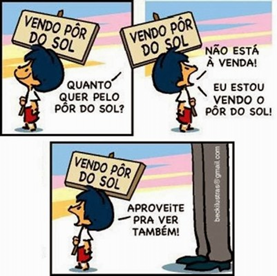
\includegraphics[width=2.88542in,height=2.875in]{./imgSAEB_7_POR/media/image4.png}

\href{https://tirasarmandinho.tumblr.com/}{\uline{https://tirasarmandinho.tumblr.com/}}
Acesso em 11 de Abr. de 2023
\end{quote}

\begin{enumerate}
\def\labelenumi{\arabic{enumi})}
\tightlist
\item
  Na tirinha acima pode-se perceber que o humor está presente. Qual a
  palavra está sendo usada para produzir este efeito?
\end{enumerate}

A palavra `vendo'

\begin{enumerate}
\def\labelenumi{\arabic{enumi})}
\setcounter{enumi}{1}
\tightlist
\item
  Por que o uso desta palavra produz efeito de humor?
\end{enumerate}

Porque a palavra vendo tem dois sentidos diferentes.

\begin{enumerate}
\def\labelenumi{\arabic{enumi})}
\setcounter{enumi}{2}
\tightlist
\item
  Quais as possíveis interpretações da palavra usada para produzir
  efeito de humor na tirinha?
\end{enumerate}

A palavra vendo pode significar o verbo ver, no particípio ou o verbo
vender no presente do indicativo, gerando sentidos diferentes, apesar da
grafia igual

\begin{enumerate}
\def\labelenumi{\arabic{enumi})}
\setcounter{enumi}{3}
\tightlist
\item
  Em qual sentido a palavra vendo está sendo usada pelo personagem
  Armandinho?
\end{enumerate}

No sentido do verbo ver

\begin{enumerate}
\def\labelenumi{\arabic{enumi})}
\setcounter{enumi}{4}
\tightlist
\item
  Em qual sentido está sendo compreendida a palavra vendo pelo adulto?
\end{enumerate}

No sentido de vender

\begin{enumerate}
\def\labelenumi{\arabic{enumi})}
\setcounter{enumi}{5}
\tightlist
\item
  Em qual quadrinho a questão das diferentes interpretações da palavra
  se esclarece?
\end{enumerate}

No último quadrinho

Analise a charge abaixo e responda:

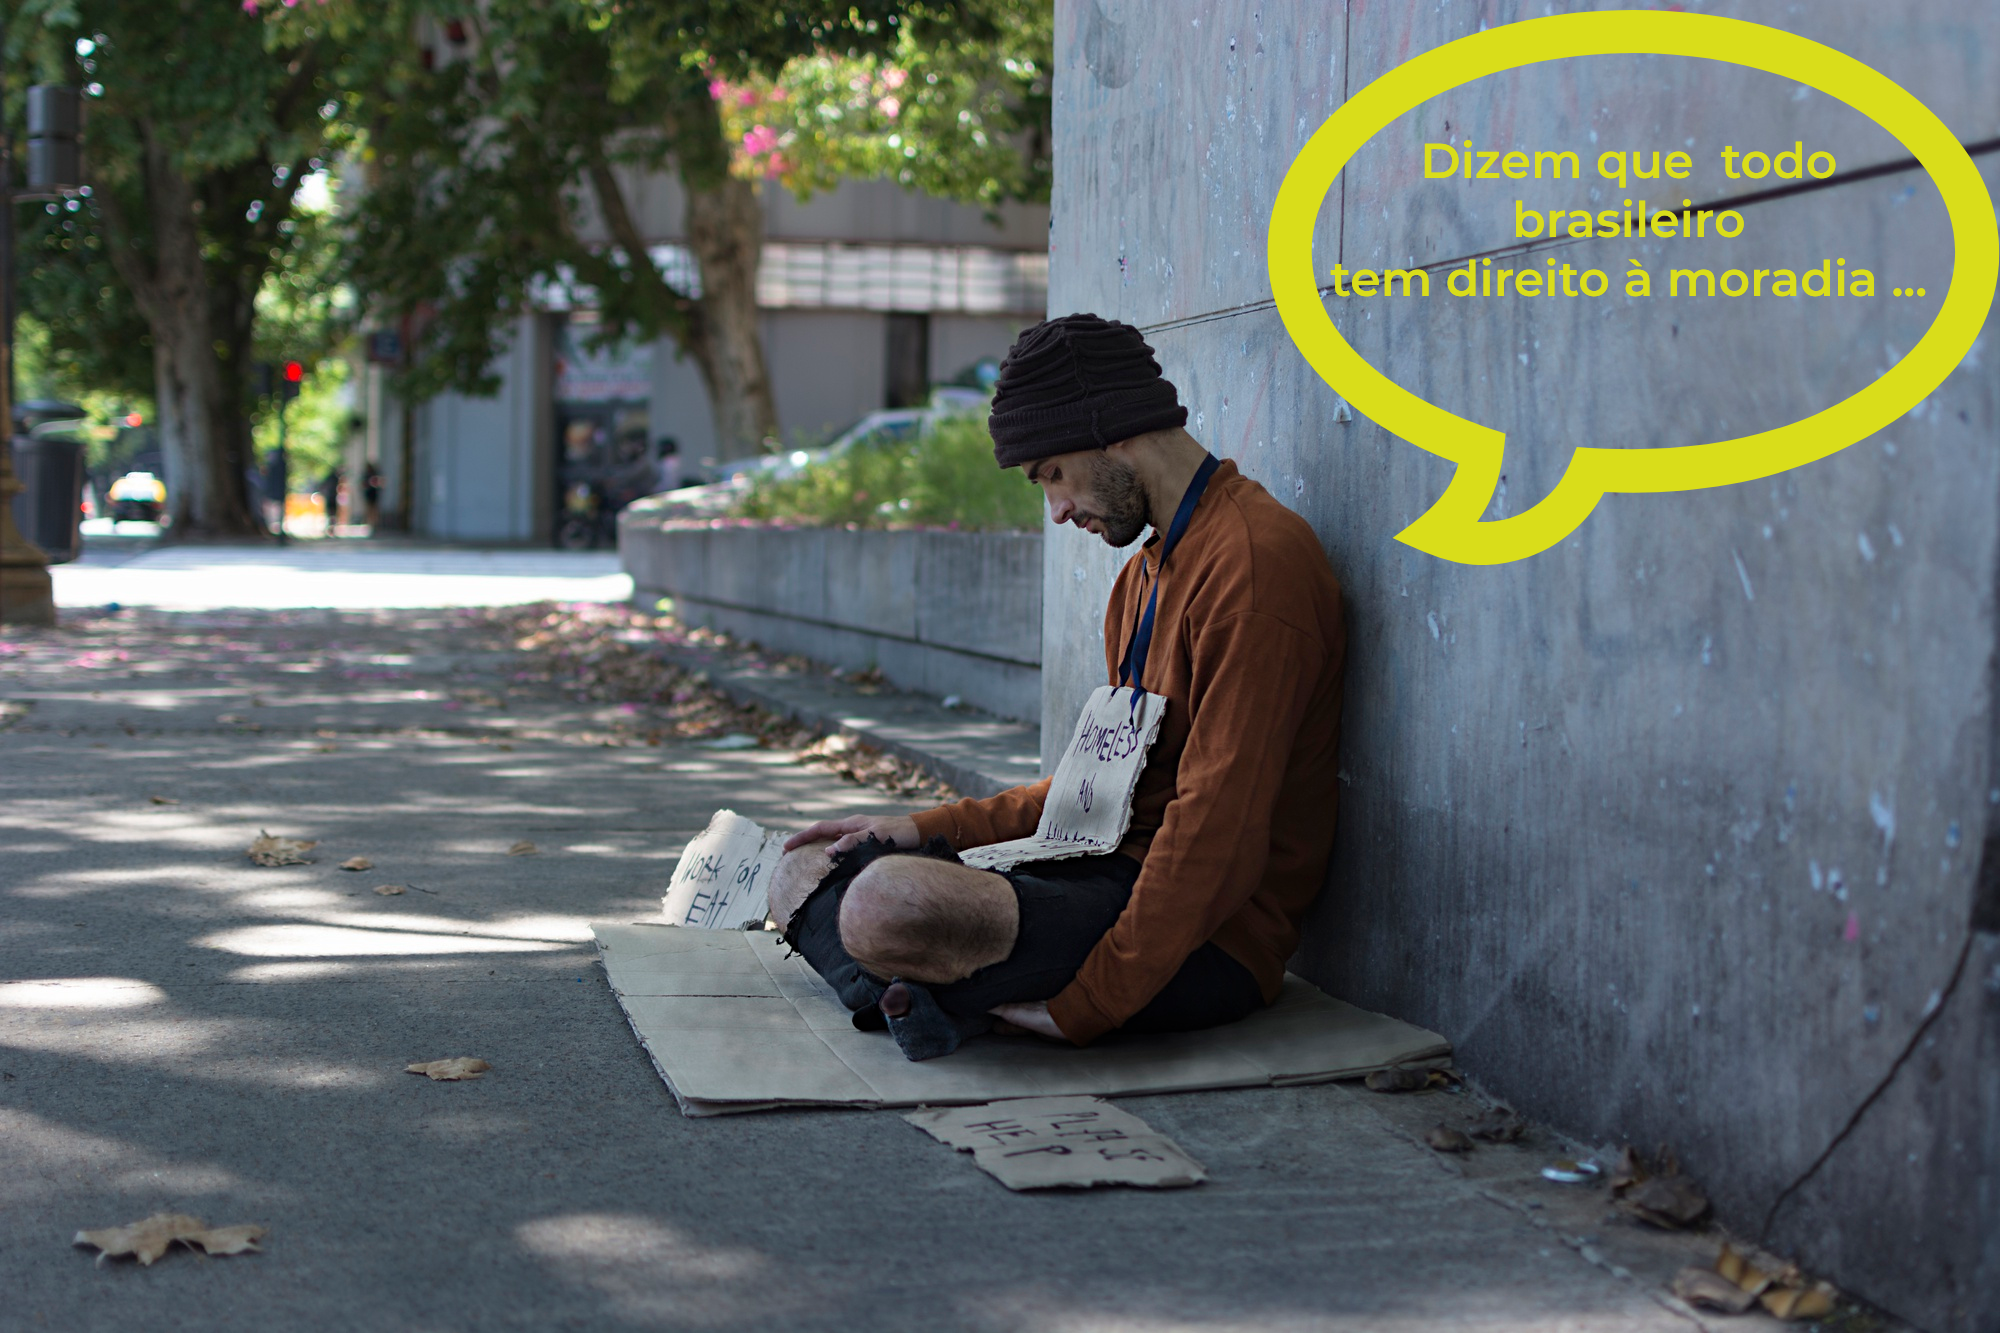
\includegraphics[width=5in,height=3.65625in]{./imgSAEB_7_POR/media/image5.png}

\href{http://www.arionaurocartuns.com.br/search/label/charges?updated-max=2022-12-15T14:30:00-08:00\&max-results=20\&start=40\&by-date=false}{\uline{http://www.arionaurocartuns.com.br/search/label/charges?updated-max=2022-12-15T14:30:00-08:00\&max-results=20\&start=40\&by-date=false}}
Acesso em 11 de abr de 2023

\begin{enumerate}
\def\labelenumi{\arabic{enumi})}
\setcounter{enumi}{6}
\tightlist
\item
  Segundo a imagem, o livro que o homem segura faz referência a um
  importante documento brasileiro. Que documento é esse?
\end{enumerate}

A constituição federal de 1988

\begin{enumerate}
\def\labelenumi{\arabic{enumi})}
\setcounter{enumi}{7}
\tightlist
\item
  Qual a função deste documento e o que ele pretende garantir?
\end{enumerate}

O documento trata das questões mais importantes para a manutenção da
democracia e pretende esclarecer os direitos e deveres de todos os
âmbitos da sociedade.

\begin{enumerate}
\def\labelenumi{\arabic{enumi})}
\setcounter{enumi}{8}
\tightlist
\item
  Qual o efeito de sentido explorado na charge?
\end{enumerate}

Ironia

\begin{enumerate}
\def\labelenumi{\arabic{enumi})}
\setcounter{enumi}{9}
\tightlist
\item
  De que forma a imagem se articula com o texto para produzir o efeito
  de sentido
\end{enumerate}

A charge apresenta ironia pois mostra o homem lendo a constituição
federal. Neste documento estão explicados os direitos de todos os
cidadãos, dentre eles a dignidade, o direito à moradia, acesso à saúde e
educação. Porém, se trata de um morador de rua que não teve tais
direitos garantidos.

\colorsec{Treino}

\num{1}

"Deus queira que o nosso alienista encontre muitos loucos. É o que lhe
desejo, com toda a minha alma. A ele e a todos que se derem ao estudo
das moléstias mentais, em benefício da humanidade."

Nesse trecho, qual o efeito de sentido utilizado pelo autor para mostrar
a falta de preocupação das pessoas da cidade com o tratamento dos
doentes mentais. Assinale a alternativa correta:

\begin{enumerate}
\def\labelenumi{\alph{enumi})}
\item
  ironia
\item
  duplo sentido
\item
  contradição
\item
  não há efeito de sentido
\end{enumerate}

\begin{enumerate}
\def\labelenumi{\alph{enumi})}
\item
  Correta. O desejo de que encontre `muitos loucos' apresenta ironia
  pois, o objetivo de quem trata de doenças mentais é que o número de
  pessoas que sofrem diminua e não aumente
\item
  Incorreta. Não há indicação de duplo sentido na frase
\item
  Incorreta. Não indicação de ambiguidade no trecho
\item
  Incorreta. Existe o uso da ironia como efeito de sentido
\end{enumerate}

Saeb: Inferir, em textos multissemiótico, efeitos de humor, ironia e/ou
crítica

Nível fácil

\num{2}

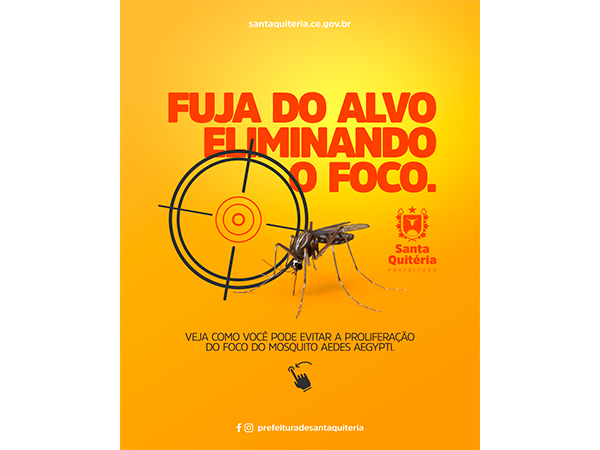
\includegraphics[width=5.90551in,height=4.43056in]{./imgSAEB_7_POR/media/image6.png}

\href{https://www.santaquiteria.ce.gov.br/informa.php?id=1018}{\uline{https://www.santaquiteria.ce.gov.br/informa.php?id=1018}}
. Acesso em 11 de abril de 2023.

Na imagem acima vemos uma campanha para evitar a proliferação do
mosquito da dengue. A escolha das palavras e imagens tem como objetivo
sensibilizar a população. Assinale a alternativa que contém as palavras
usadas para a produção de efeito de sentido na campanha:

\begin{enumerate}
\def\labelenumi{\alph{enumi})}
\item
  Proliferação e foco
\item
  Veja e evitar
\item
  Fuja e elimine
\item
  Alvo e foco
\end{enumerate}

Saeb: Inferir, em textos multissemiótico, efeitos de humor, ironia e/ou
crítica

Bncc:(EF69LP05) Inferir e justificar, em textos multissemióticos --
tirinhas, charges, memes, gifs etc. --, o efeito de humor, ironia e/ou
crítica pelo uso ambíguo de palavras, expressões ou imagens ambíguas, de
clichês, de recursos iconográficos, de pontuação etc.

\begin{enumerate}
\def\labelenumi{\arabic{enumi}.}
\tightlist
\item
  Incorreta. essas palavras não estão sendo usadas com sentido de
  ambiguidade
\end{enumerate}

b)Incorreta. essas palavras não estão sendo utilizadas para a produção
de efeitos de sentido

c)Incorreta. Não são estas as palavras que produzem efeitos de sentido
mais importantes no texto

\begin{enumerate}
\def\labelenumi{\arabic{enumi}.}
\tightlist
\item
  Correta. O uso das palavras foco e alvo produzem efeitos de sentido de
  ambiguidade e podem chamar a atenção da população para o problema e a
  forma de enfrentá-lo
\end{enumerate}

Nível médio

\num{3}

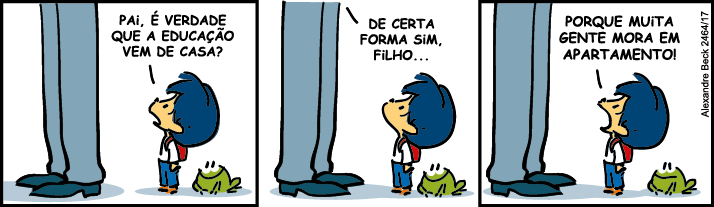
\includegraphics[width=5.90551in,height=1.70833in]{./imgSAEB_7_POR/media/image7.png}

\href{https://tirasarmandinho.tumblr.com/}{\uline{https://tirasarmandinho.tumblr.com/}}
Acesso em 12 de abr 2023.

Leia a tirinha acima e a assinale a alternativa que apresenta o efeito
de sentido produzido:

\begin{enumerate}
\def\labelenumi{\alph{enumi})}
\item
  a tirinha apresenta ironia sobre a educação com o uso ambíguo da
  palavra casa
\item
  a tirinha apresenta crítica à falta de moradia com o uso da palavra
  casa
\item
  a tirinha apresenta uma crítica às pessoas que moram em casas
\item
  a tirinha questiona o fato de pessoas morarem em apartamentos e não em
  casas
\end{enumerate}

Saeb: Inferir, em textos multissemiótico, efeitos de humor, ironia e/ou
crítica

Bncc:(EF69LP05) Inferir e justificar, em textos multissemióticos --
tirinhas, charges, memes, gifs etc. --, o efeito de humor, ironia e/ou
crítica pelo uso ambíguo de palavras, expressões ou imagens ambíguas, de
clichês, de recursos iconográficos, de pontuação etc.

\begin{enumerate}
\def\labelenumi{\arabic{enumi}.}
\tightlist
\item
  Correta. A palavra casa é utilizada em dois sentidos diferentes
\end{enumerate}

b)Incorreta. a tirinha não critica a falta de moradia e sim apresenta
uma ironia sobre a educação das pessoas

\begin{enumerate}
\def\labelenumi{\arabic{enumi}.}
\tightlist
\item
  Incorreta a tirinha não apresenta esse tipo de crítica
\end{enumerate}

d)Incorreta. a tirinha não faz alusão a esse fato

Nível difícil


\chapter{Parcialidade nos textos jornalísticos}
\markboth{Módulo 7}{}

\colorsec{Habilidades do SAEB}

\begin{itemize}

  \item Analisar marcas de parcialidade em textos jornalísticos.

  \item Avaliar diferentes graus de parcialidade em textos jornalísticos.

  \item Avaliar a fidedignidade de informações sobre um mesmo fato divulgado 
  em diferentes veículos e mídias.

\end{itemize}

\colorsec{Habilidades da BNCC}

\begin{itemize}

  \item EF07LP02, EF67LP03, EF67LP04.

\end{itemize}

\conteudo{A função ideal do jornalismo é informar de forma imparcial e objetiva
fatos e notícias para com isso oferecer informações e ferramentas para a
formação de opinião. No entanto, nem sempre é possível separar os fatos
das opiniões pois, todo texto, em alguma medida, é produzido a partir
das perspectivas pessoais do autor ou do veículo de comunicação que o
divulga. Por isso, é importante que os leitores aprendam a analisar
marcas de parcialidade em textos jornalísticos, a fim de avaliar o grau
de confiabilidade das informações que estão recebendo.

Uma das formas de identificar as marcas de parcialidade em textos
jornalísticos é perceber o conjunto de valores expressos pelo uso de
adjetivos, advérbios e na forma como são construídos os argumentos nos
textos de divulgação de notícias e acontecimentos. Também a escolha de
fontes e a seleção editorial dos assuntos e temas a serem tratados podem
indicar interesses e, portanto, certo grau de parcialidade. A escolha
dos pontos de vista expressos em uma notícia ou reportagem revela muito
sobre as intenções do autor ou do veículo que divulga o texto. Sendo
assim, comparar fontes e analisar de forma atenta os contextos em que as
informações são divulgadas em cada veículo de informação pode ser uma
forma eficaz de avaliar a confiabilidade e fidedignidade de determinada
notícia ou reportagem. Isso porque, a linha editorial e a relação dos
veículos de comunicação com empresas e grupos políticos ou econômicos
podem revelar possíveis interesses e pontos de vista. Portanto, aprender
a avaliar tais marcas de parcialidade e comparar diferentes formas de
divulgação de notícias em diversos veículos e texto é uma habilidade
importante para que o leitor possa formar uma opinião de forma reflexiva
e autônoma.}

\coment{Professor(a), faça um exercício de reflexão com os estudantes,
questionando como percebem os traços e interesses presentes em algumas
manchetes, e chamadas. Chame a atenção para veículos sensacionalistas,
para determinados temas e assuntos abordados e veiculados com a intenção
de gerar polêmicas, discussões ou busca de soluções. Converse com os
estudantes sobre os diversos tipos de textos jornalísticos e estimule-os
a refletir sobre como percebem as marcas de parcialidade. Instrua-os a
pesquisar e questionar os veículos de comunicação trazendo para a
discussão quais podem ser os interesses por trás dos recursos e
elementos multissemióticos presentes nas informações que consomem. Cite
a monetização de determinados conteúdos, explique como é importante
analisar quem são os financiadores e quais as propagandas e empresas
relacionadas aos veículos de informação que conhecem.}

\colorsec{Atividades}

\begin{quote}
Analise as duas notícias abaixo e responda as questões
\end{quote}

\begin{longtable}[]{@{}
  >{\raggedright\arraybackslash}p{(\columnwidth - 0\tabcolsep) * \real{0.9861}}@{}}
\toprule
\endhead
\textbf{Cinco desafios para a economia mundial em 2023}

Se 2022 foi um ano difícil para a economia global, 2023 promete ser
ainda pior, com uma recessão a caminho. Mas nem tudo será desgraça.

Espera-se que 2023 seja o terceiro ano com o pior crescimento econômico
global neste século, atrás de 2009, quando a crise financeira global
causou a Grande Recessão, e 2020, quando os lockdowns da covid-19
virtualmente paralisaram a economia global.

Analistas esperam que as principais economias do mundo, incluindo os
Estados Unidos e o Reino Unido, assim como a zona do euro, entrem em
recessão este ano, já que os bancos centrais continuam aumentando as
taxas de juros para moderar a demanda por bens de consumo e serviços, em
um esforço para conter a inflação. \\
\bottomrule
\end{longtable}

\begin{quote}
\href{https://www.dw.com/pt-br/cinco-desafios-para-a-economia-mundial-em-2023/a-64264182}{\uline{https://www.dw.com/pt-br/cinco-desafios-para-a-economia-mundial-em-2023/a-64264182}}
. Acesso em 11 de abri 2023
\end{quote}

\begin{longtable}[]{@{}
  >{\raggedright\arraybackslash}p{(\columnwidth - 0\tabcolsep) * \real{0.9861}}@{}}
\toprule
\endhead
\textbf{Por que a inflação mundial deve cair em 2023 (e por que a
notícia não é tão boa)}

Provavelmente o pior em termos de inflação já passou.

Pelo menos este é o consenso entre os economistas e as principais
organizações econômicas como o Fundo Monetário Internacional (FMI) ou o
Banco Mundial depois que a maioria dos países do mundo experimentou, em
2022, aumentos de preços não vistos em quatro décadas.

Não há dúvida de que a inflação continuará a pesar no bolso de milhões
de cidadãos em 2023, mas deve registrar uma queda lenta nos próximos 12
meses.

Quando esse período terminar, o FMI espera que a inflação mundial caia
para 4,7\%, pouco menos da metade do nível atual. \\
\bottomrule
\end{longtable}

\begin{quote}
\href{https://www.bbc.com/portuguese/internacional-64145595}{\uline{https://www.bbc.com/portuguese/internacional-64145595}}.
Acesso em 10 de abr de 2023
\end{quote}

\begin{enumerate}
\def\labelenumi{\arabic{enumi})}
\tightlist
\item
  Qual é o fato central de cada notícia?
\end{enumerate}

O fato central das duas notícias é a crise econômica

\begin{enumerate}
\def\labelenumi{\arabic{enumi})}
\setcounter{enumi}{1}
\tightlist
\item
  Quais são as semelhanças entre os fatos noticiados sobre o tema?
\end{enumerate}

As duas notícias tratam da recessão e da influência da queda da inflação
da crise econômica mundial

\begin{enumerate}
\def\labelenumi{\arabic{enumi})}
\setcounter{enumi}{2}
\tightlist
\item
  Quais são as diferenças entre os fatos noticiados sobre o tema?
\end{enumerate}

No primeiro exemplo tem-se uma previsão de crise pelo terceiro ano. Já
no segundo ano tem-se que, apesar da queda da inflação, haverá crise e
recessão

\begin{enumerate}
\def\labelenumi{\arabic{enumi})}
\setcounter{enumi}{3}
\tightlist
\item
  Em qual das duas notícias a crise mundial é tratada com mais otimismo.
  Copie do texto um trecho que justifique sua resposta
\end{enumerate}

O exemplo dois traz a mensagem de forma mais amena e otimista. Um
exemplo : ``Provavelmente o pior em termos de inflação já passou.''

\begin{enumerate}
\def\labelenumi{\arabic{enumi})}
\setcounter{enumi}{4}
\tightlist
\item
  Relacione os títulos abaixo com a linha fina
\end{enumerate}

\begin{enumerate}
\def\labelenumi{(\arabic{enumi})}
\item
  Estudiosos alertam para os riscos de doenças cardiovasculares e o
  sedentarismo
\item
  Casos de dengue preocupam secretarias de saúde
\item
  O perigo está em casa: Pediatras alertam sobre o uso excessivo de
  telas por crianças e adolescentes
\item
  Covid-19: Informar para proteger.
\end{enumerate}

\begin{quote}
( ) Análise de hábitos de pacientes com problemas cardiovasculares traz
novas informações sobre como prevenir doenças crônicas

( ) Associação brasileira de pediatria publica estudo sobre os impactos
dos jogos e redes sociais na vida de adolescentes

( ) Ministério da saúde lança cartilha para informar a população sobre
as formas de contágio da doença

( ) Alerta foi dado às secretarias de saúde de todo país, especialmente
nas regiões em que se inicia o período de chuvas

(1) Análise de hábitos de pacientes com problemas cardiovasculares traz
novas informações sobre como prevenir doenças crônicas

(3) Associação brasileira de pediatria publica estudo sobre os impactos
dos jogos e redes sociais na vida de adolescentes

(4) Ministério da saúde lança cartilha para informar a população sobre
as formas de contágio da doença

(2) Alerta foi dado às secretarias de saúde de todo país, especialmente
nas regiões em que se inicia o período de chuvas
\end{quote}

\begin{enumerate}
\def\labelenumi{\arabic{enumi})}
\setcounter{enumi}{5}
\tightlist
\item
  Sobre a parcialidade dos textos jornalísticos assinale V para as
  afirmações verdadeiras e F para as afirmações falsas
\end{enumerate}

\begin{quote}
( ) A imparcialidade no jornalismo é importante pois promove a formação
de opinião a partir dos fatos apresentados na reportagem.

( ) O princípio da imparcialidade no jornalismo significa que o
jornalista não deve apresentar os diferentes pontos de vista e deixar
que o público forme sua própria opinião.

( ) A imparcialidade no jornalismo pode levar a erros de interpretação e
compreensão dos fatos por parte do público, prejudicando a credibilidade
da reportagem do jornalista.

( ) A falta de apresentação de fontes e dados confiáveis pode ser uma
característica de parcialidade por parte do jornalista ou do veículo de
comunicação colocando em dúvida a qualidade das notícias veiculadas.

(V) A imparcialidade no jornalismo é importante pois promove a formação
de opinião a partir dos fatos apresentados na reportagem.

(F) O princípio da imparcialidade no jornalismo significa que o
jornalista não deve apresentar os diferentes pontos de vista e deixar
que o público forme sua própria opinião.

(V) A parcialidade no jornalismo pode levar a erros de interpretação e
compreensão dos fatos por parte do público, prejudicando a credibilidade
da reportagem do jornalista.

(V) A falta de apresentação de fontes e dados confiáveis pode ser uma
característica de parcialidade por parte do jornalista ou do veículo de
comunicação, colocando em dúvida a qualidade das notícias veiculadas.
\end{quote}

\begin{enumerate}
\def\labelenumi{\arabic{enumi})}
\setcounter{enumi}{6}
\tightlist
\item
  Leia os exemplos abaixo e sublinhe as marcas de parcialidade:
\end{enumerate}

\begin{quote}
``Polícia age com violência contra manifestantes pacíficos''

``Deputado faz discurso inflamado em defesa dos direitos dos
trabalhadores''

'' Falas preconceituosas de senadores exibem a impunidade da classe
política no Brasil''

``Polícia age com \uline{violência} contra manifestantes
\uline{pacíficos}''

``Deputado faz \uline{discurso inflamado} em defesa dos direitos dos
trabalhadores''

'' \uline{Falas preconceituosas} de senadores exibem a
\uline{impunidade} da classe política no Brasil''
\end{quote}

\begin{enumerate}
\def\labelenumi{\arabic{enumi})}
\setcounter{enumi}{7}
\tightlist
\item
  Quais aspectos devem ser levados em conta para questionar a
  parcialidade ou imparcialidade de uma notícia
\end{enumerate}

Os aspectos que devem ser levados em conta são a exposição de mais de um
ponto de vista sobre o mesmo tema, a citação de dados e pesquisas de
fontes confiáveis e o uso ou não de adjetivos que qualifiquem os fatos
apresentados. É importante também a checagem da veracidade dos dados
apresentados e o questionamento sobre os contextos em que ocorrem os
fatos e se há interesses políticos ou econômicos por parte do veículo de
comunicação que divulga a notícia

\begin{enumerate}
\def\labelenumi{\arabic{enumi})}
\setcounter{enumi}{8}
\tightlist
\item
  Analise as duas afirmações a seguir e responda qual das duas apresenta
  maior grau de parcialidade. Justifique sua resposta
\end{enumerate}

1.Policiamento nas cidades não geram mais segurança, é o que afirmam
especialistas

\begin{enumerate}
\def\labelenumi{\arabic{enumi}.}
\tightlist
\item
  Policiamento nas cidades é a principal medida de segurança anunciada
  pela prefeitura.
\end{enumerate}

A afirmação 1 apresenta maior grau de parcialidade pois defende uma
posição, mesmo que apoiada em afirmações de especialistas. No segundo
exemplo traz a notícia de maneira impessoal destacando o fato.

\begin{enumerate}
\def\labelenumi{\arabic{enumi})}
\setcounter{enumi}{9}
\tightlist
\item
  De que forma a apresentação de imagens, gráficos e tabelas auxiliam na
  formação de opinião de leitores?
\end{enumerate}

Imagens e gráficos podem contribuir para embasar as informações e trazem
mais confiabilidade à notícia pois podem ser interpretados, questionados
e verificados.

\colorsec{Treino}

\num{1}

Sabendo da importância de aprender a analisar traços de parcialidade em
textos jornalísticos, assinale a alternativa que contém uma forma de
detectar parcialidade em um texto jornalístico?

\begin{enumerate}
\def\labelenumi{\alph{enumi})}
\item
  A presença de entrevistas com especialistas no assunto abordado.
\item
  A apresentação de diferentes pontos de vista sobre o mesmo assunto.
\item
  A utilização de adjetivos valorativos para descrever pessoas ou
  eventos.
\item
  A verificação da presença de fatos e fontes citadas
\end{enumerate}

Saeb: Analisar marcas de parcialidade em textos jornalísticos.

a)Incorreta. Este é um traço de imparcialidade

\begin{enumerate}
\def\labelenumi{\arabic{enumi}.}
\item
  Incorreta. A apresentação de diferentes pontos de vista é uma forma de
  garantir imparcialidade
\item
  Correta. A presença de adjetivos caracteriza a opinião do autor e é
  uma marca de parcialidade
\item
  Incorreta. A presença de fontes e fatos garante certa imparcialidade
\end{enumerate}

Nível fácil

\num{2}

Leia o trecho abaixo e o gráfico que segue:

``Não estamos no caminho certo para atingir as metas de mudança
climática. Se somarmos todas as promessas para reduzir emissões de gases
que provocam efeito estufa pelos países que assinaram o Acordo de Paris,
o mundo ainda esquentaria em mais de 3°C até o fim deste século''

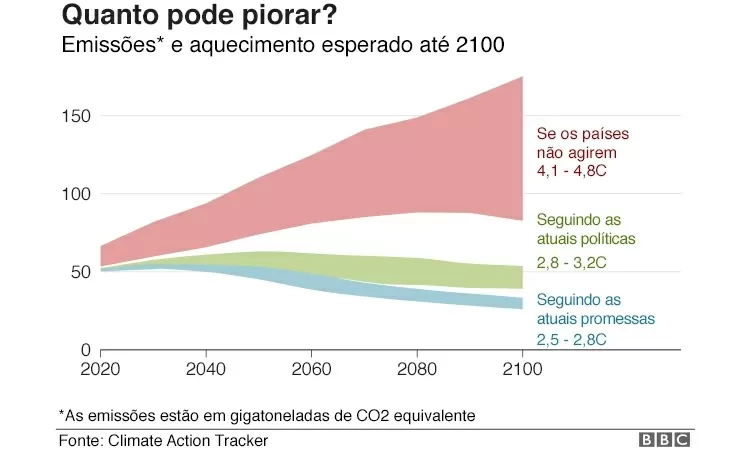
\includegraphics[width=5.90551in,height=3.56944in]{./imgSAEB_7_POR/media/image8.png}

\href{https://www.bbc.com/portuguese/geral-46424720}{\uline{https://www.bbc.com/portuguese/geral-46424720}}
Acesso em 13 de Abr de 2023

Assinale a alternativa que contém o principal recurso de suporte para a
confiabilidade da notícia:

\begin{enumerate}
\def\labelenumi{\alph{enumi})}
\item
  a opinião do jornalista
\item
  a citação do Acordo de Paris
\item
  o uso de gráficos de pesquisas sobre mudanças climáticas
\item
  o uso de expressões que pretendem sensibilizar o leitor
\end{enumerate}

Saeb:Avaliar diferentes graus de parcialidade em textos jornalísticos.

\begin{enumerate}
\def\labelenumi{\arabic{enumi}.}
\item
  Incorreta. A opinião do jornalista não é um recurso de imparcialidade
\item
  Incorreta. Embora o Acordo de Paris seja um documento importante, ele
  é citado como para se referir às metas de ambientais para reverter a
  situação climática
\item
  Correta. O uso de gráficos e recursos do tipo trazem maior clareza
  possibilitando ao leitor formar suas próprias opiniões
\item
  Incorreta. O uso de expressões que pretendem sensibilizar o leitor são
  recursos de persuasão importantes, porém não conferem imparcialidade
  ao texto
\end{enumerate}

Nível médio

\num{3}

``Após três anos sem reajuste, tarifa de ônibus é corrigida abaixo da
inflação do período''

A partir de 1° de janeiro de 2023, o transporte coletivo urbano de
Joinville passará a operar com os valores de R\$5,25 para a tarifa
antecipada e R\$5,50 para a tarifa embarcada (modalidade utilizada por
apenas 5\% dos passageiros). O reajuste representa aproximadamente
metade do percentual de inflação dos últimos três anos, período no qual
a tarifa não foi corrigida.

https://www.joinville.sc.gov.br/noticias/apos-tres-anos-sem-reajuste-tarifa-de-onibus-e-corrigida-abaixo-da-inflacao-do-periodo/
Acesso em 11 de abri 2023

A matéria apresenta grau de parcialidade pois:

\begin{enumerate}
\def\labelenumi{\alph{enumi})}
\item
  Apresenta a justificativa para o aumento e argumenta sobre ainda estar
  abaixo da inflação
\item
  Apresenta informações precisas sobre a data do ocorrido
\item
  Apresenta informações sobre os valores da passagem
\item
  Apresenta dados sobre os usuários do transporte público na cidade
\end{enumerate}

Saeb:Analisar marcas de parcialidade em textos jornalísticos.

\textbf{(EF67LP04)} Distinguir, em segmentos descontínuos de textos,
fato da opinião enunciada em relação a esse mesmo fato.

a)Correta. Já no título a notícia traz argumentos que levam a crer na
necessidade de reajuste

\begin{enumerate}
\def\labelenumi{\arabic{enumi}.}
\item
  Incorreta. As informações sobre data e local são partes importantes da
  transmissão da notícia de forma imparcial
\item
  Incorreta. Estas informações não representam a opinião do veículo e
  poderiam ser considerados recursos para atribuir veracidade à notícia
\item
  Incorreta. Estes dados não representam a opinião do veículo e poderiam
  ser considerados recursos para corroborar a tese afirmada no título
\end{enumerate}

Nível difícil

\chapter{Recursos de modalização e argumentação}
\markboth{Módulo 8}{}

\colorsec{Habilidades do SAEB}

\begin{itemize}

  \item Identificar os recursos de modalização em textos diversos.

  \item Analisar os efeitos de sentido dos tempos, modos e/ou vozes 
verbais com base no gênero textual e na intenção comunicativa.

  \item Analisar os efeitos de sentido produzidos pelo uso de modalizadores em textos diversos.

\end{itemize}

\colorsec{Habilidades da BNCC}

\begin{itemize}

  \item EF69LP04, EF69LP28, EF07LP14.

\end{itemize}

\conteudo{A capacidade de identificar e compreender os recursos de modalização
presentes em diferentes tipos de texto é fundamental para uma
comunicação eficiente e coerente. A modalização envolve o uso de
recursos linguísticos para expressar atitudes e opiniões do emissor em
relação ao conteúdo abordado, sendo que esses recursos podem estar
presentes nas formas de uso de verbos, adjetivos, advérbios, modos e
vozes.

A análise dos efeitos de sentido produzidos pelos recursos de
modalização em diferentes gêneros textuais e intenções comunicativas é
fundamental para identificar as influências destes recursos na percepção
e compreensão do conteúdo pelo receptor.

Os recursos de modalização permitem que o emissor expresse suas
opiniões, transmita suas expectativas, faça indicações, influenciando
assim na percepção e na ação dos leitores. Dentre os principais recursos
de modalização, encontram-se os tempos verbais, os modos verbais, as
vozes verbais e os modalizadores, que podem reformar graus de
probabilidade, certeza, necessidade e urgência.

Portanto, compreender e utilizar os recursos de modalização de forma
adequada é essencial para produzir textos claros, coerentes e
persuasivos, adaptando a linguagem ao tipo de público alvo e ao contexto
em que são emitidos. Além disso, a análise crítica desses recursos
permite que o leitor compreenda as intenções do emissor e as influências
que podem estar presentes no conteúdo do texto.}

\coment{Professor(a), estimule os estudantes a lembrarem do uso destes recursos
em exemplos conhecidos e práticos tais como campanhas de conscientização
ou publicitárias. Retome os recursos de modalização presentes em
diversos gêneros textuais já estudados demonstrando as diferenças de
interpretação e sentido possíveis para os usos de tempos e modos
verbais, tais como infinitivo e imperativo, das vozes do texto, dos
discursos diretos e indiretos e do uso de advérbios que qualificam as
ações com advérbios que indicam urgência, condições, sugestões,
obrigatoriedade, etc}

\colorsec{Atividades}


\includegraphics[width=2.85536in,height=2.85536in]{./imgSAEB_7_POR/media/image9.png}

\href{https://itajuba.mg.gov.br/secretariaspmi/semdes/nao_desvie_o_olhar/}{\uline{https://itajuba.mg.gov.br/secretariaspmi/semdes/nao\_desvie\_o\_olhar/}}.
Acesso em 18 de abr de 2023

\begin{enumerate}
\def\labelenumi{\arabic{enumi})}
\tightlist
\item
  Retire da imagem acima,os elementos modalizadores que produzem o
  sentido de instrução.
\end{enumerate}

O uso dos verbos no imperativo

\begin{enumerate}
\def\labelenumi{\arabic{enumi})}
\setcounter{enumi}{1}
\tightlist
\item
  De que forma o uso desses recursos sensibiliza o leitor
\end{enumerate}

A escolha dos verbos apelam para a responsabilidade individual de cada
um enquanto cidadão

\begin{enumerate}
\def\labelenumi{\arabic{enumi})}
\setcounter{enumi}{2}
\tightlist
\item
  Observe as informações contidas no cartaz e responda qual a ação
  recomendada ao tomar conhecimento de casos de violência contra
  crianças e adolescentes?
\end{enumerate}

Ligar para o telefone indicado

\begin{enumerate}
\def\labelenumi{\arabic{enumi})}
\setcounter{enumi}{3}
\tightlist
\item
  Relacione as colunas de expressões com seus respectivos efeitos de
  sentido:
\end{enumerate}

\begin{quote}
( I )Obrigação

(II) Apreciação

(III) Possibilidade

(IV) Certeza

( ) felizmente

( ) é dever de todos

( ) é impossível

( ) provavelmente

(II) felizmente

(I) é dever de todos

(IV) é impossível

(III) provavelmente
\end{quote}

Leia a afirmação abaixo e responda:

\begin{quote}
\textbf{Certamente}, com a implementação dos projetos de mobilidade
urbana, as pessoas passarão a ter mais qualidade de vida e mais
liberdade para explorar e ocupar a cidade.
\end{quote}

\begin{enumerate}
\def\labelenumi{\arabic{enumi})}
\setcounter{enumi}{4}
\tightlist
\item
  Qual sentido a palavra destacada pretende expressar?
\end{enumerate}

Pretende expressar certeza sobre as consequências da melhoria da
mobilidade urbana.

\begin{quote}
Observe a campanha a seguir e responda:


\includegraphics[width=5.90551in,height=1.47222in]{./imgSAEB_7_POR/media/image10.png}

\href{http://www.artesp.sp.gov.br/Style\%20Library/extranet/campanha-interna.aspx?id=1}{\uline{http://www.artesp.sp.gov.br/Style\%20Library/extranet/campanha-interna.aspx?id=1}}.
Acesso em 18 de abr de 2023.
\end{quote}

\begin{enumerate}
\def\labelenumi{\arabic{enumi})}
\setcounter{enumi}{5}
\tightlist
\item
  Observe o uso da conjunção ``se'' na frase, 'Neste carnaval se beber,
  não dirija''. Qual a ideia transmitida por este recurso?
\end{enumerate}

\begin{quote}
A ideia da conjunção é propor um impeditivo ou condição. Neste caso,
para dirigir é necessário não ingerir álcool
\end{quote}

\begin{enumerate}
\def\labelenumi{\arabic{enumi})}
\setcounter{enumi}{6}
\tightlist
\item
  Ainda sobre a campanha acima, assinale verdadeiro ou falso para as
  afirmações a seguir
\end{enumerate}

\begin{quote}
( ) a campanha sugere que não se pode dirigir após beber

( ) a campanha sugere que as pessoas não devem beber durante o carnaval

( ) a campanha orienta os foliões a não dirigir no carnaval

( ) a campanha pretende alertar sobre a violência no trânsito

( ) a campanha faz uso da conjunção condicional para sensibilizar o
público

(V) a campanha sugere que não se pode dirigir após beber

(F) a campanha sugere que as pessoas não devem beber durante o carnaval

(F) a campanha orienta os foliões a não dirigir no carnaval

(F ) a campanha pretende alertar sobre a violência no trânsito

(V) a campanha faz uso da conjunção condicional para sensibilizar o
público
\end{quote}

\begin{enumerate}
\def\labelenumi{\arabic{enumi})}
\setcounter{enumi}{7}
\tightlist
\item
  Leia os enunciados e enumere as proposições.
\end{enumerate}

\begin{enumerate}
\def\labelenumi{(\arabic{enumi})}
\item
  É necessária a presença de um acompanhante.
\item
  É proibida a entrada de acompanhante.
\item
  É permitida a entrada de um acompanhante.
\end{enumerate}

\begin{quote}
( ) Expressa proibição

( ) Expressa obrigatoriedade
\end{quote}

( ) Expressa permissão

\begin{quote}
(2) Expressa proibição

(1) Expressa obrigatoriedade
\end{quote}

(3) Expressa permissão

Leia tirinha abaixo:


\includegraphics[width=5.90551in,height=1.72222in]{./imgSAEB_7_POR/media/image11.png}

\href{https://tirasarmandinho.tumblr.com/}{\uline{https://tirasarmandinho.tumblr.com/}}
Acesso em 19 de Abr de 2023

\begin{enumerate}
\def\labelenumi{\arabic{enumi}.}
\tightlist
\item
  Qual é a confusão comunicativa presente na tirinha?
\end{enumerate}

A confusão se dá pois os personagens entendem o verbo falar em sentidos
diferentes

10) Qual o sentido do verbo falar no segundo quadrinho? Escreva um
sinônimo

O verbo falar no segundo quadrinho se refere a opinião, e poderia ser
substituído por dizer ou pensar. Pensaria, diria.

\colorsec{Treino}

\num{1}

Antes da pandemia causada pelo novo coronavírus, era quase impensável
ver grande parte da população usando máscaras de proteção na rua.
Contudo a situação mudou, principalmente após o governo do estado tornar
seu uso obrigatório. Mesmo assim, ainda há dúvidas de parte da população
quanto à necessidade e ao benefício do seu uso.

\href{https://coronavirus.saude.mg.gov.br/blog/101-mascaras-e-covid-19}{\uline{https://coronavirus.saude.mg.gov.br/blog/101-mascaras-e-covid-19}}.
Acesso em 19 de Abr. de 2023.

A expressão `mesmo assim' se refere:

\begin{enumerate}
\def\labelenumi{\alph{enumi})}
\item
  à determinação da obrigatoriedade do uso de máscaras pelo governo do
  estado
\item
  à mudança da situação quanto a pandemia de coronavírus
\item
  ao início da pandemia de coronavírus ter sido uma surpresa para toda a
  população
\item
  ao fato de ser impensável ver grande parte da população utilizando
  máscaras de proteção
\end{enumerate}

Saeb: Analisar os efeitos de sentido produzidos pelo uso de
modalizadores em

textos diversos.

Bncc:\textbf{(EF07LP14)}Identificar, em textos, os efeitos de sentido do
uso de estratégias de modalização e argumentatividade.

\begin{enumerate}
\def\labelenumi{\arabic{enumi}.}
\item
  Correta. A expressão faz alusão à frase anterior
\item
  Incorreta. O texto não indica mudanças na situação da pandemia
\end{enumerate}

c)Incorreta. O trecho em destaque não faz alusão a este posicionamento
do autor

d)Incorreta. O trecho em destaque não se refere a esta afirmação

Nível difícil

\num{2}
Observe a tirinha abaixo:

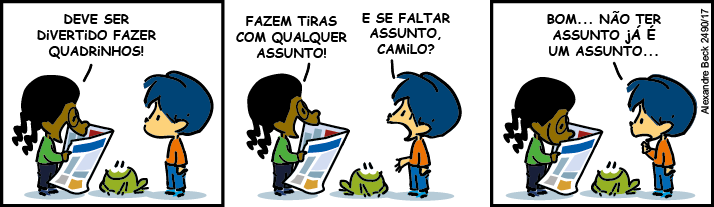
\includegraphics[width=5.90551in,height=1.70833in]{./imgSAEB_7_POR/media/image12.png}

\href{https://tirasarmandinho.tumblr.com/}{\uline{https://tirasarmandinho.tumblr.com/}}.
Acesso em 20 de Abr de 2023

O verbo deve no primeiro quadrinho expressa:

\begin{enumerate}
\def\labelenumi{\alph{enumi})}
\item
  Obrigação
\item
  Conselho
\item
  Causa
\item
  Possibilidade
\end{enumerate}

Saeb:Analisar os efeitos de sentido dos tempos, modos e/ou vozes verbais
com

base no gênero textual e na intenção comunicativa.

a)Incorreta. O verbo dever neste caso não indica obrigatoriedade

b)Incorreta. O verbo deve neste caso não indica conselho

c)Incorreta. Não há relação de causa na fala do primeiro quadrinho

d)Correta. Esta variação do uso do verbo dever indica uma possibilidade,
uma suposição

Nível fácil

\num{3}

Analise o cartaz abaixo:


\includegraphics[width=5.90551in,height=4.29167in]{./imgSAEB_7_POR/media/image13.png}

\href{https://www.gov.br/dnocs/pt-br/assuntos/noticias/consumo-consciente-da-agua-e-base-para-um-futuro-sustentavel}{\uline{https://www.gov.br/dnocs/pt-br/assuntos/noticias/consumo-consciente-da-agua-e-base-para-um-futuro-sustentavel}}.
Acesso em 20 de Abr de 2023

O uso dos verbos no gerúndio em campanhas de conscientização é comum
pois expressa:

\begin{enumerate}
\def\labelenumi{\alph{enumi})}
\item
  O desenvolvimento de uma ação duradoura.
\item
  Uma ordem a ser acatada
\item
  Um sugestão a ser considerada
\item
  Uma ação que já aconteceu
\end{enumerate}

Saeb: Analisar os efeitos de sentido dos tempos, modos e/ou vozes
verbais com

base no gênero textual e na intenção comunicativa.

Bncc: \textbf{(EF69LP04)} Identificar e analisar os efeitos de sentido
que fortalecem a persuasão nos textos publicitários, relacionando as
estratégias de persuasão e apelo ao consumo com os recursos
linguístico-discursivos utilizados, como imagens, tempo verbal, jogos de
palavras, figuras de linguagem etc., com vistas a fomentar práticas de
consumo conscientes.

\begin{enumerate}
\def\labelenumi{\arabic{enumi}.}
\item
  Correta. O verbo no gerúndio dá ideia de continuidade para a ação.
\item
  Incorreta. A expressão de ordem geralmente utiliza o verbo no infinito
  ou imperativo
\item
  Incorreta. Para sugestões,normalmente são utilizados verbos no
  infinitivo ou imperativo
\item
  Incorreta. O verbo no gerúndio não se refere a uma ação ocorrida no
  passado, mas que ocorre no presente e pode continuar ocorrendo
\end{enumerate}

Nível difícil


\chapter{Figuras de linguagem como estratégia argumentativa}
\markboth{Módulo 9}{}

\colorsec{Habilidades do SAEB}

\begin{itemize}
  
  \item Analisar o uso de figuras de linguagem como estratégia argumentativa.

  \item Avaliar a eficácia das estratégias argumentativas em textos de diferentes gêneros.

\end{itemize}

\colorsec{Habilidades da BNCC}

\begin{itemize}

  \item EF69LP17, EF67LP38.

\end{itemize}

\conteudo{A linguagem tem como principal objetivo a comunicação, portanto, é
impossível distinguir a linguagem da interação que ela provoca. Quanto
maior o domínio das ferramentas de linguagem por parte do autor, maior o
nível de interação e conexão será atingido com o leitor. Do outro lado,
quanto maior a capacidade de reconhecimentos das ferramentas e recursos
de expressividade forem conhecidas pelo leitor, melhor será sua
experiência. Existem diversas maneiras de promover maior expressividade
das palavras e com isso, facilitar e potencializar a interação por meio
da comunicação. Dentre esses recursos estão as chamadas figuras de
linguagem. São expressões e formas de interação possíveis à linguagem
que podem trazer maior riqueza de detalhes, maior clareza ou maior
objetividade ao texto, seja ele escrito ou transmitido oralmente.

Cada figura de linguagem tem suas características próprias e pode ser
utilizada de diversas maneiras, de acordo com o objetivo do falante ou
do escritor, com a situação comunicativa e com o interlocutor. As
figuras de linguagem podem fazer alusão ao sentido figurado das palavras
e expressões, tratar com exagero para exacerbar características e
impressões ou contrapor palavras com sentidos antagônicos demonstrando
valores de forma implícita. Por essas características, as figuras de
linguagem são recursos comunicativos de grande utilidade especialmente
para escrita de textos do campo artístico literário como letras de
músicas e poemas. Se apresentam ainda como um recurso de persuasão e
comunicação importante também para os textos do campo jornalístico
midiático.

Sendo assim, a metáfora é uma figura de linguagem utilizada para
estabelecer uma relação de semelhança e comparação entre dois termos
distintos. Um exemplo do uso da metáfora é a expressão "sua vida era um
mar de rosas". Nesse caso, a expressão "mar de rosas" não tem o sentido
literal, mas sim o sentido figurado, pois se refere a algo agradável e
prazeroso e não ao mar em sentido literal.

A metonímia, por sua vez, é a figura de linguagem utilizada quando se
lança mão um termo para se referir a outro, com o qual ele mantém uma
relação de proximidade, continuidade e pertencimento. Ou seja, dizer que
"a cidade se beneficiou com as obras de infraestrutura" é utilizar a
figura de linguagem metonímia, pois, utiliza o termo ' a cidade' para se
referir à população da cidade. A metonímia tem o efeito de tornar a
linguagem mais concisa e precisa, evitando a repetição de termos e
textos muito extensos. É uma forma de dinamizar a comunicação e
potencializar a capacidade comunicativa.

Já a personificação é a figura de linguagem utilizada sempre que se
atribui a animais e objetos, características humanas. A personificação
tem o efeito de tornar a linguagem mais expressiva e poética, pois
humaniza seres e fenômenos produzindo alto grau de identificação do
leitor com a experiência, sensação ou impressão que se pretende
comunicar.

Por fim, a hipérbole é a figura de linguagem que aumenta ou exagera
determinada característica como forma de expressão, pode representar um
exagero para transmitir uma ideia.

\coment{Professor(a) peça aos estudantes que tragam suas impressões, faça um
levantamento dos conhecimentos prévios que já têm. Deixe que tragam
exemplos e forneça mais informações sobre os conceitos, chamando a
atenção para as possibilidades expressivas das figuras de linguagem.
Mostre como o uso das figuras de linguagem podem ampliar os efeitos de
sentido, seja nos textos literários, nos textos jornalísticos, para
efeitos de ironia, humor, etc.}

\colorsec{Atividades}

Que, havendo tanto já que as partes vendo

Onde o dia é comprido e onde breve,

Inclinam seu propósito e perfia

\textbf{A ver os berços onde nasce o dia}.'

Os Lusíadas I-27-8
\href{http://www.dominiopublico.gov.br/download/texto/bv000162.pdf}{\uline{http://www.dominiopublico.gov.br/download/texto/bv000162.pdf}}.
Acesso em 19 de abr de 2023

Analise o trecho destacado e responda:

\begin{enumerate}
\def\labelenumi{\arabic{enumi})}
\tightlist
\item
  Qual a figura de linguagem presente no verso em destaque?
\end{enumerate}

A figura de linguagem presente no verso é a personificação pois atribui
características humanas ao fenômeno natural do nascimento do sol.

\begin{enumerate}
\def\labelenumi{\arabic{enumi})}
\setcounter{enumi}{1}
\tightlist
\item
  Assinale nas opções abaixo as características da metáfora:
\end{enumerate}

( ) utilizada em textos poéticos

( ) faz comparação entre termos diferentes

( ) Apresenta o termo de comparação

( ) faz uma comparação sem utilizar o termo de comparação

(X) utilizada em textos poéticos

(X) faz comparação entre termos diferentes

( ) Apresenta o termo de comparação

(X) faz uma comparação sem utilizar o termo de comparação

O BURRO E O LEÃO Vinha o burro pelo caminho, na sua ignorância de
sempre. Numa curva, deparou com o leão. --- Saia já da minha frente ---
disse ele, com a presunção dos tolos. O leão olhou bem para o burro e
pensou: "Seria fácil demais dar uma lição a esse infeliz. Não vou sujar
meus dentes e minhas garras com ele." E prosseguiu, muito calmo, sem se
importar com o burro.

Acima, vemos o exemplo de uma fábula. As fábulas, em geral, apresentam
elementos da natureza e animais como personagens principais. Sabendo
disso, retire do texto exemplos de personificação:

O leão olhou bem para o burro e pensou. Dentre outros

\begin{enumerate}
\def\labelenumi{\arabic{enumi})}
\setcounter{enumi}{2}
\item
  Ao dizer a seguinte frase: Você tem um coração de pedra! Faz-se uso de
  qual figura de linguagem?
\item
  A afirmação `Estou morrendo de medo' sugere o uso de qual figura de
  linguagem?
\item
  As estrelas são os olhos dos deuses, representa qual figura de
  linguagem?
\item
  Associe as frases com a figura de linguagem correspondente:
\item
  Sobre a hiperbole, assinale V para as afirmações verdadeiras e F para
  as falsas:
\end{enumerate}

\begin{quote}
( ) Faz uma comparação entre palavras distintas

( ) pretende exagerar o sentido de uma palavra

( ) expressa ênfase em uma sensação

( ) atribui características humanas a objetos

(F) Faz uma comparação entre palavras distintas

(V) pretende exagerar o sentido de uma palavra

(V) expressa ênfase em uma sensação

( F) atribui características humanas a objetos

Na cordilheira que fica em cima do vale de Yyucay, em Cusco,

pode-se ouvir todos os sons. O vento sopra com sua bocarra;

a manhã, obrigada a se levantar sempre antes dos outros,

boceja morta de sono; os pássaros, seus eternos namorados,

acordam cantando ao ouvi-la se espreguiçar.

http://www.dominiopublico.gov.br/download/texto/me001614.pdf
\end{quote}

\begin{enumerate}
\def\labelenumi{\arabic{enumi})}
\setcounter{enumi}{7}
\tightlist
\item
  Quais as figuras de linguagem presentes no trecho acima:
\end{enumerate}

Hipérbole, personificação

\begin{enumerate}
\def\labelenumi{\arabic{enumi})}
\setcounter{enumi}{8}
\tightlist
\item
  Copie do texto um exemplo de hipérbole:
\end{enumerate}

boceja morta de sono

\begin{enumerate}
\def\labelenumi{\arabic{enumi})}
\setcounter{enumi}{9}
\tightlist
\item
  Copie do texto um exemplo de personificação
\end{enumerate}

O vento sopra com sua bocarra, os pássaros, seus eternos namorados,

acordam cantando ao ouvi-la se espreguiçar.

\colorsec{Treino}

\num{1}

``Brasil reforça postura de neutralidade e ganha espaço na geopolítica
mundial''

O trecho acima apresenta a figura de linguagem metonímia pois:

\begin{enumerate}
\def\labelenumi{\alph{enumi})}
\item
  Personifica o país
\item
  compara o Brasil com outros países
\item
  Exagera ao qualificar o Brasil como um país neutro
\item
  Usa o termo Brasil para se referir ao governo do país
\end{enumerate}

Saeb:Avaliar a eficácia das estratégias argumentativas em textos de
diferentes

gêneros.

a)Incorreta. A personificação não é característica da metonímia

b)Incorreta. O texto não faz comparação com outros países

c)Incorreta. O texto não faz alusão isso nem utiliza hipérbole

d)Correta. Nesta alternativa temos a definição de metonímia

Nível Médio

\num{2}

Ao voltar para casa, \textbf{não se cansava de elogiar} a

desconhecida do baile. Nos dias que se seguiram, procurou-a

por toda a fazenda e pelos povoados vizinhos, mas não

conseguiu encontrá-la. E ficou mais triste ainda.

O trecho destacado apresenta a figura de linguagem:

\begin{enumerate}
\def\labelenumi{\alph{enumi})}
\item
  metáfora
\item
  hipérbole
\item
  metonímia
\item
  personificação
\end{enumerate}

Saeb: Avaliar a eficácia das estratégias argumentativas em textos de
diferentes

gêneros.

\begin{enumerate}
\def\labelenumi{\arabic{enumi}.}
\tightlist
\item
  Incorreta. O trecho não faz comparação
\end{enumerate}

b)Correta. O trecho exagera o termo para expressar o quanto o rapaz
falava da moça

\begin{enumerate}
\def\labelenumi{\arabic{enumi}.}
\item
  Incorreta. O trecho não utiliza um termo para significar outro termo
  referente
\item
  Incorreta. O trecho não atribui características humanas a objetos
  inanimados ou fenômenos naturais.
\end{enumerate}

Nível Difícil

\num{3}

Leia a tirinha abaixo:

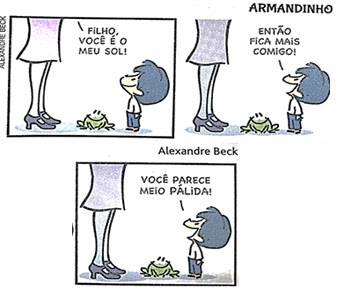
\includegraphics[width=3.51042in,height=3.02083in]{./imgSAEB_7_POR/media/image14.png}

\href{https://tirasarmandinho.tumblr.com/}{\uline{https://tirasarmandinho.tumblr.com/}}.
Acesso em 20 de Abr de 2023.

A mãe de Armandinho expressa seu amor pelo filho fazendo uso de:

\begin{enumerate}
\def\labelenumi{\alph{enumi})}
\item
  Hipérbole
\item
  Metáfora
\item
  Personificação
\item
  Metonímia
\end{enumerate}

Saeb: Analisar o uso de figuras de linguagem como estratégia
argumentativa.

a)Incorreta. Não há exagero ou ênfase na tirinha

b)Correta. A mãe faz uso da metáfora pois utiliza uma comparação

\begin{enumerate}
\def\labelenumi{\arabic{enumi}.}
\item
  Incorreta. Não há atribuição de características humanas ao sol e sim
  uma comparação
\item
  Incorreta. A tirinha não apresenta exemplo de metonímia
\end{enumerate}

Nível fácil


\chapter{Tecendo com as palavras: recursos de coesão e progressão textual}
\markboth{Módulo 10}{}

\colorsec{Habilidades do SAEB}

\begin{itemize}

  \item Analisar os mecanismos que contribuem para a progressão textual.

  \item Analisar os processos de referenciação lexical e pronominal.

\end{itemize}


\colorsec{Habilidades da BNCC}

\begin{itemize}

  \item EF07LP12, EF07LP13.

\end{itemize}

\conteudo{A coesão textual é um importante aspecto da comunicação oral e escrita.
Para que um texto seja bem escrito e bem compreendido é necessário que
todas as partes e ideias sejam ordenadas de forma complementar a fim de
produzir um sentido como conjunto. Para integrar de forma organizada e
lógica as ideias e argumentos que compõem um texto, alguns recursos são
importantes. Esses recursos são chamados de conectivos e podem aparecer
na forma de conjunções, advérbios e pronomes, e servem para estabelecer
relações entre as ideias, os parágrafos,as frases e orações. Por
exemplo, as conjunções"porém" "e", "mas", "ou" e , possibilitam
estabelecer conexões entre frases e orações, indicando oposição, adição,
ou escolha, respectivamente. Em alguns casos a fluência da leitura pode
exigir o uso de diferentes palavras, que utilizadas como sinônimo, vão
assumindo significados e trazendo mais sentidos ao texto e coesão ao
posicionamento do autor.

Os conectivos também podem estar presentes sob a forma de pronomes, tais
como `eles', `estes', `aqueles', `cujos' , 'quais' -- recursos que
evitam a repetição de expressões, nomes e demais termos, evitando a
monotonia e trazendo maior objetividade ao texto.

Portanto, a coesão textual é essencial para a produção de um texto claro
e de fácil entendimento. Utilizando os recursos adequados como
conectivos, utilizando palavras sinônimas e com a organização lógica das
ideias, é possível criar textos coesos e bem estruturados, capazes de
transmitir as informações de forma eficaz. Ao observar a forma como
falamos e conectamos as ideias para exprimir um pensamento, pode-se
notar que o uso de conectivos ocorre de forma muito natural, no entanto,
há que se atentar para os diversos usos dos conectivos de acordo com o
público, a função comunicativa e o gênero textual que se pretende
produzir.}

\coment{Professor(a), converse com os estudantes sobre a coesão textual que
ocorre de maneira imediata na linguagem oral e coloquial. Chame a
atenção para o uso de expressões repetidas tais como daí, então, né, na
linguagem coloquial e questione sobre o abuso destes termos e o prejuízo
para a qualidade da comunicação, especialmente a escrita.

Chame a atenção para os diversos tipos, funções e classes gramaticais de
palavras que podem ser usadas a fim de contribuir para estabelecer um
discurso coeso e bem elaborado.}

\colorsec{Atividades}

\begin{quote}
Analise o trecho abaixo:

``A Praia de Tambaba, localizada no Litoral Norte da Paraíba, é um
verdadeiro paraíso. Com mar cristalino e belezas naturais de tirar o
fôlego, \textbf{o lugar é um dos mais procurados da região.}''
\end{quote}

\href{https://jornaldaparaiba.com.br/guia-qualeaboa/praia-de-tambaba-paraiso-do-litoral-paraibano/}{\uline{https://jornaldaparaiba.com.br/guia-qualeaboa/praia-de-tambaba-paraiso-do-litoral-paraibano/}}
Acesso em 19 de abr de 2023

\begin{enumerate}
\def\labelenumi{\arabic{enumi})}
\tightlist
\item
  Qual o nome do lugar a que o trecho em destaque se refere:
\end{enumerate}

Praia de Tambaba

\begin{enumerate}
\def\labelenumi{\arabic{enumi})}
\setcounter{enumi}{1}
\tightlist
\item
  O trecho em destaque é um recurso de coesão? Justifique sua resposta.
\end{enumerate}

Sim, pois utiliza de uma expressão para se referir à praia evitando a
repetição do termo

\begin{enumerate}
\def\labelenumi{\arabic{enumi})}
\setcounter{enumi}{2}
\tightlist
\item
  Leia o texto e responda:
\end{enumerate}

Profissionais da área da educação, da saúde e da assistência social têm
definido ações de cuidado para as comunidades escolares que vivem
situações de violência. Nada fácil, pois a precarização desses setores
tem gerado acúmulo de trabalho e esgotamento.

\href{https://jornal.usp.br/artigos/violencia-as-escolas-reflexoes/}{\uline{https://jornal.usp.br/artigos/violencia-as-escolas-reflexoes/}}
Acesso em 18 de abr de 2023

\begin{enumerate}
\def\labelenumi{\arabic{enumi})}
\setcounter{enumi}{3}
\tightlist
\item
  A expressão ``desses setores'' se refere a que?
\end{enumerate}

A expressão se refere às áreas da educação, da saúde e da assistência
social

Leia o texto abaixo e responda as questões:

A professora decidiu dividir a turma do sétimo ano em dois grupos. De um
lado os alunos que já haviam realizado a prova, de outro os jovens que
haviam faltado e que ainda precisavam realizar o exame. Estes deveriam
ser encaminhados para a sala ao lado. O local estava pronto para receber
os estudantes.

\begin{enumerate}
\def\labelenumi{\arabic{enumi})}
\setcounter{enumi}{4}
\tightlist
\item
  Sublinhe no texto os termos utilizados como recursos de coesão para
  evitar repetição dos termos:
\end{enumerate}

A professora decidiu dividir a turma do sétimo ano em dois grupos. De um
lado os alunos que já haviam realizado a prova, de outro \uline{os
jovens} que haviam faltado e que ainda precisavam realizar \uline{o
exame}. \uline{Estes} deveriam ser encaminhados para a sala ao lado.
\uline{O local} estava pronto para receber \uline{os estudantes.}

\begin{enumerate}
\def\labelenumi{\arabic{enumi})}
\setcounter{enumi}{5}
\tightlist
\item
  O termo \textbf{os jovens} se refere a quais outros termos do texto?
\end{enumerate}

Os alunos, os estudantes

\begin{enumerate}
\def\labelenumi{\arabic{enumi})}
\setcounter{enumi}{6}
\tightlist
\item
  O pronome \textbf{estes} se refere a qual grupo de estudantes
\end{enumerate}

Aos que não haviam realizado a prova

\begin{enumerate}
\def\labelenumi{\arabic{enumi})}
\setcounter{enumi}{7}
\tightlist
\item
  Complete as lacunas com as palavras do quadro.
\end{enumerate}

\begin{longtable}[]{@{}l@{}}
\toprule
\endhead
obra garota cujo ela \\
\bottomrule
\end{longtable}

O livro \_\_\_\_\_\_\_\_ autor Maria conhecia, foi premiado em diversos
concursos literários. A \_\_\_\_\_ tratava das questões que interessavam
a \_\_\_\_\_. A \_\_\_\_\_\_\_\_\_ era uma leitora incansável.

O livro \uline{cujo} autor Maria conhecia, foi premiado em diversos
concursos literários. A \uline{obra} tratava das questões que
interessavam a \uline{ela}. A \uline{garota} era uma leitora incansável.

\begin{enumerate}
\def\labelenumi{\arabic{enumi})}
\setcounter{enumi}{8}
\tightlist
\item
  Nas frases abaixo substitua o ponto final por uma conjunção
\end{enumerate}

\begin{enumerate}
\def\labelenumi{\alph{enumi})}
\item
  O clima da cidade é muito árido. Quando vem o período das chuvas a
  vegetação revigora.
\item
  O engarrafamento no centro da cidade se prolongou. Houve inundações em
  vários pontos.
\item
  Adoraria viajar nas minhas férias. Não tenho dinheiro para isso.
\end{enumerate}

\begin{enumerate}
\def\labelenumi{\arabic{enumi}.}
\tightlist
\item
  O clima da cidade é muito árido, mas quando vem o período das chuvas a
  vegetação revigora.
\end{enumerate}

b)O engarrafamento no centro da cidade se prolongou, pois houve
inundações em vários pontos.

c)Adoraria viajar nas minhas férias, porém não tenho dinheiro para isso.

\begin{enumerate}
\def\labelenumi{\arabic{enumi})}
\setcounter{enumi}{9}
\tightlist
\item
  Sobre o uso dos recursos de coesão assinale V para as afirmações
  verdadeiras e F para as afirmações falsas
\end{enumerate}

\begin{quote}
( ) São usados para evitar repetição dos termos

( ) É uma ferramenta apenas da norma culta da língua portuguesa

( ) Pronomes, adjetivos e sinônimos podem cumprir a função de coesão em
um texto

( ) São recursos utilizados apenas na linguagem coloquial

( ) Devem ser usados apenas por quem pretende escrever um texto

(V) São usados para evitar repetição dos termos

(F) É uma ferramenta apenas da norma culta da língua portuguesa

(V) Pronomes, adjetivos e sinônimos podem cumprir a função de coesão em
um texto

( F) São recursos utilizados apenas na linguagem coloquial
\end{quote}

( F) Devem ser usados apenas por quem pretende escrever um texto

\colorsec{Treino}

\num{1}

Leia o trecho abaixo e responda:

``Considerados "padrão ouro" nos estudos de saúde, os ensaios clínicos
randomizados controlados, que consistem em testes com voluntários, são a
príncípio aqueles que melhor poderiam mostrar a causalidade entre a
vitamina D e algum efeito na saúde. Mas estudos desse tipo têm
encontrado obstáculos.''

\href{https://www.bbc.com/portuguese/articles/c4nzzzz407xo}{\uline{https://www.bbc.com/portuguese/articles/c4nzzzz407xo}}
Acesso em 20 de Abr. de 2023.

A expressão `aqueles' se refere a:

\begin{enumerate}
\def\labelenumi{\alph{enumi})}
\item
  todo tipo de estudos científicos
\item
  estudos científicos randomizados
\item
  estudos científicos que enfrentam obstáculos
\item
  estudos sobre a vitamina D
\end{enumerate}

Saeb: Analisar os processos de referenciação lexical e pronominal.

Bncc: \textbf{(EF07LP12)}Reconhecer recursos de coesão referencial:
substituições lexicais (de substantivos por sinônimos) ou pronominais
(uso de pronomes anafóricos -- pessoais, possessivos, demonstrativos.

a)Incorreta. O termo se refere aos estudos tidos como padrão ouro

b)Correta. O termo se refere aos estudos randomizados, tidos como padrão
ouro

\begin{enumerate}
\def\labelenumi{\arabic{enumi}.}
\tightlist
\item
  Incorreta. O termo não faz referência aos obstáculos que este tipo de
  pesquisa enfrenta
\end{enumerate}

d)Incorreta. O termo não faz referência especificamente aos estudos
sobre a vitamina, trata dos estudos tidos como padrão ouro com ensaios
clínicos randomizados

Nível difícil

\num{2}

``A lei alterou as diretrizes e bases da educação nacional para a
inclusão obrigatória do ensino da história e cultura afro-brasileira na
rede pública e particular de ensino fundamental e médio.

\textbf{Conforme o texto,} o conteúdo deve abordar o estudo da história
da África e dos africanos, a luta dos negros no Brasil, a cultura negra
e a participação do negro na formação da sociedade brasileira, nas áreas
social, econômica e política.''

\href{https://noticias.r7.com/educacao/mais-de-70-das-cidades-nao-cumprem-o-que-manda-a-lei-do-ensino-afro-brasileiro-nas-escolas-20042023}{\uline{https://noticias.r7.com/educacao/mais-de-70-das-cidades-nao-cumprem-o-que-manda-a-lei-do-ensino-afro-brasileiro-nas-escolas-20042023}}
Acesso em 20 de Abr. de 2023

O trecho em destaque substitui o termo lei e representa uma ferramenta
de coesão pois:

\begin{enumerate}
\def\labelenumi{\alph{enumi})}
\item
  acrescenta novas informações ao texto
\item
  demonstra que o autor domina a norma culta
\item
  remete ao fato de que leis são textos escritos
\item
  O termo tem função de sinônimo para evitar repetição
\end{enumerate}

Saeb:Analisar os mecanismos que contribuem para a progressão textual.

Bncc: \textbf{(EF07LP12)}Reconhecer recursos de coesão referencial:
substituições lexicais (de substantivos por sinônimos) ou pronominais
(uso de pronomes anafóricos -- pessoais, possessivos, demonstrativos.

\begin{enumerate}
\def\labelenumi{\arabic{enumi}.}
\item
  Incorreta. O termo não acrescenta novas informações ao texto
\item
  Incorreta. A alternativa não apresenta uma característica dos recursos
  de coesão
\item
  Incorreta. O termo não se refere a esta característica
\item
  Correta. O termo aparece como recurso de coesão que, o evitar a
  repetição, traz maior fluidez para a leitura
\end{enumerate}

Nível fácil

\num{3}

``Era uma vez um lobo vegano que não engolia a vovozinha, três
porquinhos que se dedicavam à especulação imobiliária e uma estilista
chamada Gretel que trabalhava de garçonete em Berlim. Não deveria nos
surpreender que os contos tradicionais se adaptem aos tempos. Eles foram
submetidos a alterações no processo de transmissão, oral ou escrita, ao
longo dos séculos para adaptá-los aos gostos de cada momento.''

https://brasil.elpais.com/brasil/2018/09/18/eps/1537265048\_460929.html
Acesso em 20 de Abr de 2023

O pronome eles na penúltima linha do texto se refere aos:

\begin{enumerate}
\def\labelenumi{\alph{enumi})}
\item
  contos tradicionais
\item
  escritores clássicos
\item
  personagens das histórias
\item
  três porquinhos
\end{enumerate}

Saeb: Analisar os processos de referenciação lexical e pronominal.

Bncc: \textbf{(EF07LP12)}Reconhecer recursos de coesão referencial:
substituições lexicais (de substantivos por sinônimos) ou pronominais
(uso de pronomes anafóricos -- pessoais, possessivos, demonstrativos.

\begin{enumerate}
\def\labelenumi{\arabic{enumi}.}
\item
  Correta. O pronome substitui os contos tradicionais citados
  anteriormente
\item
  Incorreta. O texto não menciona os escritores clássicos
\item
  Incorreta. Embora apareçam alguns exemplos de personagens clássicos o
  termo não faz referência a eles
\item
  Incorreta.Embora os três porquinhos sejam citados no texto, o termo
  faz referência ao sujeito da última frase
\end{enumerate}

Nível médio


\chapter{Variedades linguísticas}
\markboth{Módulo 11}{}

\colorsec{Habilidades do SAEB}

\begin{itemize}

  \item Analisar as variedades linguísticas em textos.

  \item Avaliar a adequação das variedades linguísticas em contextos de uso.

\end{itemize}

\colorsec{Habilidades da BNCC}

\begin{itemize}

  \item EF69LP55, EF69LP56.

\begin{itemize}

\conteudo{A língua é um fenômeno social complexo que se manifesta de diversas
maneiras, de acordo com o contexto e dos falantes envolvidos. As várias
formas de uso da língua são chamadas de variedades linguísticas, e estão
presentes nas diferenças de pronúncia, vocabulário e situação
comunicativa.

Existem muitas variações da língua falada, pois a linguagem é
influenciada por fatores como a região onde se encontram determinadas
expressões, o nível de escolaridade, a idade, a classe social e a etnia
dos falantes, e a época. As variações linguísticas podem ser referentes
ao uso coloquial ou formal, ao uso profissional, ou depender de aspectos
geográficos e históricos. Por esses motivos, muitas vezes as variações
se diferenciam da norma-padrão.

Contudo, mesmo que a diversidade linguística seja uma característica
inerente a linguagem, as variações linguísticas podem gerar preconceitos
e discriminação. Por outro lado, conhecê-las permite a criação de um
discurso mais acessível e atento ao público a que se dirige. No entanto,
considerar determinadas formas de uso da língua inferiores ou
equivocadas, pode ser considerado preconceito linguístico.

O preconceito linguístico pode ter diversas consequências negativas,
como a exclusão social de falantes de determinadas variedades
linguísticas, pois não são levados em conta diversos fatores como a
dificuldade de acesso e de oportunidades educacionais e profissionais, e
ainda pode gerar perda da identidade cultural dos grupos linguísticos
minoritários.

Portanto, é importante valorizar e respeitar a diversidade linguística
como um patrimônio cultural e expressivo que considera todos os falantes
da língua, combatendo os preconceitos e promovendo a inclusão social.}

\colorsec{Atividades}

\begin{enumerate}
\def\labelenumi{\arabic{enumi})}
\tightlist
\item
  Quais são os fatores que devem ser considerados para compreender as
  variações linguísticas existentes entre os falantes de uma mesma
  língua?
\end{enumerate}

Fatores sociais, nível de escolaridade, poder aquisitivo, peculiaridades
culturais, étnicas e regionais são os fatores que promovem as variações
linguísticas

\begin{enumerate}
\def\labelenumi{\arabic{enumi})}
\setcounter{enumi}{1}
\tightlist
\item
  Por que a desvalorização de determinados usos da linguagem podem ser
  considerados preconceito?
\end{enumerate}

A desconsideração das questões que promovem as variações linguísticas
induz ao preconceito pois não se pode desconsiderar o contexto do
emissor e nem a situação comunicativa. Em muitos casos, a linguagem
culta não se apresenta como a forma mais eficaz de elaborar um texto ou
discurso

Leia abaixo um trecho do poema de Florbela Espanca escrito em 1930:

E de manhã o sol é uma cratera,

Uma serpente de oiro que me enlaça...

Trago nas mãos as mãos da Primavera\ldots{}

http://www.dominiopublico.gov.br/download/texto/bi000144.pdf Acesso em
20 de Abr de 2023.

\begin{enumerate}
\def\labelenumi{\arabic{enumi})}
\setcounter{enumi}{2}
\tightlist
\item
  Existem variações linguísticas no texto? Copie do texto o termo que
  representa uma variação linguística.
\end{enumerate}

Sim, existe uma variação linguística na palavra oiro.

\begin{enumerate}
\def\labelenumi{\arabic{enumi})}
\setcounter{enumi}{3}
\tightlist
\item
  Qual a forma atual da palavra que representa a variação linguística no
  poema lido?
\end{enumerate}

A forma atual da palavra oiro é Ouro

\begin{enumerate}
\def\labelenumi{\arabic{enumi})}
\setcounter{enumi}{4}
\tightlist
\item
  A qual fator deve-se a variação linguística presente no poema?
\end{enumerate}

Fator histórico, a língua se modifica ao longo da história

Analise a tirinha e responda:


\includegraphics[width=5.90551in,height=1.70833in]{./imgSAEB_7_POR/media/image15.png}

\begin{enumerate}
\def\labelenumi{\arabic{enumi})}
\setcounter{enumi}{5}
\tightlist
\item
  A tirinha apresenta um tipo de variação linguística? Justifique sua
  resposta
\end{enumerate}

Sim. A tirinha apresenta uma variação linguística pois apresenta vários
nomes de um mesmo vegetal, cada forma é utilizada em uma região
diferente do país

\begin{enumerate}
\def\labelenumi{\arabic{enumi})}
\setcounter{enumi}{6}
\tightlist
\item
  Alguma das formas mandioca, aipim ou macaxeira pode ser considerada
  mais correta do que as outras? Por que?
\end{enumerate}

Não, pois cada região possui suas formas de falar, suas gírias e
expressões e muitas vezes, podem haver vários sinônimos em uma mesma
língua usado em regiões e culturas diferentes.

\begin{enumerate}
\def\labelenumi{\arabic{enumi})}
\setcounter{enumi}{7}
\tightlist
\item
  Sobre as diversas formas de expressão da língua e a norma culta,
  assinale V para as afirmações verdadeiras e F para as falsas
\end{enumerate}

( ) toda situação comunicativa exige o uso da norma culta

( ) documentos, textos de lei e petições exigem o uso da norma culta

( ) textos literários devem sempre fazer uso da norma culta

( ) não utilizar a norma culta em determinadas situações significa usar
a língua de forma equivocada

( ) O uso de variações linguísticas podem contribuir para a eficácia da
comunicação em determinados contextos

(F) toda situação comunicativa exige o uso da norma culta

(V) documentos, textos de lei e petições exigem o uso da norma culta

(F) textos literários devem sempre fazer uso da norma culta

(F) não utilizar a norma culta em determinadas situações significa usar
a lingua de forma equivocada

(V)O uso de variações linguísticas podem contribuir para a eficácia da
comunicação em determinados contextos

\begin{enumerate}
\def\labelenumi{\arabic{enumi})}
\setcounter{enumi}{8}
\tightlist
\item
  Analise os gêneros textuais abaixo e assinale aquelas nas quais é
  exigido uso da norma culta
\end{enumerate}

( ) cartas pessoais

( ) cartas abertas

( ) petições

( ) textos de divulgação científica

( ) leis e estatutos

( ) poemas

( ) cartas pessoais

(X) cartas abertas

(X) petições

(X) textos de divulgação científica

(X) leis e estatutos

( ) poemas

\begin{enumerate}
\def\labelenumi{\arabic{enumi})}
\setcounter{enumi}{9}
\tightlist
\item
  Analise as situações comunicativas aquelas nas quais a linguagem
  coloquial pode ser empregada
\end{enumerate}

( ) Conversa com amigos

( ) Matérias de jornal

( ) Apresentação de trabalho escolar

( ) Mensagens em redes sociais

(X)Conversa com amigos

( ) Matérias de jornal

( ) Apresentação de trabalho escolar

(X) Mensagens em redes sociais

\colorsec{Treino}

\num{1}

Cheguei na beira do porto

Onde as onda se espaia

As garça dá meia volta

E senta na beira da praia

E o cuitelinho não gosta

Que o botão de rosa caia, ai, ai

Trecho Folclore recolhido por Paulo Vanzolini e Antônio Xandó

O uso das palavras e expressões que fogem à norma culta nos versos acima
não podem ser considerados erros pois representam:

\begin{enumerate}
\def\labelenumi{\alph{enumi})}
\item
  Variação linguística Formal
\item
  Variação linguística Profissional
\item
  Variação linguística Regional
\item
  Variação linguística Histórica
\end{enumerate}

Saeb: Avaliar a adequação das variedades linguísticas em contextos de
uso

\begin{enumerate}
\def\labelenumi{\arabic{enumi}.}
\item
  Incorreta. O texto apresenta características de informalidade
\item
  Incorreta. O trecho não apresenta variação linguística devido ao uso
  técnico ou profissional
\item
  Correta. O texto apresenta variações linguística de cunho regional e
  faz parte da tradição do folclore brasileiro
\item
  Incorreta. O trecho não contém traços de variedade linguística por
  fatores históricos
\end{enumerate}

Nível médio

\num{2}

``Nota-se também que as diferentes regiões brasileiras não apresentam um
cenário socioeconômico igual, o que afeta a frequência do câncer e de
outras doenças.''Pensar em regionalização é essencial. Nas regiões Norte
e Nordeste, por exemplo, esse tipo de câncer não é tão frequente como em
outros espaços do País. Quando você pensa em um projeto de prevenção, é
necessário pensar em regionalização'', discorre Hoff.''

\href{https://jornal.usp.br/radio-usp/cancer-de-intestino-ja-e-mais-comum-em-grupos-de-pessoas-mais-jovens/}{\uline{https://jornal.usp.br/radio-usp/cancer-de-intestino-ja-e-mais-comum-em-grupos-de-pessoas-mais-jovens/}}.
Acesso em 20 de Abr de 2023

O uso da linguagem formal e a adequação à norma culta no exemplo acima
se justifica pois:

\begin{enumerate}
\def\labelenumi{\alph{enumi})}
\item
  Se trata de um texto literário
\item
  Se trata de um texto informal
\item
  se trata de um texto jornalístico
\item
  se trata de um texto jurídico
\end{enumerate}

Saeb:Avaliar a adequação das variedades linguísticas em contextos de
uso.

\begin{enumerate}
\def\labelenumi{\arabic{enumi}.}
\item
  Incorreta. O trecho não representa um texto literário
\item
  Incorreta. O texto não apresenta características de informalidade
\item
  Correta. O uso de linguagem formal e de acordo com a norma culta é uma
  característica do gênero jornalístico
\item
  Incorreta. Apesar dos textos do campo jurídico exigirem o uso da
  linguagem formal, o trecho não pode ser considerado como pertencente a
  este campo
\end{enumerate}

Nível fácil

\num{3}

Leia o trecho do poema:

Em mim também, que descuidado vistes,

Encantado e aumentando o próprio encanto,

Tereis notado que outras cousas canto

Muito diversas das que outrora ouvistes.

\href{http://www.dominiopublico.gov.br/download/texto/ua000252.pdf}{\uline{http://www.dominiopublico.gov.br/download/texto/ua000252.pdf}}.
Acesso em 20 de Abr de 2023

O poema de Olavo Bilac, traz a linguagem formal, e os verbos conjugados
em segunda pessoa do plural, forma incomum nos dias de hoje. O poema
representa:

\begin{enumerate}
\def\labelenumi{\alph{enumi})}
\item
  Variações linguísticas históricas que mostram a forma como era falada
  a língua antigamente
\item
  Variações linguísticas de formalidade por se tratar de uma poesia
\item
  Variações linguísticas regionais pois retrata a forma de falar de uma
  região do Brasil
\item
  Variações linguísticas profissionais pois apenas os poetas compreendem
  alguns termos e expressões
\end{enumerate}

Saeb: Analisar as variedades linguísticas em textos.

\begin{enumerate}
\def\labelenumi{\arabic{enumi}.}
\item
  Correta. O poema apresenta variações linguísticas históricas e por
  isso algumas expressões e conjugações verbais podem causar
  estranhamento
\item
  Incorreta. O gênero poesia não exige o uso da linguagem formal,
  podendo inclusive trazer recursos não verbais para a produção de
  sentido
\item
  Incorreta. O poema não reproduz expressões e vocabulário regionais
\item
  Incorreta. Apesar da linguagem parecer técnica o poema não apresenta
  jargões e expressões técnicas
\end{enumerate}

Nível difícil

\chapter{Simulado 1}
\markboth{Simulado 1}{}

\num{1}

Observe o cartaz abaixo:

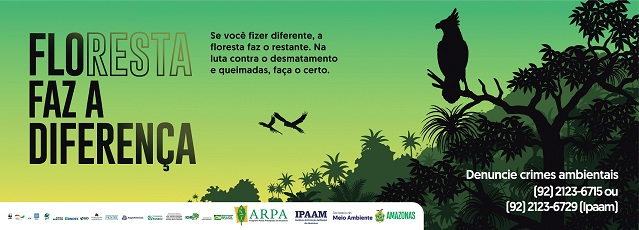
\includegraphics[width=5.90551in,height=2.125in]{./imgSAEB_7_POR/media/image16.png}

Disponível em :
\textless{}\href{https://meioambiente.am.gov.br/campanha-floresta-faz-a-diferenca/}{\uline{https://meioambiente.am.gov.br/campanha-floresta-faz-a-diferenca/}}\textgreater{}

Acesso em 6 de Abril 2023

Acima, pode-se ver um cartaz de conscientização sobre o desmatamento da
Amazônia. O uso e repetição de determinadas palavras e imagens tem como
finalidade sensibilizar os leitores para o problema do desmatamento.
Sobre o jogo de palavras presente no cartaz assinale a alternativa
correta:

\begin{enumerate}
\def\labelenumi{\alph{enumi})}
\item
  As diferenças entre os tamanhos de fontes são os únicos elementos
  responsáveis pela persuasão.
\item
  O texto traz explicações sobre as consequências das queimadas e
  desmatamento
\item
  O uso das variações da palavra `diferença' e `diferente' que se
  articulam para convidar a uma mudança de atitude
\item
  As imagens são os recursos de maior função persuasiva
\end{enumerate}

SAEB: - Identificar o uso de recursos persuasivos em textos verbais e
não verbais.

Bncc: EF67LP07)Identificar o uso de recursos persuasivos em textos
argumentativos diversos (como a elaboração do título, escolhas lexicais,
construções metafóricas, a explicitação ou a ocultação de fontes de
informação) e perceber seus efeitos de sentido.

\begin{enumerate}
\def\labelenumi{\arabic{enumi}.}
\item
  Incorreta. A escolha de fontes, tamanhos e cores é um fator importante
  para a compreensão imediata da mensagem do texto, porém, não é o único
  recurso utilizado com essa finalidade.
\item
  Incorreta. Embora o texto faça alusão ao desmatamento e às queimadas,
  não se encontram explicações sobre os termos e suas consequências.
\item
  Correta. Os diversos recursos modais e o jogo de sentido no emprego
  das palavras destacadas são os principais recursos de persuasão,
  sensibilização e chamada para mudança de atitudes presente no cartaz.
\item
  Incorreta. Embora as imagens contribuam para a compreensão da
  mensagem, de forma isolada não contribuem para o sentido da mensagem.
\end{enumerate}

\num{2}

\textbf{Fumaça de queimadas do Amazonas chega a São Paulo; moradores
relatam ``cheiro forte''}

Segundo a Climatempo, a nuvem de fumaça foi gerada por incêndios em
parte do Amazonas, Acre e Mato Grosso

Moradores da cidade de São Paulo relataram sentir cheiro de fumaça na
manhã desta sexta-feira (9).

Na quinta (8), a Climatempo havia alertado para a nuvem gerada por
queimadas em parte do Amazonas, Acre e Mato Grosso, que espalhou sobre o
Brasil, e que chegaria também em grande parte do Centro-Oeste, no Paraná
e até em parte do estado de São Paulo.

A Companhia Ambiental do Estado de São Paulo (CETESB) disse que a
Divisão de Qualidade do Ar da agência está investigando as fumaças e
monitorando a qualidade do ar.

``{[}A divisão{]} está fazendo uma apuração detalhada dos dados das
estações de monitoramento da qualidade do ar distribuídas pela RMSP
Informaremos assim que tivermos um dado mais consolidado sobre a
ocorrência'', diz a nota.

Disponível em
\textless{}\href{https://www.cnnbrasil.com.br/nacional/fumaca-de-queimadas-do-amazonas-chega-a-sao-paulo-moradores-relatam-cheiro-forte/}{\uline{https://www.cnnbrasil.com.br/nacional/fumaca-de-queimadas-do-amazonas-chega-a-sao-paulo-moradores-relatam-cheiro-forte/}}\textgreater.
Acesso em 7 de abril de 2023.

Assinale a alternativa que contém a parte da notícia denominada linha
fina:

\begin{enumerate}
\def\labelenumi{\alph{enumi})}
\item
  Fumaça de queimadas do Amazonas chega a São Paulo; moradores relatam
  ``cheiro forte''
\item
  ``{[}A divisão{]} está fazendo uma apuração detalhada dos dados das
  estações de monitoramento da qualidade do ar distribuídas pela RMSP
  Informaremos assim que tivermos um dado mais consolidado sobre a
  ocorrência'', diz a nota.
\item
  Moradores da cidade de São Paulo relataram sentir cheiro de fumaça na
  manhã desta sexta-feira (9).
\item
  Segundo a Climatempo, a nuvem de fumaça foi gerada por incêndios em
  parte do Amazonas, Acre e Mato Grosso
\end{enumerate}

Saeb: Identificar elementos constitutivos de textos pertencentes ao
domínio

jornalístico/midiático

\begin{enumerate}
\def\labelenumi{\arabic{enumi}.}
\item
  Incorreta. O trecho corresponde ao título da notícia.
\item
  Incorreta. O trecho corresponde ao corpo da notícia.
\item
  Incorreta. O trecho compõe o lide da notícia.
\item
  Correta. A linha fina aparece como uma introdução ao assunto da
  notícia e se localiza entre o título e lide.
\end{enumerate}

\num{3}

Uma parceria entre a Universidade Federal do Rio de Janeiro e a
Universidade Federal do Estado do Rio de Janeiro (Unirio) vem estudando
o vírus-T linfotrópico humano do tipo 1, o HTLV-1, retrovírus da mesma
família do HIV, associado a casos de leucemia e doenças
neurodegenerativas. A pesquisa recebeu investimento da Organização
Pan-Americana de Saúde (Opas/OMS) junto com outros estudos
latino-americanos e caribenhos que investigam doenças negligenciadas.
Embora descrito, na década de 1980, como um vírus associado ao câncer, o
HTLV ainda é pouco estudado e bastante desconhecido do público em geral.

\href{https://conexao.ufrj.br/2023/04/pesquisa-investiga-virus-negligenciado-que-pode-levar-a-doencas-neurodegenerativas-e-leucemia/}{\uline{https://conexao.ufrj.br/2023/04/pesquisa-investiga-virus-negligenciado-que-pode-levar-a-doencas-neurodegenerativas-e-leucemia/}}.
Acesso em 20 de Abr de 2023

O texto acima é um texto do gênero de divulgação científica pois:

\begin{enumerate}
\def\labelenumi{\alph{enumi})}
\item
  traz informações técnicas e de difícil compreensão
\item
  é escrito de maneira formal e dirigido a cientistas e estudiosos
\item
  traz informações sobre fatos do cotidiano
\item
  traz informações científicas em linguagem clara e acessível ao público
  geral
\end{enumerate}

Identificar elementos constitutivos de gêneros de divulgação científica

\begin{enumerate}
\def\labelenumi{\arabic{enumi}.}
\item
  Incorreta. O texto não apresenta linguagem técnica
\item
  Incorreta. O texto não é destinado apenas a cientistas
\item
  Incorreta. O trecho não aborda fatos cotidianos
\item
  Correta. O texto faz uso de linguagem clara e acessível para divulgar
  estudos científicos para o público em geral
\end{enumerate}

\num{4}

Il.mº. Sra. Diretora da Escola Estadual Ulysses Guimarães

Mariana Amaral Santos, aluna regularmente matriculada no sétimo ano do
ensino fundamental desta escola, vem respeitosamente solicitar à V. Sa a
expedição dos documentos necessários à sua transferência para outro
estabelecimento de ensino.

Nestes termos, pede deferimento.

Curitiba, 24 de setembro de 2022.

Texto adaptado.

Os gêneros textuais reivindicatórios são textos que circulam no campo da
vida pública e possuem função social e estrutura específicas. O texto
acima é um modelo de Requerimento pois tem como objetivo:

\begin{enumerate}
\def\labelenumi{\arabic{enumi}.}
\item
  convencer o destinatário a realizar uma ação importante.
\item
  solicitar formalmente ao destinatário a realização de uma ação.
\item
  mudar o comportamento do destinatário a partir da realização de ações.
\item
  informar formalmente o destinatário acerca da solicitação de ações.
\end{enumerate}

Identificar formas de organização de textos normativos, legais e/ou
reivindicatórios.

Bncc (EF67LP17)Analisar, a partir do contexto de produção, a forma de
organização das cartas de solicitação e de reclamação (datação, forma de
início, apresentação contextualizada do pedido ou da reclamação, em
geral, acompanhada de explicações, argumentos e/ou relatos do problema,
fórmula de finalização mais ou menos cordata, dependendo do tipo de
carta e subscrição) e algumas das marcas linguísticas relacionadas à
argumentação, explicação ou relato de fatos, como forma de possibilitar
a escrita fundamentada de cartas como essas ou de postagens em canais
próprios de reclamações e solicitações em situações que envolvam
questões relativas à escola, à comunidade ou a algum dos seus membros.

\begin{enumerate}
\def\labelenumi{\arabic{enumi}.}
\item
  Incorreta. O texto não pretende convencer
\item
  Correta. O texto pretende solicitar uma transferência de instituição
\item
  Incorreta. Não há indicação de mudança de atitude
\item
  Incorreta. O objetivo não é informar e sim solicitar
\end{enumerate}

\num{5}

ATO I

Cena I

Veneza. Uma rua. Entram Antônio. Salarino e Salânio.

ANTÓNIO - Não sei, realmente, porque estou tão triste. Isso me enfara; e
a vós também, dissestes. Mas como começou essa tristeza, de que modo a
adquiri, como me veio, onde nasceu, de que matéria é feita, ainda estou
por saber. E de tal modo obtuso ela me deixa, que mui dificilmente me
conheço.

SALARINO - Vosso espírito voga em pleno oceano, onde vossos galeões de
altivas velas - como burgueses ricos e senhores das ondas, ou qual vista
aparatosa distendida no mar - olham por cima da multidão de humildes
traficantes que os saúdam, modestos, inclinando-se, quando perpassam com
tecidas asas.

Shakespeare, William. O Mercador de Venza. Disponível em
\href{http://www.dominiopublico.gov.br/download/texto/cv000094.pdf}{\uline{http://www.dominiopublico.gov.br/download/texto/cv000094.pdf}}.
Acesso em 20 de Abr. de 2023

O trecho acima apresenta certas características, como discurso direto,
indicações de falas de personagens e rubrica que são características do
gênero textual:

\begin{enumerate}
\def\labelenumi{\alph{enumi})}
\item
  Dramático. Gênero dos textos criados para serem encenados
\item
  Poesia. Gênero composto por versos e estrofes
\item
  Conto. Gênero escrito em linguagem simples e com poucos personagens
\item
  Romance. Gênero que comporta narrativa longas e com muitos personagens
\end{enumerate}

Analisar elementos constitutivos de textos pertencentes ao domínio

literário.

\begin{enumerate}
\def\labelenumi{\arabic{enumi}.}
\item
  Correta. O texto acima é um exemplo de texto teatral ou dramático
\item
  Incorreta. O trecho acima não é composto por versos e estrofes
\item
  Incorreta. O trecho acima não apresenta características de conto
\item
  O trecho acima não possui características de conto
\end{enumerate}

\num{6}

Rogério Ceni deixou o São Paulo. Este é só mais um capítulo na história
de um clube que caminha a passos largos rumo ao buraco. A verdade é uma
só e dói para o apaixonado torcedor admitir: aquele São Paulo que era
modelo de administração e que num intervalo de três anos ganhou
Paulista, Libertadores, Mundial de Clubes e o tricampeonato brasileiro
acabou. Virou apenas lembrança.

\href{https://ge.globo.com/futebol/times/sao-paulo/noticia/2023/04/20/opiniao-vaidade-e-soberba-de-dirigentes-afundam-o-sao-paulo-rumo-a-um-futuro-preocupante.ghtml}{\uline{https://ge.globo.com/futebol/times/sao-paulo/noticia/2023/04/20/opiniao-vaidade-e-soberba-de-dirigentes-afundam-o-sao-paulo-rumo-a-um-futuro-preocupante.ghtml}}.
Acesso em 20 de Abr de 2023

A Notícia acima apresenta muitas opiniões e poucos fatos. Há um fato
expresso no texto por:

\begin{enumerate}
\def\labelenumi{\alph{enumi})}
\item
  Este é só mais um capítulo na história de um clube
\item
  A verdade é uma só e dói para o apaixonado torcedor
\item
  um clube que caminha a passos largos rumo ao buraco
\item
  O São Paulo num intervalo de três anos ganhou Paulista, Libertadores
  (...)
\end{enumerate}

Saeb: Distinguir fatos de opiniões em textos

\begin{enumerate}
\def\labelenumi{\arabic{enumi}.}
\item
  Incorreta. Este trecho representa a opinião do jornalista
\item
  Incorreta. Este trecho representa a opinião do jornalista
\item
  Incorreta. Este trecho representa a opinião do jornalista
\item
  Correta. Este trecho apresenta um fato
\end{enumerate}

\num{7}


\includegraphics[width=4.16667in,height=1.57292in]{./imgSAEB_7_POR/media/image17.png}

\href{http://www.arionaurocartuns.com.br/search?q=moradia}{\uline{http://www.arionaurocartuns.com.br/search?q=moradia}}.
Acesso em 20 de Abr de 2023.

A charge utiliza de recursos verbais e não verbais para provocar:

\begin{enumerate}
\def\labelenumi{\alph{enumi})}
\item
  Humor e reflexão
\item
  Crítica e tristeza
\item
  Humor e revolta
\item
  Crítica e alegria
\end{enumerate}

Saeb: Inferir, em textos multissemióticos, efeitos de humor, ironia e/ou
crítica.

Bncc: EF69LP03 Inferir e justificar, em textos multissemióticos --
tirinhas, charges, memes, gifs etc. --, o efeito de humor, ironia e/ou
crítica pelo uso ambíguo de palavras, expressões ou imagens ambíguas, de
clichês, de recursos iconográficos, de pontuação etc.

a)Correta. As charges em geral pretendem provocar humor e reflexão por
meio da crítica social

\begin{enumerate}
\def\labelenumi{\arabic{enumi}.}
\item
  Incorreta. Não pretende provocar tristeza, apesar de trazer temas
  difíceis
\item
  Incorreta. A charge não pretende causar revolta, embora provoque
  reflexão e crítica
\item
  Incorreta. A charge não pretende trazer mensagem de alegria
\end{enumerate}

\num{8}

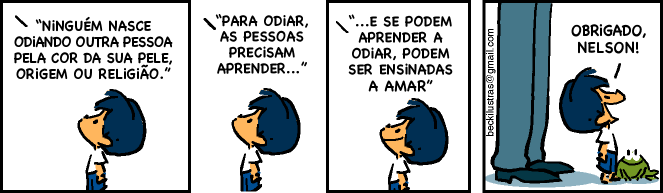
\includegraphics[width=5.90551in,height=1.72222in]{./imgSAEB_7_POR/media/image18.png}

\href{https://tirasarmandinho.tumblr.com/search/amor}{\uline{https://tirasarmandinho.tumblr.com/search/amor}}.
Acesso em 21 de Abr.

A tirinha acima faz referência a uma frase de Nelson Mandela. Sempre que
um texto faz referência a outro ou o toma como modelo de partida
utiliza-se o recurso chamado:

\begin{enumerate}
\def\labelenumi{\alph{enumi})}
\item
  Persuasão
\item
  Coesão
\item
  Metáfora
\item
  Intertextualidade
\end{enumerate}

Saeb: Analisar a intertextualidade entre textos literários ou entre
estes e outros

textos verbais ou não verbais.

Bncc: (EF67LP27) Analisar, entre os textos literários e entre estes e
outras manifestações artísticas (como cinema, teatro, música, artes
visuais e midiáticas), referências explícitas ou implícitas a outros
textos, quanto aos temas, personagens e recursos literários e semióticos

\begin{enumerate}
\def\labelenumi{\arabic{enumi}.}
\item
  Incorreta. Este não é um recurso de persuasão
\item
  Incorreta. Este não é um recurso de coesão
\item
  Incorreta. Neste exemplo não ocorre o uso de metáfora
\item
  Correta. O uso de outros textos como modelo ou ponto de partida é
  chamado de intertextualidade.
\end{enumerate}

\num{9}

Leia o trecho a seguir:

``O Rio Doce, que nós, Krenak, chamamos de Watu, nosso avô,é uma pessoa,
não um recurso, como dizem os economistas''

Krenak, Ailton. Ideias para adiar o fim do mundo.2ª Ed. São paulo:
Companhia da Letras, 2020, p.~40

O trecho acima traz importantes informações sobre:

\begin{enumerate}
\def\labelenumi{\alph{enumi})}
\item
  mitos e lendas que servem para ilustrar a cultura indígena
\item
  as diferenças entre a maneira de pensar os recursos naturais entre os
  indígenas e não indígenas
\item
  A língua falada pelos povos indígenas brasileiros no estado de Minas
  Gerais
\item
  uma história que é passada de geração em geração restrita aos povos
  indígenas brasileiros
\end{enumerate}

Saeb: Inferir a presença de valores sociais, culturais e humanos em
textos

literários.

Bncc:(EF69LP44) Inferir a presença de valores sociais, culturais e
humanos e de diferentes visões de mundo, em textos literários,
reconhecendo nesses textos formas de estabelecer múltiplos olhares sobre
as identidades, sociedades e culturas e considerando a autoria e o
contexto social e histórico de sua produção.

\begin{enumerate}
\def\labelenumi{\arabic{enumi}.}
\item
  Incorreta. O trecho não retrata um mito ou lenda
\item
  Correta. No trecho Ailton Krenak explica a maneira como os povos
  indígenas enxergam os recursos naturais
\item
  Incorreta. Apesar de trazer o termo utilizado para designar o rio, não
  traz informações sobre a língua
\item
  Incorreta. O trecho não faz referência à forma como essas questões são
  tratadas dentro da tradição indígena.
\end{enumerate}

\num{10}

Faxina correta da casa evita crise alérgica e possíveis problemas
respiratórios

Pessoas alérgicas devem evitar acúmulo de objetos dentro de casa,
principalmente no quarto.

Alérgica desde criança, a aposentada Glória Pordeus, 53 anos, viu os
problemas respiratórios serem agravados após se tornar portadora de
Lúpus, devido à baixa imunidade relacionada à doença. \textbf{Com isso,}
ela precisou redobrar os cuidados na hora de organizar a casa.
Especialistas alertam que pessoas alérgicas devem evitar acúmulo de
certos objetos, principalmente no quarto, e invés de usar vassoura para
limpar o chão, deve-se usar um pano úmido, e repassam dicas de como
manter o domicílio limpo sem comprometer a saúde.

\href{https://jornaldaparaiba.com.br/bichos/faxina-correta-da-casa-evita-crise-alergica-e-possiveis-problemas-respiratorios/}{\uline{https://jornaldaparaiba.com.br/bichos/faxina-correta-da-casa-evita-crise-alergica-e-possiveis-problemas-respiratorios/}}\textbf{.}

No texto acima, a expressão destacada se refere a:

\begin{enumerate}
\def\labelenumi{\alph{enumi})}
\item
  Limpeza redobrada do ambiente
\item
  Condição de saúde que faz com que os cuidados tenham que ser
  redobrados
\item
  Orientação médica sobre os cuidados com as crianças
\item
  Idade da paciente que precisa se cuidar cada vez mais
\end{enumerate}

Analisar os mecanismos que contribuem para a progressão textual.

\begin{enumerate}
\def\labelenumi{\arabic{enumi}.}
\item
  Incorreta.Esta informação aparece depois do recurso
\item
  Correta. O termo refere-se às doenças que exigem mais cuidados na hora
  da limpeza
\end{enumerate}

c)Incorreta. O termo não se refere a orientações médicas, e sim ao que
leva a precisar de certos cuidados

\begin{enumerate}
\def\labelenumi{\arabic{enumi}.}
\tightlist
\item
  Incorreta. Apesar de trazer a informação sobre a idade o termo não se
  refere a isso e sim à condição de saúde
\end{enumerate}

\num{11}

Veja o título da notícia em negrito e responda

\hypertarget{sedentuxe1rios-e-grudados-a-uma-tela.-o-que-mostra-o-maior-estudo-mundial-sobre-atividade-fuxedsica-de-jovens}{%
\section{\texorpdfstring{\textbf{Sedentários e grudados a uma tela. O
que mostra o maior estudo mundial sobre atividade física de
jovens}}{Sedentários e grudados a uma tela. O que mostra o maior estudo mundial sobre atividade física de jovens}}\label{sedentuxe1rios-e-grudados-a-uma-tela.-o-que-mostra-o-maior-estudo-mundial-sobre-atividade-fuxedsica-de-jovens}}

\hypertarget{segundo-os-dados-divulgados-nesta-sexta-feira-80-dos-adolescentes-do-mundo-nuxe3o-fazem-o-muxednimo-de-exercuxedcio-recomendado.-para-as-meninas-os-nuxfameros-suxe3o-ainda-piores}{%
\section{Segundo os dados divulgados nesta sexta-feira, 80\% dos
adolescentes do mundo não fazem o mínimo de exercício recomendado. Para
as meninas, os números são ainda
piores}\label{segundo-os-dados-divulgados-nesta-sexta-feira-80-dos-adolescentes-do-mundo-nuxe3o-fazem-o-muxednimo-de-exercuxedcio-recomendado.-para-as-meninas-os-nuxfameros-suxe3o-ainda-piores}}

\href{https://brasil.elpais.com/brasil/2019/11/18/actualidad/1574086350_697117.html}{\uline{https://brasil.elpais.com/brasil/2019/11/18/actualidad/1574086350\_697117.html}}.
Acesso em 20 de Abr de 2023

A frase que apresenta uma hipérbole é:

\begin{enumerate}
\def\labelenumi{\alph{enumi})}
\item
  Sedentários e grudados a uma tela
\item
  O queria o maior estudo mundial
\item
  adolescentes do mundo não fazem o mínimo
\item
  Para as meninas os números são ainda piores
\end{enumerate}

Saeb:Analisar o uso de figuras de linguagem como estratégia
argumentativa

\begin{enumerate}
\def\labelenumi{\arabic{enumi}.}
\item
  Correta. O termo grudados a uma tela representa figura de linguagem
\item
  Incorreta. O termo não apresenta figura de linguagem
\item
  Incorreta. O termo não apresenta figura de linguagem
\item
  Incorreta. O termo não apresenta figura de linguagem
\end{enumerate}

\num{12}

Os especialistas consultados consideram que o mais previsível durante as
próximas semanas é ``um crescimento substancial das detecções da
ômicron, que já começa a ser percebido, até que a nova variante
substitua a delta, \textbf{algo que poderia ocorrer} em cerca de três
semanas'', explica Federico García, chefe de Microbiologia do Hospital
San Cecilio (Granada), um centro de referência para a Andaluzia
oriental.

\href{https://brasil.elpais.com/internacional/2021-12-13/agencia-de-saude-publica-da-ue-avisa-que-a-omicron-se-propaga-pelo-continente-mais-rapido-do-que-e-detectada.html}{\uline{https://brasil.elpais.com/internacional/2021-12-13/agencia-de-saude-publica-da-ue-avisa-que-a-omicron-se-propaga-pelo-continente-mais-rapido-do-que-e-detectada.html}}.
Acesso em 21 de Abr de 2023

A expressão em destaque é um conectivo de coesão textual. A palavra algo
no texto se refere a:

\begin{enumerate}
\def\labelenumi{\alph{enumi})}
\item
  acontecimentos inesperados
\item
  crescimento das detecções
\item
  substituição da variante ômicron pela delta
\item
  mortes por covid
\end{enumerate}

Saeb:Analisar os processos de referenciação lexical e pronominal.

\begin{enumerate}
\def\labelenumi{\arabic{enumi}.}
\item
  Incorreta. O conectivo não se refere a acontecimentos inesperados
\item
  Incorreta. Embora esteja na mesma frase, algo não se refere a este
  fato
\item
  Correta. O cientista afirma que a substituição deve ocorrer em cerca
  de três semanas
\item
  Incorreta. O texto não traz informações sobre mortes por covid
\end{enumerate}

\num{13}

\textbf{A prática da leitura é o grande desafio da escola e das famílias
para os alunos e filhos. É comum encontrarmos aqueles que não gostam de
ler --} mas isso só até descobrirem o prazer dessa atividade. Se as
crianças fossem estimuladas no lado prazeroso da leitura, teríamos mais
leitores e não apenas compradores de livros. \textbf{A literatura é um
dos principais meios de transmissão cultural e,} como nos mantém em
contato com a imaginação, estimula a nossa criatividade.

https://g1.globo.com/Noticias/Vestibular/0,,MUL723077-5604,00-OPINIAO+COMO+FAZER+DE+SEU+FILHO+UM+LEITOR.html

Os trechos em destaque apresentam argumentação do tipo

\begin{enumerate}
\def\labelenumi{\alph{enumi})}
\item
  Argumento de autoridade
\item
  Argumento de exemplo
\item
  Argumento de consenso
\item
  Argumento por ilustração
\end{enumerate}

Avaliar a eficácia das estratégias argumentativas em textos de
diferentes gêneros.

\begin{enumerate}
\def\labelenumi{\arabic{enumi}.}
\item
  Incorreta. O trecho não cita quem profere as afirmações, portanto não
  se sabe se é um argumento de autoridade
\item
  Incorreta. O trecho não traz exemplos
\item
  Correta. O trecho utiliza de argumentos que, em geral, não geram
  discordância
\item
  Incorreta. Neste caso, não são citados exemplos como estratégia de
  argumentação
\end{enumerate}

\num{14}

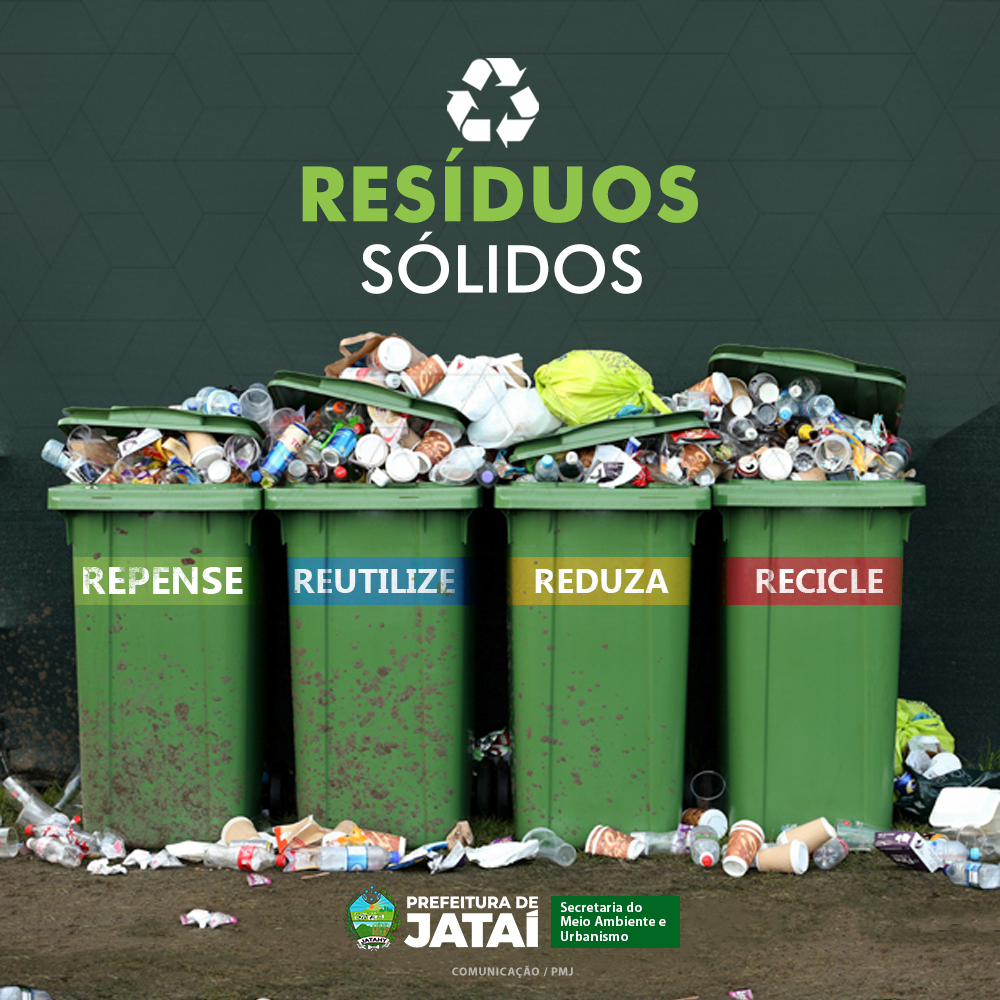
\includegraphics[width=5.90551in,height=5.90278in]{./imgSAEB_7_POR/media/image19.png}

\href{https://www.jatai.go.gov.br/separe-seu-lixo-de-forma-adequada/}{\uline{https://www.jatai.go.gov.br/separe-seu-lixo-de-forma-adequada/}}.Acesso
em 22 de Abr de 2023

Na imagem acima, pode-se perceber diversos recursos para que a mensagem
seja transmitida de maneira eficiente e imediata. No caso da escolha dos
verbos utilizados é correto afirmar que:

\begin{enumerate}
\def\labelenumi{\alph{enumi})}
\item
  Os verbos no imperativo afirmativo sugerem uma ação
\item
  O uso dos verbos no infinitivo indica uma instrução
\item
  Os verbos no subjuntivo indicam uma advertência
\item
  O uso dos verbos no infinitivo indica uma ordem
\end{enumerate}

Analisar os efeitos de sentido dos tempos, modos e/ou vozes verbais com
base no gênero textual e na intenção comunicativa.

\begin{enumerate}
\def\labelenumi{\arabic{enumi}.}
\item
  Correta. O verbo no modo imperativo tem a função de instrução e neste
  caso, de maneira afirmativa, sugere uma mudança de atitude por parte
  do leitor
\item
  Incorreta.Os verbos não estão no infinitivo
\item
  Incorreta. Os verbos não estão no modo subjuntivo e não indicam
  advertência
\item
  Incorreta. O uso de verbos no imperativo, como no exemplo podem
  indicar uma ordem, porém a imagem não traz verbos no infinitivo
\end{enumerate}

\num{15}


\includegraphics[width=5.90551in,height=3.15278in]{./imgSAEB_7_POR/media/image20.png}

\href{https://www.tre-sp.jus.br/comunicacao/noticias/2022/Marco/tuitaco-roledaseleicoes-alcanca-trending-topics-no-twitter}{\uline{https://www.tre-sp.jus.br/comunicacao/noticias/2022/Marco/tuitaco-roledaseleicoes-alcanca-trending-topics-no-twitter}}.
Acesso em 20 de Abr de 2023

Analisando a campanha acima, destinada ao público jovem, é correto
afirmar que:

\begin{enumerate}
\def\labelenumi{\alph{enumi})}
\item
  a campanha utiliza linguagem formal para atingir o público alvo
\item
  a campanha utiliza linguagem informal para atingir todos os públicos
\item
  a campanha utiliza linguagem informal para atingir o público alvo
\item
  a campanha utiliza linguagem formal para atingir todos os públicos
\end{enumerate}

Avaliar a adequação das variedades linguísticas em contextos de uso.

\begin{enumerate}
\def\labelenumi{\arabic{enumi}.}
\item
  Incorreta. A campanha não utiliza linguagem formal
\item
  Incorreta. Apesar de fazer uso da linguagem informal a campanha tem um
  público alvo bem claro
\item
  Correta. A campanha faz uso de linguagem informal para atingir os
  jovens
\item
  Incorreta. A campanha não faz uso de linguagem formal, nem pretende
  atingir todos os públicos
\end{enumerate}
